%!TEX TS-program = xelatex 
%!TEX encoding = UTF-8 Unicode

% Modify the following line to match your school
% Available options include `Harvard`, `Princeton`, and `NYU`.
\documentclass[
    School=Harvard,
    % margin=1in,
    twoside,
    openright,
    BCOR10mm,
]{Dissertate}% only use twoside and openright when printing!

\newcommand\FanoPlane[1][1cm]{%
\begin{tikzpicture}[
mydot/.style={
  draw,
  circle,
  fill=black,
  inner sep=1.5pt}
]
\draw[thick]
  (0,0) coordinate (A) --
  (#1,0) coordinate (B) --
  ($ (A)!.5!(B) ! {sin(60)*2} ! 90:(B) $) coordinate (C) -- cycle;
\coordinate (O) at
  (barycentric cs:A=1,B=1,C=1);
\draw[thick,red] (O) circle [radius=#1*1.717/6];
\draw[thick,printBlue] (C) -- ($ (A)!.5!(B) $) coordinate (LC); 
\draw[thick,violet] (A) -- ($ (B)!.5!(C) $) coordinate (LA); 
\draw[thick,SchoolColor] (B) -- ($ (C)!.5!(A) $) coordinate (LB); 
% \foreach \Nodo in {A,B,C,O,LC,LA,LB}
%   \node[mydot] at (\Nodo) {};    
  \node[circle,inner sep=0.4pt,draw=black,fill=white,minimum size=0.15cm](smallRect) at (A) {C};
  \node[circle,inner sep=0.4pt,draw=black,fill=white,minimum size=0.15cm](smallRect) at (B) {E};
  \node[circle,inner sep=0.4pt,draw=black,fill=white,minimum size=0.15cm](smallRect) at (C) {A};
  \node[circle,inner sep=0.4pt,draw=black,fill=white,minimum size=0.15cm](smallRect) at (O) {D};
  \node[circle,inner sep=0.4pt,draw=black,fill=white,minimum size=0.15cm](smallRect) at (LC) {G};
  \node[circle,inner sep=0.4pt,draw=black,fill=white,minimum size=0.15cm](smallRect) at (LA) {F};
  \node[circle,inner sep=0.4pt,draw=black,fill=white,minimum size=0.15cm](smallRect) at (LB) {B};
\end{tikzpicture}%
}

\begin{document}
\newfontfamily\hindifont{Noto Sans Devanagari}[Script=Devanagari]
% the front matter
% Some details about the dissertation.
\title{Rational Thaumaturgy \\ \vspace{0.35cm} \Large Formal Variegation and the Formalization of Event Groups in the Music of Jean Barraqué, Francisco Guerrero Marín, Trevor Bača, and Gregory Rowland Evans}
\author{Gregory Rowland Evans}
\advisor{David Gompper}

% ... about the degree.
\degree{Doctor of Philosophy}
\field{Music Composition}
\degreeyear{2024}
\degreemonth{May}
\department{Music}

% ... about the candidate's previous degrees.
\pdOneName{B.M.}
\pdOneSchool{University of Cincinnati}
\pdOneYear{2017}

\pdTwoName{M.M.}
\pdTwoSchool{University of Miami}
\pdTwoYear{2019}
\maketitle
\copyrightpage
\justifying
\dedicationpage
\frontispiece
\acknowledgments
\title{Rational Thaumaturgy: Formal Variegation and the Formalization of Event Groups in the Music of Jean Barraqué, Francisco Guerrero Marín, Trevor Bača, and Gregory Rowland Evans} % redefine title for prettier abstract page
\scholarlyabstractpage
\publicabstractpage
\tableofcontents
%\authorlist
\cleardoublepage
\phantomsection
\addcontentsline{toc}{chapter}{List of Tables}
\listoftables
\cleardoublepage
\phantomsection
\addcontentsline{toc}{chapter}{List of Figures}
\listoffigures
% list of symbols?
\cleardoublepage
\phantomsection
\addcontentsline{toc}{chapter}{Listings}
\lstlistoflistings
%*******************************************************
% Symbols
%*******************************************************
%\phantomsection
\pdfbookmark[1]{List of Symbols}{symbols}
\markboth{\uppercase{List of Symbols}}{\uppercase{List of Symbols}}
\chapter*{List of Symbols}
\addcontentsline{toc}{chapter}{List of Symbols}
\begin{tabular}{cp{0.6\textwidth}}
    $!$ & factorial \\
    $\subset$ & is a proper subset of \\
    $\in$ & is member of \\
    $\not\subset$ & is not a proper subset of \\
    $\%$ & modulo, or remainder \\
    ϕ & phi, or $\frac{1 + \sqrt{5}}{2}\approx$ 1.61803...\\
    π & pi, or $\frac{circumference}{diameter}\approx$ 3.14159... \\
    $\cap$ & set intersection \\
    $\cup$ & set union \\
    $\Sigma$ & sum \\
\end{tabular}\\

%*******************************************************

%*******************************************************
% Acronyms
%*******************************************************
%\phantomsection
\pdfbookmark[1]{Acronyms}{acronyms}
\markboth{\uppercase{Acronyms}}{\uppercase{Acronyms}}
\chapter*{Acronyms}
\addcontentsline{toc}{chapter}{Acronyms}
\begin{acronym}[UMLX]
    \acro{ANG}{automatic notation generator}
    \acro{API}{application programming interface}
    \acro{CLT}{col legno tratto}
    \acro{CSD}{composition as software development}
    \acro{FSC}{formalized score control}
    \acro{GUI}{graphic user interface}
    \acro{LIFO}{last in first out}
    \acro{LILO}{last in last out}
    \acro{MIDI}{musical instrument digital interface}
    \acro{OB}{on the bridge}
    \acro{PDF}{portable document format}
    \acro{SB}{slow bow}
    \acro{SP}{sul ponticello}
    \acro{ST}{sul tasto}
    \acro{XFB}{extremely fast bow}
    \acro{XSB}{extremely slow bow}
    \acro{XSP}{extremely sul ponticello}
    \acro{XST}{extremely sul tasto}
\end{acronym}
%*******************************************************

\doublespacing

% \cleardoublepage % doesn't work ...
% include each chapter...
\setcounter{chapter}{-1}  % start chapter numbering at 0
% \justifying
%%% EXPERIMENTAL HEADERS
% \usepackage{fancyhdr}
\pagestyle{fancy}
% \fancyhf{} % clear all header and footer fields
\fancyhead[CE]{R~A~T~I~O~N~A~L~~~~T~H~A~U~M~A~T~U~R~G~Y} 
\fancyhead[CO]{CHAPTER \thechapter: \leftmark}
% \fancyfoot[LE,RO]{\thepage}
\renewcommand{\chaptermark}[1]{\markboth{\MakeUppercase{#1}}{}}
\renewcommand{\headrulewidth}{0.4pt}
% \renewcommand{\footrulewidth}{0.4pt}
%%%%
\begin{savequote}[75mm]
It is the organization of a piece which helps the listener to keep the idea in mind, to follow its development, its growth, its elaboration, its fate.
\qauthor{Arnold Schönberg\footnote{\citet[381]{schonberg}}}
\end{savequote}

\chapter{Introduction}
\pagenumbering{arabic}
\label{introduction}

% \lettrine[lines=2,slope=-2pt,nindent=2pt]{\textcolor{SchoolColor}{O}}{n March 11, 2020}

\lettrine[lines=3]{\setmainfont{GoudyInitialen}[Path=./fonts/, Extension = .ttf]\color{printGreen}O}{n March 11, 2020} my first string quartet Hamonshū\index{Evans, Gregory Rowland!compositions!\textit{Hamonshū}} was premiered by the JACK quartet\index{JACK Quartet} alongside the works of several of my classmates in the composition department at the University of Iowa. While I was incredibly proud of the entire concert, I felt a slight uneasiness at the similarity between all of the works. When requesting feedback from some of my mentors and colleagues, one criticism stood out: the criticism that the piece did not have a clear formal arc. The work consists of seven relatively static panels of texture. As I listened back to each of the pieces on the concert, I found that this was what I had perceived as the connecting thread of similarity. The works were not activating my sense of memory through their formal architecture.\marginpar{Nevertheless, I was deeply inspired by the beauty of these works and I have been lucky to be able to interact with such talented colleagues.}

%\marginpar{The formatting of the margin paragraph definitely leaves something to be desired. It is good for informal, brief asides.}

\section{Origins}

In the course of my composition studies during both of my previous degrees, I summarized my growth in one primary technique. As an Undergraduate I spent most of my time learning how to create interesting musical materials, not just through harmonic and rhythmic innovation, but also by having a deep connection to the physical properties of the instrumental apparatus and even electronic manipulation of sound. As a Master's student, I developed a strong framework for compositional formalization in the Python\footnote{\url{https://www.python.org/}} programming language through the use of the Abjad\footnote{\url{https://abjad.github.io/}} \ac{API} for \ac{FSC}. This allowed me to develop rigorous systems for material generation which could be directly exported as Lilypond\footnote{\url{https://lilypond.org/}} files, cutting down the timeline required to compose formalized music.\marginpar{Obviously I learned more than one thing from each of my mentors.} After the premiere of Hamonshū\index{Evans, Gregory Rowland!compositions!\textit{Hamonshū}} I decided that the main field of compositional inquiry I needed to pursue during my Doctoral studies would be understanding the nature of the dramatic arc of large-scale formal systems. I was specifically searching for a way to approach the manipulation of aspects of form which could be integrated into my understanding of musical modernism.

I have never felt that I have understood the expressive role of the composer in modernity and as a result, I have been looking for systems which allow me to feel like I am in control of my music. Certainly, aspects of creative practice are perplexing or mysterious, even to the artist, but I found myself genuinely dumbfounded as to what I was doing when I sat down at my desk to compose. Gradually, I developed perspectives on rhythm, harmony, orchestration, and performing techniques, all within a highly rational framework. However, the question of how to deal with large-scale formal changes eluded me. In fact, I was resistant to the idea of allowing any ``changes'' in the flow of my music at all. This would mean that some elements of the work would not be developmentally related to one another. I eventually abandoned this need for total material inter-connectivity due to my experience with the music of two specific composers. In this dissertation, after a brief discussion of a negative example: Jean Barraqué's \textit{Sonate pour piano},\index{Barraqué, Jean!compositions!\textit{Sonate pour piano}} I will analyze two works which have had a significant impact on the way I think of composing large-scale forms: \textit{Rhea} by Francsico Guerrero\index{Guerrero Marín, Francisco!compositions!\textit{Rhea}} and \textit{Akasha}\index{Baca, Trevor!compositions!\textit{Akasha}} by Trevor Bača. In the works, the rational ordering of events of distinct genetic origin provide a formalist approach to large-scale form rather than the static uniformity of much early modernist music. These works suggest to me that the use of multiple generative processes within a work is not contradictory to the project of formalization. These pieces first interested me because I felt I could hear their structures. They gave me a psychological sensation of \textit{feeling} the form come into being in both the \textit{pro}gnostic and \textit{retro}gnostic fields of my memory while still engaging with the language of musical modernism. After the analytic chapters, I will summarize the shared characteristics of two of my own works, \textit{Polillas}\index{Evans, Gregory Rowland!compositions!\textit{Polillas}} for string quartet and \textit{Alu} for sinfonietta.\index{Evans, Gregory Rowland!compositions!\textit{Alu}}

\section{Modernism}

I decided to study form in contemporary music because of certain compositional trends which I noticed in contemporary music associated with the avant-garde. The Schönbergian approach to atonal pitch construction, specifically the twelve-tone system, is deliberately oriented toward a disintegration of tonal hierarchy,\footnote{\citet[207]{schonberg}} replacing tonal syntax with a new structuring principle which can often produce a sense of undifferentiated, saturated harmonic space.\footnote{\citet[39]{stockhausen}} This challenges the composer to organize musical discourse in ways other than through tonal pitch-centricity. When learning to analyze form in tonal music, it is the cadence which most clearly signifies the boundaries between themes,\footnote{\citet[34]{white}} but without cadences these sections could be better identified by their motivic content — in William Drabkin's article ``Theme'' in Grove Music Online, he makes the comment that the 12-tone series of a composition could \textit{itself} be considered the theme of a work and all statements of the series are developments or variations of that theme.\footnote{\citet{grove}} Likewise, the audience is also forced to listen for different orienting qualities.\index{Baca, Trevor}
\index{Barraqué, Jean}
\index{Boulez, Pierre}
\index{Evans, Gregory Rowland}
\index{Ferneyhough, Brian}
\index{Guerrero Marín, Francisco}

In the era of pointillistic music, reaching its culmination during the 1950's, the same kinds of approaches used to liberate harmony from cultural referentiality were applied to other sonic dimensions, for instance serializing rhythmic durations to disintegrate expressionist gestural vocables.\footnote{\citet[22]{ferneyhough}} After the surge of point-music, several modernist composers seemed to be looking for alternatives to compositional methods which proliferate musical ideas from a single motivic kernel.\footnote{\citet[81]{griffiths}} Stockhausen developed his theory of groups, Xenakis developed statistical composition, and some composers developed, after Stravinsky, what Jonathan Cross calls \textit{block forms}.\footnote{\citet[20]{cross}} These developments encouraged me that modernist thinking does not, by necessity, produce music with the æsthetic of sameness, rather contrast and differentiation can be controlled with the same level of precision as other facets of the musical surface.

\subsection{Is there a good definition of modernism?}

It is difficult to precisely define musical modernism\footnote{\citet[15]{legacy}} or even modernism as a whole.\footnote{\citet[2]{oxford-modernisms}} Recent developments in the study of modernism reveal a picture of an artistic movement of many, sometimes contradictory, ideas. \textit{The Oxford Handbook of Modernisms} describes many diverse strands of modernism, not only musical modernism, which promote queer and feminist readings, ``challeng[ing] [...] earlier accounts of modernism as a pre-eminently masculine enterprise.''\footnote{\citet[1]{oxford-modernisms}} Andrew Timms, in his chapter in \textit{The Modernist Legacy: Essays on New Music}, argues that the nature of musical modernism is far more multifaceted than can be expressed in a simple catalogue of ideologies. However, he concedes that modernism, broadly, encompasses interests in Formalism, Positivism, and Rationality. Formalism is defined as the tendency to define a strict series of axioms which are applied to the production of a given work. José L. Besada suggests that formalism can be seen as an inversion of modeling.\footnote{\citet[50]{besada}} Modeling applies the rules of an existing system to new goals, while formalization is ``the quest of the relevant syntax and axioms that may consolidate the logic of an intuited model.''\footnote{\citet[50]{besada}} Jonathan Cross suggests that musical modernism is not a monolithic ideological formation by analyzing the influence of certain aspects of the music of Igor Stravinsky on subsequent generations of composers.\footnote{\citet[4]{cross}}

A significant quality of Stravinsky's music which Cross links to an anti-organicist modernism is the \textit{drobnost}, or \textit{splinteredness}, of his works: ``the quality of being formally disunified, a sum-of-parts.''\footnote{\citet[10]{cross}} This fits well into other modernist ideals of fragmentation. Cross identifies Stravinsky's blocks as non-developmental or non-teleological,\footnote{\citet[10]{cross}} however my analysis of Trevor Bača's \textit{Akasha} in chapter \vref{Chapter2} shows the potential for developmental directionality in sectional form.

Discreet generative methodologies coexisting within a single work need not disqualify that work from inheriting critical modernist meanings. The psychological affect of different compositional strategies can be brought to bear within a single work. The hierarchical framework of tonal structure or rhythmic-motivic development can be replaced with a narrative framework which recognizes, even emphasizes, memory as an active component of the listening experience. The narrative of recurrent (versus episodic) materials, local and long-term development strategies, and identifiably distinct moments of different psychological time-weight are, for me, more than enough to engender an enlivened attentiveness to listening. In the introduction to \textit{The Modernist Legacy}, Björn Heile advocates for the term ``critical modernism'' to refer to a more expansive view of current modernist practices and quotes Peter Bürger saying:

\begin{quote}
    \singlespacing
    ``Instead of propagating a break with modernism under the banner of the postmodern, I count on its dialectical continuity. That means that æsthetic modernism must also recognize as its own much that it has until now rejected. This is, no more tabooing of tonality, representation, and traditional literary forms; but at the same time distrust of this material and of the appearance of substantiality which emanates from it. The recourse to past stocks of material must be recognized as a modern procedure, but also an extremely precarious one...''\footnote{\citet[5-6]{legacy}}
\end{quote}

\subsection{The Magical Metaphor}

Lois Fitch calls Brian Ferneyhough a post-modern modernist due to his rejection of grand narratives and the softness and changeability of his formalism.\footnote{\citet[159]{legacy}} During the course of a piece, Ferneyhough will often change procedures or even intervene upon the resultant material in order to achieve his desired results.\footnote{\citet[96]{toop}} This terminology can probably also be applied to the compositional behaviors of both Bača and myself. Instead, Bača reaches for a relationship to magical realism in his program notes for his work \textit{(HARMONY)}. Key to the magical metaphor is the concept of enciphering. The creation of talismans or the casting of spells was often associated with the inscription of a magical text. Encoding systems, while having every-day, functional use, can begin to be forgotten over time, confounding future generations who see enciphered text as holding a secret, perhaps a secret of magical significance. Some examples of encoding systems are the Hebrew Gematria or cipher runes on rune stones such as the Rökstenen, whereby a hidden meaning may be covered over by another, or hidden entirely.\footnote{Kennings, while less technical, also represent a kind of cipher.}\marginpar{The Rotas-Sator square has appeared in various orientations. The table here is a reproduction of a square engraved in a wall in Oppède-le-Vieux, France. While the meaning of the text is not precisely clear, the square has been used as a magical talisman to extinguish fire, heal wounds, and cure disease. There is no single, historical use of the square in magic practices.} Bača's composition software \textit{Abjad} is named after such a system: the abjad numerals. There is also a convenient history of magical thinking's influence over musical modernism as illustrated by Webern's use of the Rotas-Sator square for inspiration of his work \textit{Concerto for Nine Instruments} op.24:\footnote{\citet[5]{webern-sator}}

\begin{table}[H]
\centering
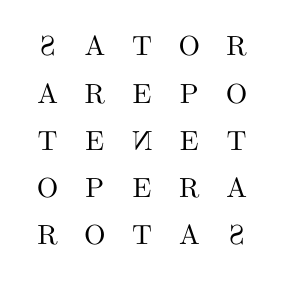
\begin{tikzpicture}[scale=0.6] % Adjust the scale factor as needed
    % Draw the Sator Square
    % \draw (0,0) grid (5,5);
    
    % Words in the Sator Square
    \node at (0.5,4.5) {\reflectbox{S}};
    \node at (1.5,4.5) {A};
    \node at (2.5,4.5) {T};
    \node at (3.5,4.5) {O};
    \node at (4.5,4.5) {R};
    
    \node at (0.5,3.5) {A};
    \node at (1.5,3.5) {R};
    \node at (2.5,3.5) {E};
    \node at (3.5,3.5) {P};
    \node at (4.5,3.5) {O};
    
    \node at (0.5,2.5) {T};
    \node at (1.5,2.5) {E};
    \node at (2.5,2.5) {\reflectbox{N}};
    \node at (3.5,2.5) {E};
    \node at (4.5,2.5) {T};
    
    \node at (0.5,1.5) {O};
    \node at (1.5,1.5) {P};
    \node at (2.5,1.5) {E};
    \node at (3.5,1.5) {R};
    \node at (4.5,1.5) {A};
    
    \node at (0.5,0.5) {R};
    \node at (1.5,0.5) {O};
    \node at (2.5,0.5) {T};
    \node at (3.5,0.5) {A};
    \node at (4.5,0.5) {\reflectbox{S}};
\end{tikzpicture}
\caption{Sator square}
    \label{tab:sator}
\end{table}

\textit{Thaumaturgy} is the art of ``wonder working.'' This can either be associated with Christian, saintly miracles or with other magical practices. In his \textit{Mathematicall Praeface to Elements of Geometrie of Euclid of Megara}, John Dee refers to thaumaturgy as the art of assembling mechanical objects of mathematical design. These machines were often attributed to magic by the uninitiated.\footnote{\citet{thaumaturgy}} Here we find an attractive metaphor: by the rational enciphering of a text or the mathematical assemblage of an object, onlookers may be astounded as if by the conjuring of magic. We can then refer to the æsthetic project of Trevor Bača's music as \textbf{Rational Thaumaturgy}\footnote{This term is borrowed from the novel \textit{Jonathan Strange \& Mr Norrell} by Susanna Clarke, a book which tells a fictionalized history of England and magical scholarship. While in the novel the term \emph{rational thaumaturgy} comes to represent the intellectual activities of non-practicing magicians (a class of individual often derided by the practicing magicians), no such negative connotation is intended here.}\marginpar{This terminology represents a slight rebranding of the title of Trevor Bača's dissertation: \emph{Magic Constructivism.}} in contrast to Francisco Guerrero's \textbf{Scientistic Romanticism}.\footnote{Scientistic romanticism refers to Guerrero's tendency to fetishize mathematics or scientific structures without having as deep an understanding of them as, say, Iannis Xenakis. In this way, Guerrero has a faith in the scientific aspects of the work giving meaning, truth, or beauty to his works. The stance is a modernist faith in progress in science as opposed to Bača's stance of encoded communication.} The artist's statement on Bača's website reads:

\begin{quote}
    \singlespacing
``I understand my music as emotive encoding. I write because I feel an emotional compulsion to write — to give form to fantastic or impossible colors and shapes as sound and as pleasure — and, yet, when I write, I am intensely aware of the fact that I am setting up and taking apart a code. I write for different combinations of instruments in chamber and orchestral settings and the written score is an important part of how I work. The act of score preparation is, for me, an emotional effort deeply concerned with the weight and energy and physical charge of raw and vibrant sounds, and, in equal measure, a type of work that is surpassingly symbolic, intimately bound up with the networks of potential meaning set up by marks on the page. I reject any dichotomy that pits the analytic against the emotional. Symbols can, and do, cut like knives. And I work for a music that is everywhere an emotional play of symbols, complete with all the almost unworkable contradictions such a play of symbols carries.

I don't understand either the societal or psychological parts of the composer role. And I would just as soon replace it with some other type of work carrying some other type of baggage. Sorcery, perhaps. A special appeal to concentration, with concern for a secret language of symbols, a secret way of reading the events and details of the natural world. I want music to be an intensely shared and public experience. And I want the intensity of that experience to result, at least in part, from an effort of decipherment, and translation, on all our parts.

My music comes back again and again to a constellation of images, and desire. The beauty of reflected and refracted light. The relationships between code and power and time. The assertion of power and importance in an everyday type of living. The delicacy of flowers and their parts. And networks of people and our relationships. I believe that there is something utterly human in rendering flashes of these ideas as symbols on the page, designed specifically for experience in some other, potentially unknown, place.''\footnote{\citet{bacawebsite}}
\end{quote}

By comparison, Ferneyhough describes his use of formalization in the following way:

\begin{quote}
    \singlespacing
    ``I think the use of any structure is [...] to enable one to have a framework within which one can meaningfully work at any given moment [...] it is a state of affairs at any given moment, and if you have worked the systems properly, then you have left yourself enough freedom to be able to react in a totally individual, and spontaneously significant fashion. Structures for me are not there to produce material; they're there to restrict the situation in which I have to compose.''\footnote{\citet[62]{toop}}
\end{quote}

From this perspective, formalization need not be used to \emph{justify} compositional decisions, rather it provides a situation which \emph{provokes} creative thinking. This is the aspect of modernist structuralism which I find the most exciting and the reason I specifically sought a loose but formalizeable approach to large-scale form.

\section{Rational Thaumaturgy}

While it certainly can be said that composers like Milton Babbitt, Francisco Guerrero, or Iannis Xenakis sought a scientistic justification for their artistic goals, the same cannot be said of composers such as Jean Barraqué, Pierre Boulez, Brian Ferneyhough, or Trevor Bača; whose use of systematic operations is disguised by a degree of composerly agency to modify the results of systematized products or through the implementation of ``cannibalizing'' systems which disguise themselves and cannot be reverse-engineered through analysis without recourse to sketch materials. The magical metaphor of \emph{Rational Thaumaturgy}, then, opens up an æsthetic category under the broader heading of modernism which encompasses works of this type which make use of modernist techniques and principles without the ethea of futurism or scientism which are often associated with such techniques.

\subsection{Analysis Beyond the Catalogue}

How should such a music be analyzed? What does an analysis intend to reveal? Analysis is an art-form in itself; sometimes revealing more about the orientations of the analyst than of anything substantive in the work itself. Should an analysis reveal the generative process of a work, consistencies within the behavior of a work or a group of works? What about the cultural context? All of these seem to be valuable avenues of exploration but perhaps analytic focus should be constrained to a specific category rather than aiming for unending comprehensiveness.

In the past I have struggled with understanding the nature and process of music analysis. What is music analysis and what is it for? In university we are often trained in a kind of rote analysis of labeling. However analysis is more than the mere identification of elements within a composition; the purpose of analysis is the understanding of musical style.\footnote{\citet[1]{white}} Pierre Boulez makes an interesting proposal for a different kind of analysis:

\begin{quote}
\singlespacing
``What is much more important in this case is the dialectic of composition [...] what may be called figured, or `ciphered,' analyses of this music are legion [...]. What is rewarding is to observe the dialectic of events, to obtain a bird's-eye view of the whole procedure and see how the composer contrives to formulate his thinking by means of such a system — that really does open up many more lines of inquiry.''\footnote{\citet[116]{boulez}}
\end{quote}

The nature of an analytic expression is primarily defined by the profession of the author. A musicologist might produce an analysis in order to say something about history or culture, a theorist might desire to communicate something about the mathematical properties latent in a musical schema, or a composer might wish to reveal properties of compositional craft which they find beautiful and therefore valuable. \marginpar{I think I have only been able to learn the craft of composition through the analysis of music and subsequent assimilation or rejection of the revealed properties of a work.} Boulez suggests that the indentification and labeling of materials and structures ought only to be done in service of understanding the transformation or interralatedness of structures across the whole of a composition:

\begin{quote}
\singlespacing
``Far the most important thing is to observe the existence of points shared 
 by different structures, and to mark the different areas of a work composed of such-and-such characteristics; to see how, in one section, certain features are avoided only to be concentrated in a future development; to follow, for instance, the interferences that may arise between forms or structures.''\footnote{\citet[117]{boulez}}
\end{quote}

\subsubsection{False Analysis}

The above references to Pierre Boulez's perspective on analysis ought to be problematized in view of his encouragement of ``false analysis.''

\begin{quote}
    \singlespacing
    ``The most seductive situation is to create a labyrinth from another labyrinth, to superimpose one's own labyrinth on the composer's: not to try in vain to reconstitute his method. A productive analysis is probably, in the most casual sense, a false analysis, which finds in the work not a general truth, but a particular, transitory truth, and [the analyst] grafts his own imagination on the imagination of the composer analysed.''\footnote{\citet[88]{boulez-language}}
\end{quote}

In his book \emph{The Musical Language of Pierre Boulez}, Jonathan Goldman gives the example of Stockhausen's analysis of Anton Webern's opus 28, wherein a spatial metaphor is taken up as a tool to analyze Webern's contrapuntally-produced densities, as an analysis which Boulez found both false and highly productive.\footnote{\citet[89]{boulez-language}} In the analytic chapters of this dissertation, I have not consciously engaged in deliberately false interpretations of the musical works in question. In the spirit of Boulez, I have developed an analytic framework which, when faced with musical structures which are not easily categorized by traditional means, aims for a deeper understanding of the works than a mere catalogue\marginpar{I am, however, a fan of catalogues. I once produced a several-thousand page document of all possible 12-tone equal-tempered sonorities of sizes 1-6 and every possible closed voicing of each sonority which I titled \emph{A Collection of Field Guides of Reasonably Calculable Pitch Objects,} a breathtaking document which revealed to me the fundamentally arbitrary nature of any musical choice, not only the choice of harmony and voicing. I admire the aura of botanical or avian field guides.} of pitch-class sets, rhythm series, or other identifiable, surface-level structures. Importantly, this framework has provided me with a way of imagining the development of form and material within my own compositional practice.

\subsubsection{Methodology}

In order to understand the formal characteristics of Barraqué's \textit{Sonate pour piano}, Guerrero's \textit{Rhea}, and Bača's \textit{Akasha}, I first needed to be able to identify the different thematic materials present throughout each work. I needed to prove the identity of these materials by analyzing their structures. Once the materials were taxonomized, it became possible to identify aspects of the large-scale form. In order to study the works at hand, I consulted scores, recordings, and sketch materials for each work and when no sketch material was available, I consulted other analysts' descriptions of sketches. I considered known techniques of each composer to suggest possible interpretations of the music. Both Francisco Guerrero Marín and Trevor Bača, developed compositional workflows in which they defined large-scale formal structures early and specified local musical events later. This meant that I was often able to consult the composer's outline of the work and use the score to prove the adherence (or lack of it) to the sketch. The composers assessed in this dissertation largely follow Iannis Xenakis' phases of a musical work:

\begin{enumerate}
  \item Initial conceptions
  \item Definition of the sonic entities: E\textsubscript{r}(c, h, g, u)\footnote{Where E\textsubscript{r} is a sonic entity at a point in multi-dimensional space provided by the vector elements (c, h, g, u), c=timbre or instrumental family, h=pitch, g=intensity of sound, and u=duration of sound}
  \item Definition of the transformations
  \item Microcomposition
  \item Sequential programming
  \item Implementation of calculations
  \item Final symbolic result
  \item Sonic realization\footnote{\citet[22]{xenakis}}
\end{enumerate}

Xenakis acknowledged the permutability of certain of these steps. While analyzing Brian Ferneyhough's \textit{Lemma-Icon-Epigram}, Richard Toop discusses his motivations for performing any kind of analysis on a work. Among these motivations, he mentions:

\begin{quote}
\singlespacing
``My own primary interest in analysis is as a means of reconstructing the creative process: of showing not just how a thing is done, but why. With composers like Boulez or Stockhausen it is often possible—though not really desirable—to do this without recourse to sketches; with Ferneyhough, for reasons that will become apparent, I believe this not to be the case.''\footnote{\citet[54]{toop}}
\end{quote}

The same is true for the composers discussed in this dissertation. I am also interested in reconstructing the creative process and to do so, in the cases of Guerrero and Bača, more than the score alone is required. %As seen later in this chapter, other kinds of analysis could be performed on these works; however, the kind of study I wanted involved understanding the formalized aspects of the compositions.

\subsubsection{Taxonomy}

Many alternative taxonomies can be used to classify things. Should animals be classified by their morphology or their genetics? The genetic analysis of the animal kingdom reveals many cases of both convergent and divergent evolution. Much can be learned about the history and potential future of our world through this kind of study. However, in many cases it may be more practical for the average individual to categorize things in a different way. The hippopotamus and the whale may be each other's closest common ancestor, but it is likely more functional for people outside of a scientific context to categorize them separately as water animals and land animals.\footnote{\citet{hippo}} In the same way, music analysis could take several routes. Is it more useful to categorize variations of themes based on the generative processes which bring them about, or should the perceived effect be the more important guiding principle? These questions should be considered on a case-by-case basis depending on the needs of a particular analysis. In the case of the analyses I performed in the preparation of this dissertation, I took the approach of searching for the genetic relationships between materials. %As a composer, I take a particular interest in the compositional processes performed by other composers. While a listening analysis of the works could be performed without access to archives of sketch materials, my own compositions came to be informed by the compositional techniques developed by Barraqué, Guerrero, and Bača.

\subsubsection{Analyzing Digital Sketch Material}

Ross Feller suggests that analyzing digital sketch material can be fraught due to the lack of preservation of the process of editing the file.\footnote{\citet[176]{sketches}} This is certainly the case of Francisco Guerrero's works which made use of computers, the material for which is likely lost, but in the case of Trevor Bača's works, a kind of compromise is at play. While every single keystroke — every deletion and revision — is not preserved, a version history is available. It is possible to see the project develop as it is saved after important periods of modification. Sometimes these stages are not worth observing as they simply represent the next day's worth of compositional effort. We can see passages reconfigured in endless iterations, to the point of becoming white noise: a flurry of action meaningless to the analyst.

\subsection{Form}

Before performing analysis, it is important for the analyst to establish criteria by which different compositions can be measured.

\subsubsection{Why Form?}

I am searching for a method which allows me to control both large-scale and local musical elements in a formalized manner, while activating the sense of form through interaction with memory. Much music which I hear as perceptually formless is still incredibly powerful. I think not only of Barraqué's \textit{Sonate}, but also of \textit{Occam Océan} by Éliane Radigue or \textit{Divisio Spiralis} by Catherine Lamb, whose glacially slow changes in harmony and totally static, un-activated rhythmic language produce a meditative deadening of the language-using part of my brain. Nevertheless, I find that the primary musical experience I crave involves the appearance of recurrent relationships between disparate moments within a piece—the sudden flash of a remembered motif like a bird in the understory of a dense forest.

\subsubsection{What is Form?}

The Harvard Dictionary of Music makes a distinction between the categories of ``form \textit{in} music'' and ``form(s) \textit{of} music.''\footnote{\citet[326-328]{dictionary}} \textbf{Form} refers to the fact that all art, including music, consists of elements arranged in an orderly fashion according to obvious or subtle principles, while \textbf{musical forms} refer to specific, culturally recurrent formal structures. Form, then, is the succession of events across the timeline of a work.\footnote{Possibly even a timeline of a single event.} I would like to add terms of relativity to the definition of form. \textit{Latent form} can refer to organizational features which a listener does not perceive in a given listening and \textit{activated form} can refer to structural elements which are discerned by the listener. These terms need not refer to some ontological ``knowability'' of musical features, as much music perception is dependant upon training and cultural exposure;\footnote{\cite[137]{psychology}} rather, the relativity of these terms comes to refer to specific individual experiences.

\subsubsection{Vers une Métaforme}

It can be useful to establish a vocabulary by which aspects of the compositional structure are referred.\footnote{To continue the magical metaphor, the magical system described in Ursula K. Le Guin's \textit{Earthsea} novels requires the knowledge of the true name of an object in order to manipulate it. Perhaps the same could be seen here: control of musical features is possible when they are known and deliberately deployed.} I attempt here to establish a framework for the analysis of music which is not from the tonal, motivic, or thematic practices of older Western classical music.\footnote{Certainly these concepts could be fruitfully applied to that music!} The smallest components of a piece of music are \textbf{points}. Points represent individual notes which have various sounding parameters of pitch, duration, intensity, timbre, and possibly qualities such as the method of sound production on a specific instrumental body. Points can be collected into \textbf{groups}. These groups may or may not behave exactly as described by Stockhausen, but a group can be seen as a collection of points which are perceived as a unified event in the memory stream. A group can be as small as a motif, the size of a figure, or as long as a phrase. Stockhausen considered the maximum size of a group to be eight notes;\footnote{\citet[40]{stockhausen}} however, given a closer relationship between points in a group, the statistical impression of much larger collections of points can be held in memory, although at a lower fidelity. Exactly at what point a group becomes a \textbf{mass} is largely contextual to the musical event and relative to the individual listener. While a composition must comprise at least one point which forms at least one group, compositions which feature greater variety within their landscape can be subdivided into more elements, whose behavior can be described in characteristic ways. %Certainly, a composition may or may not be comprised of these elements and an analysis of a work can make use of understanding the choice to deploy or not to deploy certain of these structures.

A sufficient level of consistency or relatedness between points in a group or mass—that is its having a high degree of salience—qualifies a group to be considered a \textbf{statement} of a \textbf{material}; a material being a diachronic, abstract set of criteria, possibly formalized as rules by which musical events can be grouped by their adherence to said criteria, and a statement being a particular, localized event which exhibits the characteristics of a given material. An \textbf{event group} refers to the collection of statements of a given material throughout the course of a piece. 

Statements of different materials must necessarily transition from one to the other. Some transition techniques summarized in the following figures include, but are not limited to \textit{Microformal}, \textit{Oppositional}, \textit{Evolutional}, \textit{Interruptive}, \textit{Tuilage}, \textit{Ligature}, and \textit{Incised/Imbricated} statements of materials. These types take on slightly different forms when dealing with more than two materials and in ensemble contexts, the boundaries between the stages of transition may be abrupt across the ensemble or staggered between instruments. We will see in the following chapters that Guerrero has a preference for oppositional transitions with staggered boundaries and Bača deploys numerous statement types, particularly tuilage transitions.

\begin{figure}[H]
    \centering
\begin{tikzpicture}
    \draw[pattern=crosshatch dots, pattern color=gray] (0,0) rectangle (6,1);
    \node (n1) at (0.5,1.25) {(AB)};
    \draw (1,1.25) -- (5.85,1.25);
\end{tikzpicture}
    \caption{Microformal: Many small instances of A and B}
    \label{fig:microformal}
\end{figure}

\begin{figure}[H]
    \centering
\begin{tikzpicture}
    \draw[pattern=north east lines, pattern color=blue] (0,0) rectangle (3,1);
    \node (n1) at (0.5,1.25) {A};
     \draw (1,1.25) -- (2.85,1.25);
    \draw[pattern=crosshatch, pattern color=orange] (3,0) rectangle (6,1);
    \node (n1) at (3.5,1.25) {B};
     \draw (4,1.25) -- (5.85,1.25);
\end{tikzpicture}
    \caption{Oppositional: A is abruptly contrasted by B}
    \label{fig:contrast}
\end{figure}

\begin{figure}[H]
    \centering
\begin{tikzpicture}
    \draw[pattern=north east lines, pattern color=blue] (0,0) rectangle (2,1);
    \node (n1) at (0.5,1.25) {A};
     \draw[->] (1,1.25) -- (1.85,1.25);
    \draw[pattern=crosshatch dots, pattern color=gray] (2,0) rectangle (4,1);
    \node (n1) at (2.5,1.25) {(Ab)};
     \draw[->] (3,1.25) -- (3.85,1.25);
    \draw[pattern=crosshatch, pattern color=orange] (4,0) rectangle (6,1);
    \node (n1) at (4.5,1.25) {B};
     \draw (5,1.25) -- (5.85,1.25);
\end{tikzpicture}
    \caption{Evolutional: A becomes B (or more like B)}
    \label{fig:evolution}
\end{figure}

\begin{figure}[H]
    \centering
\begin{tikzpicture}
    \draw[pattern=north east lines, pattern color=blue] (0,0) rectangle (3,1);
    \node (n1) at (0.5,1.25) {A};
     % \draw (1,1.25) -- (2.85,1.25);
     \draw (1,1.25) node[anchor=north]{} -- (2.85,1.5) node[anchor=north]{} -- (2.85,1.05) node[anchor=south]{} -- cycle;
    \draw[pattern=crosshatch, pattern color=orange] (3,0) rectangle (6,1);
    \node (n1) at (3.5,1.25) {B};
    \draw (4,1.25) -- (5.85,1.25);
\end{tikzpicture}
    \caption{Interruptive: A (or A's process) is curtailed by B (but can begin again)}
    \label{fig:interrupt}
\end{figure}

\begin{figure}[H]
    \centering
\begin{tikzpicture}
    \draw[pattern=north east lines, pattern color=blue] (0,0) rectangle (3,1);
    \node (n1) at (0.5,1.25) {A};
    \draw (1,1.25) -- (2.85,1.25);
    \draw[pattern=crosshatch, pattern color=orange] (1.75,0) rectangle (4.75,-1);
    \node (n1) at (2.25,-1.25) {B};
    \draw (2.75,-1.25) -- (4.7,-1.25);
\end{tikzpicture}
    \caption{Tuilage: A is happening simultaneously with B}
    \label{fig:variegated}
\end{figure}

\begin{figure}[H]
    \centering
\begin{tikzpicture}
    \draw[pattern=north east lines, pattern color=blue] (0,0) rectangle (2,1);
    \node (n1) at (0.5,1.25) {A};
     \draw (1,1.25) -- (1.85,1.25);
    \draw[pattern=north east lines, pattern color=blue] (2,0) rectangle (4,1);
    \draw[pattern=north west lines, pattern color=orange] (2,0) rectangle (4,1);
    \node (n1) at (2.5,1.25) {\{AB\}};
     \draw (3,1.25) -- (3.85,1.25);
    \draw[pattern=crosshatch, pattern color=orange] (4,0) rectangle (6,1);
    \node (n1) at (4.5,1.25) {B};
     \draw (5,1.25) -- (5.85,1.25);
\end{tikzpicture}
    \caption{Ligature: characteristics of A and B are recombined to form a new compound material}
    \label{fig:ligature}
\end{figure}

\begin{figure}[H]
    \centering
\begin{tikzpicture}
    \draw[pattern=north east lines, pattern color=blue] (0,0) rectangle (2,1);
    \node (n1) at (0.5,1.25) {A};
     \draw (1,1.25) -- (1.85,1.25);
    \draw[pattern=crosshatch, pattern color=orange] (2,0) rectangle (3,1);
    \node (n1) at (2.5,1.25) {b};
     % \draw (3,1.25) -- (3.85,1.25);
     \draw[pattern=north east lines, pattern color=blue] (3,0) rectangle (4,1);
    \node (n1) at (3.5,1.25) {a};
     % \draw (3,1.25) -- (3.85,1.25);
    \draw[pattern=crosshatch, pattern color=orange] (4,0) rectangle (6,1);
    \node (n1) at (4.5,1.25) {B};
     \draw (5,1.25) -- (5.85,1.25);
\end{tikzpicture}
    \caption{Incised/Imbricated: A is cut into / layered between B}
    \label{fig:incision}
\end{figure}

%While a composition could be monothematic, or containing only one definite material, the works under consideration in this dissertation contain many.
Over the course of a work, we can consider various formal ``moves'' under the labels \textbf{Repetition}, \textbf{Recurrence}, \textbf{Variation}, and \textbf{Contrast}.\footnote{Note that the \textit{contrast} formal move could produce genuinely novel material or may operate in conjunction with recurrence and variation of previously exposited material.} Repetition is the literal enclosure of a passage of music within repeat barlines to be repeated one or more times in immediate succession; recurrence is the non-contiguous, exact quotation of a passage of music; variation is the statement of a previously-heard material with some kind of alteration (perhaps part of a long-term linear trajectory); and contrast is the succession of one material by a different material. Variation can encompass what is traditionally called motivic development, but can also encompass ``animation'' techniques.

A statement can be considered as having \textbf{animation} when it occurs with some actively changing parameter like pitch up or down, dynamics loud or soft, rhythmic acceleration or deceleration, additive growth of durations, increase or decrease of texture density, expansion or contraction of figures in duration or pitch space, and decrease or increase of figuration such as incrementing the number of grace notes attached to sequential rhythmic events. All of these animations have the quality of reversibility.\footnote{Which is not necessarily the case for motivic development.} Non-motivic \textbf{development} is animation with a clear, statistically unidirectional teleology. Development can occur \textbf{locally}, within a particular statement of a material, or \textbf{long-term}: a narrative arc which is revealed across multiple appearances of a material. An example of a local development could be a 7-measure statement which gradually ascends in register. A long-term development could be a material which is gradually encrusted with a greater density of grace notes upon each of its statements.

Formalized music has a history of numeromancy, that is a modeling of sound-parametric space through the manipulation of numeric values. Certain operations on collections of values produce either a sense of stasis or a sense of motion. \textit{Permutative} operations which shuffle the order of elements in a sequence seem to produce stasis, while directionality seems to be produced by (not always linearly!) incrementing values. So the \textit{developmental} value of an operation depends on whether said operation has a tendency for perceptual stasis or directional energy.

Different materials can be assessed by the number of times they are repeated, and passages can be categorized by the density, or rate of change, within or between materials. A material which occurs more frequently in a work could potentially leave a greater impression in the mind of the listener than a material which occurs infrequently, however this could be counteracted by a severe slowing of the rate of change. A material which only occurs once in a piece but takes up half of the total time of the performance stands a chance of leaving the greatest impression upon the audience.

In my personal, compositional criteria, it is integral to avoid a perception of sameness. I have found that it is important to use an irregular distribution of the aforementioned techniques at varying densities and rates of change. Asymmetry and irregularity are key elements to my impression of the success of the memory experience of a formal structure.

\subsection{Analysis towards Creation}

In the analyses in the following chapters, I hope to show some of the techniques used by Jean Barraqué, Francisco Guerrero and Trevor Bača to formalize the relationships between statements within event groups, and how clear distinctions between materials are used to define sections of a work,\footnote{Works like \textit{Rhea} and \textit{Akasha}, through their constant use of simultaneous material polyphony represent variegated form while Barraqué's \textit{Sonate} is more accurately described as exhibiting sectional form.} after which I will describe two examples from my compositional practice which take explicit inspiration from the structures discovered in these works.

\mypartone{Analysis}
\begin{savequote}[75mm]
My freedom thus consists in my moving about within the narrow frame that I have assigned myself for each one of my undertakings. I shall go even further: my freedom will be so much the greater and more meaningful the more narrowly I limit my field of action and the more I surround myself with obstacles. Whatever diminishes constraint, diminishes strength. The more constraints one imposes, the more one frees one's self of the chains that shackle the spirit.
\qauthor{Igor Stravinsky\footnote{\citet[65]{stravinsky-quote}}}
\end{savequote}

\chapter{\textit{Sonate pour piano} (1952) by Jean Barraqué}%\chaptermark{TESTING}
\label{Chapter1a}
\lettrine[lines=3]{\setmainfont{GoudyInitialen}[Path=./fonts/, Extension = .ttf]\color{printGreen}D}{espite a small output} of six officially acknowledged works, partly a result of his early death,\marginpar{Barraqué's early death is not dissimilar to Francisco Guerrero's, both of which resulted in the diminishing of the performance of and scholarship around their works, particularly in the United States.} the music of Jean Barraqué (1928–1973) reveals a unique, confident musical voice investigating the dialectic relationship between lush, romantic lyricism and bombastic, violent dynamism. Standing in contrast to the other compositions under consideration in this dissertation, Jean Barraqué's 1952 \textit{Sonate pour piano} develops a binary form as opposed to the rhizomatic spaces of Guerrero and Bača. In his \textit{Sonate}, one of his earliest acknowledged works,\footnote{\citet[36]{barraque-griffiths}} Jean Barraqué develops a personal approach to multiple-serial composition. Due to this work's status as an already intensely analyzed composition, this chapter will only describe the work insofar as it relates to the understanding of material statements, event groups, and variegation.

Analysis of available sketch materials reveals an approach in which Barraqué defines multiple unique progressions, one for each parameter of rhythm, pitch, register octavation, articulations, and tempo as a means for creating a form of unique phases of activity. The similarity in approach between these materials, nameley serial ordering, hardly constitutes a reservoir of salient event groups; and while multiple parameters are manipulated simultaneously, a variegated sense of material polyphony is not produced.\marginpar{Since this work is composed for a solo instrument, despite it's polyphonic ability, it is perhaps unfair to negatively compare Barraqué's \emph{Sonate} with the variegated works explored later in this dissertation.} Nevertheless, a brief analysis of this work reveals a unique attempt to articulate large-scale form in a formalized context.

Thorough analysis of this score proves difficult due to the errors produced by the composer and by the editor of the original published edition. In this chapter, I will rely on the urtext edition prepared by Heribert Henrich.\footnote{\citet{barraque-score}} The editing process, explained in detail in the commentary volume published alongside the urtext score,\footnote{\citet{barraque-commentary}} was performed by comparing several manuscripts and resulted in the revision of some pitches and rhythm alignment. Henrich also performed revisions on some aspects of the tempo scheme. An exciting feature of this edition is the inclusion of proper measure numbers which can be used for the identification of the locations of various musical events.\marginpar{Past analysis of this work labeled measures by referencing the page number, system, measure, and sub-measure, resulting in some rather unwieldy measure indicators such as 28.1.1.3}

\section{Form}

The preface to the \textit{Sonate} describes a large binary form articulated primarily by the use of fast tempo versus slow tempo. Barraqué indicates that the second section begins on page 28 of the 1965 edition published by Firenze in the third measure of the third system, despite the introduction of slow tempo passages occurring slightly earlier. The urtext edition locates the beginning of the second part at measure 418 on page 33.

\begin{table}[H]
    \centering
    \begin{tabular}{l l | l l}
        & \textit{première partie:} & & \textit{deuxième partie:} \\
        \hline
        \textbf{A} & \textbf{Rapide} & \textbf{B} & \textbf{Lent}\\
         & Très rapide (début, style \guillemotleft libre\guillemotright) & & \\
         A I & Modéré & B I & Entre Modéré et Lent \\
         A II & Très Vif & B II & Large \\
         A III & Entre Modéré et Vif & B III & Très Lent \\
         A III* & Entre Modéré et Très Vif & &  \\
    \end{tabular}
    \caption{Tempo scales in \textit{Sonate pour piano} by Jean Barraqué}
    \label{tab:preface-tempo-table}
\end{table}

The tempo work in this piece forms several nested layers of manipulation. An outer layer of tempo dictates the basic speed, rubato is indicated in the next layer (see the indication \textit{Moins rapide} in measure 4), and one further layer of tempo manipulation is performed through indications of continuous tempo ramping such as \textit{accelerando} in measure 8, \textit{ritenuto} in measure 23, or \textit{presser} in measure 24. Table \ref{tab:first-tempo-sequence} shows the sequence of tempo changes of the primary layer from measures 1-183. The majority of tempo indications in the first part of the sonata do, in fact, correspond to those found in reservoir A and those in the second part correspond to tempi found in reservoir B. Occasionally a tempo appears which differs from the surrounding tempo context as a form of contrast.

\begin{table}[p]
    \centering
    \begin{tabular}{c | l}
        \textit{measure} & \textit{tempo} \\
        \hline
        1 & Très rapide \\
        8 & B \\
        39 & Très rapide \\
        55 & A II \\
        56 & A I \\
        57 & A II \\
        59 & A I \\
        60 & A II \\
        61 & A I \\
        62 & A III \\
        67 & A II \\
        70 & A I \\
        74 & A \\
        117 & A I \\
        121 & A II \\
        125 & A I \\
        129 & A II \\
        133 & A I \\
        137 & A II \\
        141 & A I \\
        145 & A II \\
        149 & A III* \\
        183 & A I \\
        
    \end{tabular}
    \caption{Tempo sequence in measures 1-183}
    \label{tab:first-tempo-sequence}
\end{table}

\subsection{Free and Strict Passages}

Aside from the main binary structure of fast versus slow tempo, the main logic whereby Barraqué creates formal distinction is by the juxtaposition of passages composed in ``strict''\footnote{\guillemotleft rigoureux\guillemotright} adherence to the serial system\footnote{\citet[39]{barraque-griffiths}} and passages composed more ``freely.''\footnote{\guillemotleft libre\guillemotright}

\begin{quote}
    \singlespacing
    ``It is appropriate to contrast a free style (for example, the beginning of the work) with a rigorous style. In rigorous passages (where subgroups of tempos must be established in the most precise way) a series of tempos and nuances are assigned to certain areas of the discourse; within these kinds of currents, indications of speed, dynamics and attacks come to contradict, cancel or amplify (see note on page 6) the general indication. We must therefore consider these notations as relative to the context.''\footnote{\citet{barraque-score}}
\end{quote}

Often, the strict passages can be visually discerned through the use of a boxed dynamic indication above the staff such as the \boxed{\lilyDynamics{p}} at measure 55. These strict passages develop Barraqué's serialized rhythm, octave, dynamic, and articulation processes, in contrast to the free passages which use only the pitch series and arbitrarily selected rhythm cells.\footnote{\citet[41]{barraque-griffiths}} Barraqué elaborates on this style dualism in a 1969 interview, saying:

\begin{quote}
    \singlespacing
    ``In the free style the greatest role is played effectively by the dynamics and by a sort of rhythmic élan that sets up very striking contrasts. On the other hand, the rigorous style is written in a very contrapuntal manner, where cells of the basic structure are developed according to a principle of variation I call `in closed-open circuit', that is, with all the variations on the rhythmic schemes, which are sometimes superimposed in two, three, four — up to four and even five parts — and which, above all, require the integration of silence, which progressively impregnates the work, so to say, and finally removes from it its contrapuntal and structural content to give way to silences — what I call `avoided' music, silences that have an importance in the work.''\footnote{\citet[40]{barraque-griffiths}}
\end{quote}

Henrich locates the sections of strict and free composition.\footnote{\citet[45]{barraque-werk}} Part one is divided as seen in table \ref{tab:part-1-styles}:

\begin{table}[H]
    \centering
    \begin{tabular}{c|l}
    style & location \\
    \hline
     & part 1  \\
    free & 1-54 \\
    strict & 55-73 \\
    free & 74-116 \\
    strict &  117-214 \\
    free & 215-247 \\
    strict & 248-417 \\
\end{tabular}
    \caption{Part 1 sections}
    \label{tab:part-1-styles}
\end{table}

Part two is divided as seen in table \ref{tab:part-2-styles}:

\begin{table}[H]
    \centering
    \begin{tabular}{c|l}
    style & location \\
    \hline
     & part 2  \\
    free & 418-562 \\
    strict & 563-669 \\
    free & 670-738 \\
\end{tabular}
    \caption{Part 2 sections}
    \label{tab:part-2-styles}
\end{table}


\subsection{Octavation}

By continuing to observe the strict passages at measure 55, it can be seen that two of the octave patterns are clearly deployed. The registration\footnote{That is, the octave at which each pitch class sounds.} changes at each tempo change alternating between pattern α' and β'. There is a slight inconsistency at the second appearance of α1 in the second system by the displacement of the B\mynatural. In a description of this process, Okuneva reveals that, in practice, C\mysharp \hspace{0.5mm} and F\mysharp \hspace{0.5mm} are voiced freely in any octave and that there is a loose coupling of tempo and octave arrangement.\footnote{\citet[2]{sonata-russia}} The verticalities found in Barraqué's sketches are as follows:

\subsubsection{Octavation α}

\begin{figure}[H]
    \includegraphics{lilypond/barraque/register_alpha.pdf}
    \caption{Octavation α}
    \label{fig:register-a}
\end{figure}

\begin{figure}[H]
    \includegraphics{lilypond/barraque/register_alpha_1.pdf}
    \caption{Octavation α'}
    \label{fig:register-a-1}
\end{figure}

\begin{figure}[H]
    \includegraphics{lilypond/barraque/register_alpha_2.pdf}
    \caption{Octavation α''}
    \label{fig:register-a-2}
\end{figure}

\subsubsection{Octavation β}

\begin{figure}[H]
    \includegraphics{lilypond/barraque/register_beta.pdf}
    \caption{Octavation β}
    \label{fig:register-b}
\end{figure}

\begin{figure}[H]
    \includegraphics{lilypond/barraque/register_beta_1.pdf}
    \caption{Octavation β'}
    \label{fig:register-b-1}
\end{figure}

\begin{figure}[H]
    \includegraphics{lilypond/barraque/register_beta_2.pdf}
    \caption{Octavation β''}
    \label{fig:register-b-2}
\end{figure}

\subsubsection{Octavation γ}

\begin{figure}[H]
    \includegraphics{lilypond/barraque/register_gamma.pdf}
    \caption{Octavation γ}
    \label{fig:register-g}
\end{figure}

\begin{figure}[H]
    \includegraphics{lilypond/barraque/register_gamma_2.pdf}
    \caption{Octavation γ''}
    \label{fig:register-g-2}
\end{figure}

These octavations were revised during the preparation of Yvonne Loriod's recording of the work.\footnote{\citet[75]{barraque-commentary}} The revised octavations are used in both the original publication and the urtext edition and were designed to support a greater ease of performance.

\section{Pitch}

Barraqué's harmonic language is consistent with the serial methodology. The composer defines a series of pitches which then undergoes various processes of manipulation including but not limited to the ``classical'' serial procedures of \emph{transposition}, \emph{inversion}, and \emph{retrograde}. The combination of one or more of these procedures produces a variety of row forms the composer may deploy within a work. The uniformity of the melodic/harmonic material produced by such a system, while often desirable,\footnote{Especially in brief works such as those produced by Anton Webern.} potentially creates a sense of monotony which many composers have attempted to avoid through the use of more than one basic tone-row within a work.

In compositions produced \emph{after} the \textit{Sonate pour piano},\footnote{For instance \textit{...au delà du hasard}} Barraqué develops a technique called ``proliferation'' whereby the ordering of elements within a row is permuted by the position of elements within another row.\footnote{\citet[20]{barraque-konzepte}} In figure \ref{fig:proliferation-1} each tone within a row is annotated with its position in the companion row. The pitches of each row are then reordered ascending by the index value of the companion row. In the case of this example, the first row is reordered where index 0 is labeled in position 1 in the second row. This position refers to A\myflat \hspace{0.5mm} in the first row, therefore the first tone in the newly constructed row is A\myflat. Index 1 in the companion row is found at position 5 which refers to D\mynatural \hspace{0.5mm} in the first row, therefore the second tone of the newly constructed row is D\mynatural. This process continues to produce a full tone row.\marginpar{Perhaps Barraqué developed this technique in response to some of Pierre Boulez's developments in row manipulation begun in \emph{Le Marteau sans maître} where the row no longer functions only as a motif but as a source from which other materials can be derived creatively.}

\begin{figure}[H]
    \includegraphics{lilypond/barraque/barraque_proliferation.pdf}
    \caption{Series proliferation}
    \label{fig:proliferation-1}
\end{figure}

This process of proliferation may be repeated to produce more row variations and Barraqué uses subtly different approaches in different works; however, in the \textit{Sonate pour piano}, Barraqué does not yet develop the proliferation technique,\footnote{Despite the absence of row proliferation in Barraqué's \textit{Sonate}, the technique is used in my composition \textit{Alu}.} instead allowing himself to occasionally permute the order of tones in the row.

\subsection{Pitch Series}

A matrix of all forms of the basic row of the work is illustrated in figure \ref{fig:matrix-a}. In the opening of the work, another binary opposition is at play. While most row statements are elided,\marginpar{Barraqué's sketches illustrate the various row forms in the fashion of René Leibowitz as two columns of prime and inverted rows with the retrogrades implied as reverse readings of the given rows. The rows are illustrated here as a matrix for its economical use of space.} Barraqué oscillates between prime and inverted forms of the row, beginning with a progression of \boxed{\text{T4}}, \boxed{\text{IT8}}, \boxed{\text{T5}}, \boxed{\text{IT11(r)}}, \boxed{\text{T9}}, \boxed{\text{IT3(r)}}, \boxed{\text{T0(r)}}, \boxed{\text{IT2}}, and \boxed{\text{T11}}.\footnote{The elision between \boxed{\text{IT11(r)}} and \boxed{\text{T9}} features some slight permutation of the ordering of their shared tetrachord.} Barraqué's choice of row forms in the opening of the piece is motivated primarily by his ability to link row statements by common tones. At this juncture there appears to be no pattern as to whether a given row form is read in retrograde or not. While the free passages do not make use of the strict passage octavation system, the rapidity of the wide registral changes of the opening of the work and the often loud dynamic levels contribute to the dramatic expressivity of the first half of the binary. Returning to the strict passage on page six, no such clear oscillation between prime and inverted rows appears, instead beginning with \boxed{\text{T0}}, \boxed{\text{T3}}, \boxed{\text{IT0(r)}}, and possibly \boxed{\text{IT3(r)}}.\footnote{The tones of \boxed{\text{IT3(r)}} appear to be permuted, however this progression suggest structural repetition through the duplication of the 0-3 transposition intervals.}

\begin{figure}[p]
\resizebox{\columnwidth}{!}{
    \includegraphics{lilypond/barraque/barraque_matrix.pdf}
    }
    \caption{Pitch series matrix}
    \label{fig:matrix-a}
\end{figure}

From the virtuosic analysis performed by Heribert Henrich, it can be seen that Barraqué eventually develops a more systematic approach to the choice of tone rows resulting in cyclic transposition sequences.\footnote{\citet[48]{barraque-werk}} A cycle begins at measure 42, sub-measure 3, starting at the quintuplet marked ``ritenuto'' through the end of measure 56 with repetitions of the row forms \boxed{\text{IT0}}, \boxed{\text{IT9}}, \boxed{\text{IT6}}, and \boxed{\text{IT3}}. These rows form a cycle because the final pitch of one row is the first pitch of the subsequent row, because of this feature \boxed{\text{IT3}} leads back to \boxed{\text{IT0}}. Henrich identifies further cyclic structures including row cycles formed from interleaved transposition cycles.\footnote{\citet[49]{barraque-werk}}. Measures 216-239 use a cycle of \boxed{\text{T11(r)}}, \boxed{\text{IT8(r)}}, \boxed{\text{T6(r)}}, \boxed{\text{IT3(r)}}, \boxed{\text{T1(r)}}, \boxed{\text{IT10(r)}}, \boxed{\text{T8(r)}}, \boxed{\text{IT5(r)}}, \boxed{\text{T3(r)}}, \boxed{\text{IT0(r)}}, \boxed{\text{T10(r)}}, \boxed{\text{IT7(r)}}, \boxed{\text{T5(r)}}, \boxed{\text{IT2(r)}}, \boxed{\text{T0(r)}}, \boxed{\text{IT9(r)}}, and \boxed{\text{T7(r)}}. In this cycle, inverted rows are related by transpositions of 7 semitones and prime rows also cycle through transpositions of 7 semitones.\footnote{\citet[49]{barraque-werk}}

Henrich notes that measure 397 begins the use of full meta-rows where subsequent row transpositions are related to the intervals of the row itself.\footnote{\citet[50]{barraque-werk}} This sequence is \boxed{\text{T0}}, \boxed{\text{T2}}, \boxed{\text{T7}}, \boxed{\text{T1}}, \boxed{\text{T9}}, \boxed{\text{T8}}, \boxed{\text{T10}}, \boxed{\text{T11}}, \boxed{\text{T5}}, \boxed{\text{T4}}, \boxed{\text{T6}}, and \boxed{\text{T3}} which corresponds to transpositions based on \boxed{\text{T0}}: \{0, 2, 7, 1, 9, 8, 10, 11, 5, 4, 6, 3\}.\footnote{Henrich suggests that this sequence is derived from \boxed{\text{T8}} as a result of his reference to Barraqué's rows by their Leibowitz numbers. The Leibowitz labels of this row cycle would be \{IX, XI, IV, X, VI, V, VII, VIII, II, I, III, XII\}. If C\mynatural \hspace{0.5mm} maps to the number 1, C\mysharp \hspace{0.5mm} maps to 2, etc. the macro-row corresponds to the pitch sequence \{A\myflat, B\myflat, E\myflat, A\mynatural, F\mynatural, E\mynatural, F\mysharp, G\mynatural, C\mysharp, C\mynatural, D\mynatural, B\mynatural\} which Henrich labels as \boxed{\text{V}}.} As seen from the above description of some of Barraqué's pitch processes in the \textit{Sonate}, structural contrast with pitch is available through the use of cyclic (or otherwise structured) sequences of row forms and freely chosen transpositions.

\section{Rhythm}

While I have had access to digitizations of some of Barraqué's sketches for the \textit{Sonate pour piano}, inconsistencies between the sketches and score led me to more heavily rely on Henrich's study of the rhythmic aspect of the work. While it is apparent that Barraqué derives rhythms in this work from a matrix of rhythm cells (as opposed to isolated, individual durations), exactly how they are deployed throughout the free passages is unclear. In their respective analyses, Okuneva and Hopkins illustrate different, though complementary, matrices which initially led to my deep misunderstanding of the rhythmic surface of the work.\footnote{\citet[20]{hopkins}} The technique bears similarity to techniques employed in Pierre Boulez's \textit{Deuxième sonate pour piano}\footnote{\citet[110]{boulez-piano}} with which Barraqué must have been familiar.\footnote{\citet[38]{barraque-griffiths}} As with other aspects of the \textit{Sonate}, contrast is produced throughout the piece by alternating between strict adherence to a rhythm scheme and free deployment of rhythmic creativity.

Barraqué first defines a series of eleven rhythm cells from which 156 more are derived, resulting in a total of 167 cells.

\begin{figure}[H]
    \includegraphics{lilypond/barraque/basic_motifs.pdf}
    \caption{Basic rhythm motifs}
    \label{fig:rhythm-modules}
\end{figure}

In the latter half of the piece, as the tempo slows down and the texture thins, rhythm cells are replaced by single note of the duration of an entire cell. For example, the cells in figure \ref{fig:rhythm-modules} sum to the values in figure \ref{fig:rhythm-sums}.

\begin{figure}[H]
    \includegraphics{lilypond/barraque/barraque_duration_sums.pdf}
    \caption{Sums of basic rhythm motifs}
    \label{fig:rhythm-sums}
\end{figure}

Barraqué manipulates the rhythm cells through a variety of techniques, both while generating the rhythm cells of the matrix for the strict sections as well as intuitively manipulating the rhythmic surface of the free sections, such as modifying the prolation of a cell, adding rests, reversing the cell, adding or removing grace notes, or tying notes together. This technique can be seen as early in the piece as the first two phrases. Phrase one, which occurs over the course of measures 1-3, comprises 12 modules as illustrated in figure \ref{fig:rhythm-mutation-1}. This example is derived from \citet[96]{barraque-konzepte} with various duration corrections coinciding with Henrich's urtext score.

In the subsequent phrase, from measures 4-7, Barraqué deploys the same sequence of cells with manipulations as seen in figure \ref{fig:rhythm-mutation-2} where most tuplets are exchanged for non-tuplet values and non-tuplet values are prolated. Some modules are more significantly modified such as module ten.

\begin{figure}[H]
    \includegraphics{lilypond/barraque/barraque_example_1.pdf}
    \caption{Basic rhythms of measures 1-3}
    \label{fig:rhythm-mutation-1}
\end{figure}

\begin{figure}[H]
    \includegraphics{lilypond/barraque/barraque_example_2.pdf}
    \caption{Basic rhythms of measures 4-7}
    \label{fig:rhythm-mutation-2}
\end{figure}

The rhythms are sequentially deployed within the strict passages. The first half of the piece uses only cells derived from motifs 1-6 while the second half of the piece uses cells based on all available motifs. In the first half of the work, sub-matrices are defined for each motif such that two series of variations on the same module run in parallel. The first strict section uses rhythms based on motif one and two, the second uses motifs three and four, and the third uses five and six.

Just as the octavations within this section are coupled with the tempo changes, so are the changes in source motif. Measures 55-56 show tempo AII associated with rhythms from motif one and tempo AI is coupled to motif 2. In the sketches, Barraqué defines two separate streams of cells for motif 1 and two streams for motif 2. These four series are labeled as \boxed{\text{1A}}, \boxed{\text{1a}}, \boxed{\text{2B}}, and \boxed{\text{2b}}. The A series feature twelve cells each and each B series comprises eleven cells. In this section, they are interleaved producing the sequence \{ IA1, Ia1, IA2, Ia2, IA3, Ia3, IA4\}, \{2B1, 2b1, 2B2, 2b2, 2B3, 2b3, 2b4, 2B4\}, \{1a4, 1A5, 1a51A6, 1a6, 1A7, 1a7, 1a8, 1A8\}, et cetera. 

\section{Dynamics}

\marginpar{In the strict passages, the dynamics feature nested layers of information just as with the tempo manipulation, however this results in contradictory information.}Henrich notes that the use of dynamics, while not entirely systematized shows some development across the strict passages.\footnote{\citet[53]{barraque-werk}} The first strict section (55-73) makes use of \{\lilyDynamics{pp}, \lilyDynamics{p}, \lilyDynamics{f}\}, the second (117-214) uses \{\lilyDynamics{p}, \lilyDynamics{mp}, \lilyDynamics{mf}, \lilyDynamics{f}\} the third (248-417) uses \{\lilyDynamics{pp}, \lilyDynamics{p}, \lilyDynamics{mf}, \lilyDynamics{f}, \lilyDynamics{ff}, \lilyDynamics{fff}\} and the final strict section (563-669) uses \{\lilyDynamics{pp}, \lilyDynamics{p}, \lilyDynamics{mp}, \lilyDynamics{mf}, \lilyDynamics{f}, \lilyDynamics{ff}, \lilyDynamics{fff}\}. This produces a gradual increase in the available dynamics for each section. As has been seen in other parametric features of the strict passages, a global dynamic is typically coupled with a particular tempo, octavation, and rhythm series.

\section{Articulations}

In his sketches for the \textit{Sonate}, Barraqué considered the use of two series of articulations. Despite the elaborate use of a variety of articulations throughout the piece, the systematic articulations were not fully realized in the final work. Henrich does note a correspondence in the second strict section (measures 117-214) where the articulations, freely applied to the next note of the composer's choosing, seem to almost follow the sequence of articulations found in the sketches.\footnote{\citet[54]{barraque-werk}} Each group of articulations would apply to the notes of a single measure.

\subsection{Series a}

Accent series A comprises four groups of four patterns, each of which concatenates three to six elements. 

\begin{table}[H]
    \centering
    \begin{tabular}{c | c c c c}
        Series A & & & & \\
        \hline
         1 & \boxed{\text{\tenuto \hspace{2mm} \lilyStaccato \hspace{2mm} \lilyStaccato \hspace{2mm} \tenuto}} & \boxed{\text{\lilyAccent \hspace{2mm} \tenuto \hspace{2mm} \lilyStaccato \hspace{2mm} \lilyAccent}}  & \boxed{\text{\portato \hspace{2mm} \tenuto \hspace{2mm} \lilyGlyph{ties.lyric.default}\hspace{0.5mm}\lilyStaccato}} & \boxed{\text{\lilyStaccato \hspace{2mm} \lilyStaccato \hspace{2mm} \lilyStaccato \hspace{2mm} \portatoDown}} \\
         2 & \boxed{\text{\hspace{2mm} \lilyGlyph{ties.lyric.default}\hspace{0.5mm} \lilyStaccato \hspace{2mm} \lilyStaccato}} & \boxed{\text{\tenuto \hspace{2mm} \lilyStaccato\lilyGlyph{scripts.sforzato} \hspace{2mm} \tenuto \hspace{2mm} \tenuto}} & \boxed{\text{\lilyStaccato \hspace{2mm} \lilyAccent \hspace{2mm} \lilyGlyph{ties.lyric.default}\hspace{0.5mm}\lilyStaccato \hspace{2mm} \lilyGlyph{ties.lyric.default}\hspace{2mm} \tenuto}} & \boxed{\text{\tenuto \hspace{2mm} \lilyAccent \hspace{2mm} \lilyStaccato\lilyGlyph{scripts.sforzato} \hspace{2mm} \lilyStaccato\lilyGlyph{scripts.sforzato} \hspace{2mm} \lilyStaccato \hspace{2mm} \lilyAccent}} \\
         3 & \boxed{\text{\lilyGlyph{ties.lyric.default}\hspace{0.5mm}\lilyStaccato \hspace{2mm} \lilyStaccato \hspace{2mm} \lilyGlyph{ties.lyric.default}\hspace{2mm} \lilyStaccato}} & \boxed{\text{\lilyAccent \hspace{2mm} \lilyStaccato \hspace{2mm} \lilyAccent}} & \boxed{\text{\lilyStaccato \hspace{2mm} \lilyStaccato\lilyGlyph{scripts.sforzato} \hspace{2mm} \tenuto}} & \boxed{\text{\lilyStaccato \hspace{0.5mm} \lilyGlyph{ties.lyric.default} \hspace{0.25mm} \tenuto \hspace{2mm} \tenuto}} \\
         4 & \boxed{\text{\lilyStaccato \hspace{2mm} \tenuto \hspace{2mm} \lilyStaccato \hspace{2mm} \lilyStaccato\lilyGlyph{scripts.sforzato} \hspace{2mm} \lilyStaccato}} & \boxed{\text{\lilyStaccato \hspace{2mm} \tenuto \hspace{2mm} \portatoDown \hspace{2mm} \portatoDown \hspace{2mm} \tenuto}} & \boxed{\text{\tenuto \hspace{2mm} \marcatoDown \hspace{2mm} \lilyStaccato\lilyGlyph{scripts.sforzato} \hspace{2mm} (sp)}} & \boxed{\text{\lilyGlyph{ties.lyric.default}\hspace{0.5mm}\lilyStaccato \hspace{2mm} \lilyGlyph{ties.lyric.default}\hspace{0.5mm}\lilyStaccato \hspace{2mm} \marcatoDown}}
    \end{tabular}
    \caption{Diplomatic transcription of accent series A}
    \label{tab:barraque-accent-a}
\end{table}

\subsection{Series b}

Likewise, accent series B also comprises four groups of four patterns, each of which concatenates three to six elements. A relationship is established between each series such that series B is almost, but not precisely, a retrograde of series A.
\begin{table}[H]
    \centering
    \begin{tabular}{c | c c c c}
        Series B & & & & \\
        \hline
         1 & \boxed{\text{\portatoDown \hspace{2mm} \lilyStaccato\lilyGlyph{ties.lyric.default} \hspace{2mm} \lilyStaccato\lilyGlyph{ties.lyric.default}}} & \boxed{\text{\lilyStaccato\lilyGlyph{scripts.sforzato} \hspace{2mm} sp\hspace{0.25mm}\tenuto \hspace{2mm} \marcatoDown \hspace{2mm} \tenuto}}  & \boxed{\text{\tenuto \hspace{2mm} \portatoDown \hspace{2mm} \portatoDown \hspace{2mm} \tenuto \hspace{2mm} \lilyStaccato}} & \boxed{\text{\lilyStaccato \hspace{2mm} \lilyStaccato\lilyGlyph{scripts.sforzato} \hspace{2mm} \lilyStaccato \hspace{2mm} \tenuto \hspace{2mm} \lilyStaccato}} \\
         2 & \boxed{\text{\portato \hspace{2mm} \tenuto \hspace{0.5mm} \lilyGlyph{ties.lyric.default} \hspace{0.25mm} \lilyStaccato}} & \boxed{\text{\tenuto \hspace{2mm} \lilyStaccato\lilyGlyph{scripts.sforzato} \hspace{2mm} \lilyStaccato}} & \boxed{\text{\lilyAccent \hspace{2mm} \lilyStaccato \hspace{2mm} \lilyAccent}} & \boxed{\text{\lilyStaccato \hspace{2mm} \lilyStaccato\hspace{0.5mm}\lilyGlyph{ties.lyric.default} \hspace{2mm} \lilyStaccato \hspace{2mm} \lilyGlyph{ties.lyric.default}}} \\
         3 & \boxed{\text{\lilyAccent \hspace{2mm} \lilyStaccato \hspace{2mm} \lilyStaccato\lilyGlyph{scripts.sforzato} \hspace{2mm} \lilyStaccato\lilyGlyph{scripts.sforzato}\hspace{2mm} \lilyAccent \hspace{2mm} \tenuto}} & \boxed{\text{\tenuto \hspace{2mm} \lilyGlyph{ties.lyric.default} \hspace{2mm} \lilyStaccato\hspace{0.5mm}\lilyGlyph{ties.lyric.default} \hspace{2mm} \lilyAccent \hspace{2mm} \lilyStaccato}} & \boxed{\text{\tenuto \hspace{2mm} \tenuto \hspace{2mm} \lilyStaccato\lilyGlyph{scripts.sforzato} \hspace{2mm} \tenuto}} & \boxed{\text{\lilyStaccato \hspace{2mm} \lilyStaccato \hspace{2mm} \lilyGlyph{scripts.sforzato}}} \\
         4 & \boxed{\text{\portatoDown \hspace{2mm} \lilyStaccato \hspace{2mm} \lilyStaccato \hspace{2mm} \lilyStaccato}} & \boxed{\text{\lilyStaccato\hspace{0.5mm}\lilyGlyph{ties.lyric.default} \hspace{2mm} \tenuto \hspace{2mm} \portatoDown}} & \boxed{\text{\lilyAccent \hspace{2mm} \lilyStaccato \hspace{2mm} \tenuto \hspace{2mm} \lilyAccent}} & \boxed{\text{\tenuto \hspace{2mm} \lilyStaccato \hspace{2mm} \lilyStaccato \hspace{2mm} \tenuto}}
    \end{tabular}
    \caption{Diplomatic transcription of accent series B}
    \label{tab:barraque-accent-b}
\end{table}

\section{Conclusion and Personal Application}

Here we leave the work for a future, more detailed analysis, not because I do not find Barraqué's sonata convincing,\marginpar{In fact, I hold this piece in incredibly high regard.} rather because it stands as an excellent example of the kind of large-scale formal structures which I find unfulfilling. While Barraqué deploys unique orderings of various parametric series within this work, the lack of clear material partitioning or parametric coupling nevertheless produces, in my listening, a sense of uniformity. Coupling does occur during the strict passages; however, in my listening it is the octavation and tempo which provide the clearest sectionality as opposed to the rhythm, pitch or dynamic aspects of these sections. It is probably the decoupling of pitch from rhythm which renders the visual clarity of the rhythm modules relatively occluded in sound. This occlusion is amplified in the passages with fixed registrations where the clearly, visually identifiable rhythmic motifs are practically indistinguishable since they are not contrasted in dynamic, register, harmony, or articulation.

While the work is gravid with contrastive potential (e.g. Barraqué's deep investment in dualisms), the changes between free and strict passages function as no more than slight changes of color of the same basic idea. Even Barraqué's deployment of tempo change is tepid, lacking the dramatic confidence of his use of wide registral sweeps within the opening gestures.%\footnote{Despite Klaus Linder's analysis to the contrary.} 

The shape of the overall form is also incredibly Romantic or even Galant in its scope. The passages of free composition versus strict composition, fast tempo versus slow tempo are of such a large scale that one does not feel them rubbing against one another, fighting for dominance or even providing a setting for discourse. Instead, the effect is one long rallantando of undifferentiated mono-material. Structural comparisons can be drawn between this work and more traditional sonata structures. Another fruitful comparison could be to the generic A-B-A' struture of Brian Ferneyhough's \textit{Unity Capsule}.

The most exciting aspect of the work for me is rhythmic dynamism produced by the figural quality of the rhythmic cells and the collaboration of the pitch material with the rhythms to produce recognizable gestures in the free passages. Since much of the rhythmic components of my own works are derived from textural thinking, I am encouraged to pursue a more figural language in future works.\marginpar{In fact, this journey has already begun in compositions such as my \emph{Torlannol} or \emph{Infiorescenze}.} While analyzing this piece, I find a work which is both beautiful and emotionally dynamic, however my formal experience is not ideal. It is very difficult for me to follow the changes throughout the work, therefore I think an approach with greater material distinction will provide the solution I need to articulate form.

In the above analysis, the concept of material is primarily parametric. The twelve-tone language, the rhythm cells, the octavation, articulations, and dynamics are all materials. These materials are grouped into events not so much characterized by the presence or absence of certain materials, rather the events are characterized by the manner through which the composer conceives of the music. This work, then, is not a strong example of formalized event groups or formal variegation; however, what can be seen is the ethos of Rational Thaumaturgy. While a kind of unity is provided by the consistent use of a basic twelve-tone motif, Barraqué freely deploys many approaches to organization throughout the work, suggesting the purpose of formalization is not a pseudo-scientific desire for perfection. The organization provides a cipher discovered under analysis which might not otherwise be perceived. The arc of the sonata is one of increasing rigidity and starkness where the composition finally disintegrates under the pressure of its own limitations. Barraqué's use of various compositional methodologies potentially provides a meta-commentary on his feelings of composing in modernity.
\begin{savequote}[75mm]
Unity is surely the indispensable thing if meaning is to exist. Unity, to be very general, is the establishment of the utmost relatedness between all component parts. So in music, as in all other human utterance, the aim is to make as clear as possible the relationships between the parts of the unity; in short, to show how one thing leads to another.
\qauthor{Anton Webern\footnote{\citet[42]{webern-quote}}}
\end{savequote}

\chapter{\textit{Rhea} (1988) by Francisco Guerrero}
\label{Chapter1}
% \lettrine[lines=2,slope=-2pt,nindent=2pt]{\textcolor{SchoolColor}{T}}{he music of Francisco Guerrero Marín}

\lettrine[lines=3]{\setmainfont{GoudyInitialen}[Path=./fonts/, Extension = .ttf]\color{printGreen}T}{he music of Francisco Guerrero Marín} (1951-1997) captured my imagination from the moment I heard it. This music has a harsh fauvist æsthetic,\footnote{\citet[69]{guerreropaper}} uses recurrence in its formal techniques, and exhibits high levels of textural contrast. I was first exposed to this composer through a passing mention of him as the teacher of Alberto Posadas, instructing the latter composer in his formalist techniques, in a book by José Luis Besada.\footnote{\citet[58]{besada}} I observed Guerrero's preference for rigorous formalization due to the invariant quality of his musical materials. It seemed clear to me that some generative element was involved in the production of local musical materials and that the stability of these textures provided a consistent palette through which large-scale formal transformations could be displayed. Because of this potential for clarity of form and my self-assessed ignorance of formal techniques, I decided that Guerrero's music would be a good place for me to begin my research. Studying Guerrero's music has proven difficult, due to the significant lack of writing on his work and especially so in English. While nearly every article on Guerrero mentions his use of graphic scores and chance operations in his early music, combinatorial techniques in his middle period from 1975,\footnote{\citet[77]{guerreropaper}}, topological models from 1988,\footnote{\citet[77]{guerreropaper}} and fractal modeling in his late works from 1990,\footnote{\citet[77]{guerreropaper}} the only resource which I have found which is able to detail these techniques with any specificty is \textit{La Música de Francisco Guerrero Marín (1951-1997): La Combinatoria como Sistema Compositivo} by Miguel Morate Benito, which also proved difficult to find and translate. Morate's dissertation is primarily focused on the middle, combinatorial period of Guerrero's work and while my analysis of the work \textit{Rhea} was begun with a hint from Morate regarding the divisions of materials, to my knowledge, no other analysis of the work exists.

\section{Summary of Known Techniques}

\subsection{Definition of Basic Materials}

To begin, I studied some of Guerrero's known techniques as described by Morate. The music of Guerrero's middle, combinatorial period can be easier to analyze due to the incorporation of random operations in the later music disguising sets of permutations.\footnote{\citet[293]{guerreropaper}} For instance, in \textit{Zayin (1983)} for string trio, Guerrero ``develops all possible combinations of instruments, attacks, dynamics, durations, rhythmic templates, materials, etc., and assigns a numerical value to each of the terms of the combinations from a series that is created based on a ratio factor.''\footnote{\citet[43]{guerreropaper}} Typically, Guerrero divides muscal materials into three broad categories of ``held sounds,'' ``repeated notes,'' and ``counterpoints/uneven sounds.''\footnote{\citet[150]{guerreropaper}} The held notes may be a sustained pitch, a glissando, or either of these forms combined with tremolo, the repeated notes tend to have an irregular rhythm, and the counterpoints consist of rapid oscillating movements in a constrained register.\footnote{\citet[150]{guerreropaper}}

\subsection{Formal Organization}

After defining the materials, the form is derived first by calculating the possible unordered combinations of materials from size 1 through the full set. For instance, a group of materials \textit{ABC} can be arranged into combinations in figure \ref{fig:ABC-combinations}.\footnote{\citet[150-151]{guerreropaper}} There are seven total combinations which can be formed out of a set of three elements. Guerrero became particularly interested in the relationship between the numbers 7 and 3. His Zayin cycle, whose title is the seventh letter of the Hebrew alphabet,\footnote{Zayin is used to \emph{represent} the number seven in the Gematria.} was intended to be a seven-piece cycle for string trio composed out of manupulations of these seven combinations. However the plan of the cycle eventually changed to incorporate other techniques. This chapter later describes his 7-term system which also features a special relationship between the numbers 7 and 3.

\begin{figure}[H]
    \centering
    \{A, B, C, AB, AC, BC, ABC\}
    \caption{All unordered combinations of set ABC}
    \label{fig:ABC-combinations}
\end{figure}

It is not necessarily the case that a work will be composed of all available combinations. It is possible that Guerrero would choose only certain combinations which he found interesting, for instance the combinations found in figure \ref{fig:ABC-select-combinations}.

\begin{figure}[H]
    \centering
    \{A, C, BC, ABC\}
    \caption{Select combinations of set ABC}
    \label{fig:ABC-select-combinations}
\end{figure}

The selected combinations are then able to be rearranged into an order the composer finds suitable, see figure \ref{fig:ABC-reordered-combinations}.

\begin{figure}[H]
    \centering
    \{BC, A, C, ABC\}
    \caption{Reordered combinations of set ABC}
    \label{fig:ABC-reordered-combinations}
\end{figure}

Now it is possible to determine the total length of the work and to partition the length of the total work into each chosen subsection through the following proportion:\footnote{\citet[150-151]{guerreropaper}}
\begin{equation}
    D_s = \frac{(F_p \cdot D_t)}{\Sigma F_p}
    \label{eq:guerrero-proportions}
\end{equation}

Where $D_s$ is the duration of each subsection, $F_p$ is a the proportional factor of the total duration consumed by the relevant subsection, and $D_t$ is the total duration. Morate finds the following proportions in \textit{Zayin} for string trio.

\begin{figure}[H]
    \centering
    1.8 + 2.4 + 3.3 + 3.6 + 5.4 = 16.5
    \caption{Proportions of subsections in Zayin for string trio}
    \label{fig:zayin proportions}
\end{figure}

So to perform the duration calculation on these proportions we obtain the following durations with a desired total duration of 240''.

\begin{equation}
    D_1 = \frac{(1.8 \cdot 240)}{16.5} = 26.18''
\end{equation}

\begin{equation}
    D_2 = \frac{(2.4 \cdot 240)}{16.5} = 34.9''
\end{equation}

\begin{equation}
    D_3 = \frac{(3.3 \cdot 240)}{16.5} = 48''
\end{equation}

\begin{equation}
    D_4 = \frac{(3.6 \cdot 240)}{16.5} = 52.36''
\end{equation}

\begin{equation}
    D_5 = \frac{(5.4 \cdot 240)}{16.5} = 78.54''
\end{equation}

After calculating the section lengths, these durations could be assigned to each material successively or rearranged into a non-increasing order. After formulating the general formal plan, Guerrero would then work on the localized musical entities in order to govern each of the sections, sometimes applying the same combinatorial model used in the global structure. In this way Guerrero was already exhibiting an interest in self-similarity, ultimately resulting in his later fractal-inspired music\footnote{\citet[150-151]{guerreropaper}}

\subsection{Topology and the Seven-Term System}

In later works, such as \textit{Rhea}, some aspects of the piece's form were inspired by the enumeration and selection of combinations through a material distribution based on the arrangements of a Steiner system. A Steiner system is a particular kind of combinatorial design. A Steiner system with parameters $t$, $k$, $n$, written $S(t,k,n)$, is a set $S$ of $n$ elements with a subsets of $k$ elements of $S$ with the additional constraint that each subset of $t$ elements of $S$ is contained in exactly one block.\footnote{\citet{steinerbook}} Guerrero published his first description of this system in 1990 in \textit{Scherzo Magazine}.\footnote{\citet{guerrerotopology}} I have included a translation of this article in Appendix \vref{AppendixA}.\footnote{While researching the music of Francisco Guerrero, I prepared rough translations of several articles and interviews with the composer. I only include a translation of the \textit{Scherzo} article in this dissertation as an attestation to the ambiguity with which the topological concept is baptized.}

Guerrero, in particular, was interested in the Steiner triple system known as the Fano plane notated as $S(2,3,7)$. Meaning, from a total set of 7 elements, 7 subset triples are constructed so that a unique pair of elements appears only once. A graph of this system can be seen in figure \ref{fig:fano-plane}. Guerrero's solution also happens to feature two more constraints: each element appears three times in each position within the ordered triple and each triple has 1 element in common with any other triple. So for $S=(A, B, C, D, E, F, G)$ Guerrero derives the triples \{ABC, BDE, DCF, CEG, EFA, FGB, GAD\}.\footnote{\citet{guerrerotopology}} \marginpar{Notice that Guerrero's ordering of each triple does not easily map on to the orders which would appear present in the graph. This is so that each subsequent triple begins on the item in position two of the previous triple.}

\begin{figure}[H]
    \centering
    \FanoPlane[3cm]
    \caption{Graph of the Fano Plane}
    \label{fig:fano-plane}
\end{figure}

Guerrero was also inspired by a particular conception of topological invariance,\footnote{\citet[85]{besada}} also described in the \textit{Scherzo} article. However, without displaying any concrete examples of the working process, it is only possible to fully understand this system with a study of Guerrero's sketch material. The article implies a new system for deriving the length of each subsection, including some random variation and a way to independently derive the length of phrases in each voice of a work. It is possible to surmise, through a study of \textit{Rhea}, that part of this topological invariance is also the selection of adjacent material subgroups only if each subgroup contains at least one common element, that is, an invariant factor. Regardless of a certain lack of specificity in the article, it is clear that Guerrero was searching for a generalized approach to the formalization of large-scale form within his works.

\subsection{Underlying, Surface, and Resultant Rhythms}

From the late 1970's, Francisco Guerrero's rhythmic approach falls into three categories: the two parameters of ``surface rhythms''\footnote{Spanish: Rítmica Yacente} and ``underlying rhythms''\footnote{Spanish: Rítmica Subyacente} together produce ``resultant rhythms.''\footnote{Spanish: Rítmica Resultante} The system begins by the creation of a ``rhythmic grid'' layer referred to as the underlying rhythms.\footnote{{\citet[153]{guerreropaper}}} Depending on the meter (typically \lilyTimeSignature{4}{4}) each measure is divided into its primary beats. Each beat is then subdivided into a different number of attacks such as 5, 6, 7, 8, resulting in quintuplets, sextuplets, septuplets, and 32\textsuperscript{nd} notes respectively:

\begin{figure}[H]
    \includegraphics{lilypond/underlying_rhythm.pdf}
    \caption{Underlying Rhythms}
    \label{fig:underlying}
\end{figure}

Guerrero particularly sought to avoid coincident attacks when possible. This is particularly apparent in works for small ensembles, however large ensemble works make it impossible to truly avoid coincident attacks. Nevertheless, a general disorder of attack points is still the desired effect. To achieve this, Guerrero would produce a series of subdivisions for a voice and would perform operations to rearrange the subdivisions, such as permutations or rotations. Morate gives the example of an underlying rhythmic arrangement matrix in the context of a string quartet in figure \ref{fig:underlyin-permutations}.

\begin{table}[H]
    \centering
    \begin{tabular}{ c | c c c c } 
vn1 & 5 & 6 & 7 & 8\\
vn2 & 6 & 7 & 8 & 5\\
va & 7 & 8 & 5 & 6\\
vc & 8 & 5 & 6 & 7
\end{tabular}
    \caption{Subdivision permutations avoiding coincident prolations}
    \label{fig:underlyin-permutations}
\end{table}

After producing this grid, which could potentially be several measures long, the sequence of subdivisions would be repetitively applied throughout the whole composition, sometimes with slight variation. Without access to compositional sketches it is unknowable when variation on the underlying grid is a compositional choice or an error in calculation.

The ``surface'' rhythms are the number of subdivisions\footnote{Produced by the underlying rhythm process.} gathered into one pitch repeated for every selected subdivision.\footnote{\citet[155]{guerreropaper}} These surface rhythms, like the underlying rhythms, are also derived from repeated permutations of a numeric sequence; however, Morate notes that later works rely on random procedures to produce the surface rhythms:\footnote{\citet[216]{guerreropaper}}

\begin{figure}[H]
    \includegraphics{lilypond/surface_rhythms.pdf}
    \caption{Surface Rhythms}
    \label{fig:surface}
\end{figure}

The ``resulting rhythm,'' then, is one pitch event held as a note of the total duration of the gathered subdivisions.\footnote{\citet[156]{guerreropaper}} This system provides Guerrero with a method of producing irregular rhythms in varied prolations based on numeric sequences, subject to patterned organization, while refraining from writing heavily pulse-oriented or metric music:

\begin{figure}[H]
    \includegraphics{lilypond/resultant_rhythm.pdf}
    \caption{Resulting Rhythms}
    \label{fig:resulting}
\end{figure}

To visualize permutations of underlying, surface, and resulting rhythms in an ensemble context, see figures \ref{fig:surface-quartet} and \ref{fig:resulting-quartet}. Let us take the underlying rhythms found in table \ref{fig:underlyin-permutations}, where each voice is given a different rotation of the sequence [5, 6, 7, 8]. Each voice is then given a rotation of the surface rhythm sequence [4, 5, 2, 3, 6, 4]:

\begin{figure}[H]
    \includegraphics[scale=0.8]{lilypond/quartet_surface.pdf}
    \caption{Surface Rhythms across a quartet}
    \label{fig:surface-quartet}
\end{figure}

By fusing these rhythms into single durations rather than re-articulations, we get the resulting rhythms, showing a general disorder with only a few coincident attacks:

\begin{figure}[H]
    \includegraphics[scale=0.8]{lilypond/quartet_resulting.pdf}
    \caption{Resulting Rhythms across a quartet}
    \label{fig:resulting-quartet}
\end{figure}

\section{Basic Materials in \textit{Rhea}}

Because \textit{Rhea} for 12 saxophones is the first of Guerrero's works to use the 7-term system, rather than three generalized materials, the work uses seven types of behaviors that we can denote with the following letters:
\begin{enumerate}[label=\Alph*]
\item Slow glissandi ascending and descending
\item Multiphonics
\item Singing into the instrument simultaneously with sounds played by the instrument
\item Long held notes
\item Repeated notes
\item Rapid glissandi ascending and descending
\item Trills\footnote{\citet[285]{guerreropaper}}
\end{enumerate}
It should be noted that while each of these materials has a relatively clear identity, some of the materials are able to be used as ``fusion'' sounds with one another. For instance, it is possible to sing into the instrument (material \boxed{\text{C}}) while performing any of the other actions. Also, the quality of certain techniques could be difficult to aurally distinguish from one another (i.e. long held notes vs. multiphonics, or slow vs. fast glissandi).

\section{Rhythmic Processes in \textit{Rhea}}

It can be difficult to reverse-engineer Guerrero's rhythm-generation process. In situations where a note is held longer than a quarter note, the ``underlying rhythm'' grid will not be visible within the score, nor will the grid be visible over rests. Occasionally, the final notation of the published score is simplified, for instance a note change directly in the center of a sextuplet will be written as eighth notes. At the beginning of the piece there are hints at a foundational pattern but there is enough inconsistency to imply some random perturbation of a preexisting sequence. It can be useful to look at rhythmic-repetition passages to find the underlying rhythms because the surface rhythms\footnote{Or more specifically, the lack of resultant rhythms.} do not interfere with the reading of the tuplet brackets. By analyzing measures 40-52, which feature some of the most continuous activity of the repetition material, it is possible to detect a staggered pattern of subdivisions: see figure \ref{fig:rhea-prolations-40-52}.

\begin{table}[H]
    \centering
    \resizebox{\columnwidth}{!}{
\begin{tabular}{ c | c c c c c c c c c c c c c }
& m. 40 & m. 41 & m. 42 & m. 43 & m. 44 & m. 45 & m. 46 & m. 47 & m. 48 & m. 49 & m. 50 & m. 51 & m. 52 \\
 \hline
spn. & \colorbox{green}{\_756} & \colorbox{yellow}{7\_56} & \colorbox{red}{5767} & \colorbox{cyan}{\_\_\_8} & \colorbox{green}{5785} & \colorbox{yellow}{\_\_\_5} & \colorbox{orange}{\_\_\_\_} & \colorbox{cyan}{568\_} & \colorbox{teal}{6658} & \colorbox{yellow}{7855} & \colorbox{red}{7567} & \colorbox{cyan}{8567} & \colorbox{green}{\_\_\_\_} \\
spr. & \colorbox{yellow}{6767} & \colorbox{red}{5\_67} & \colorbox{cyan}{8678} & \colorbox{green}{87\_5} & \colorbox{yellow}{6768} & \colorbox{orange}{\_\_\_6} & \colorbox{cyan}{6\_\_\_} & \colorbox{teal}{66\_\_} & \colorbox{yellow}{7856} & \colorbox{red}{7567} & \colorbox{cyan}{8678} & \colorbox{green}{5675} & \colorbox{yellow}{\_\_\_\_} \\
spr. & \colorbox{red}{7\_\_5} & \colorbox{cyan}{6\_78} & \colorbox{green}{5785} & \colorbox{yellow}{67\_5} & \colorbox{orange}{8876} & \colorbox{cyan}{\_\_\_7} & \colorbox{teal}{\_\_\_\_} & \colorbox{yellow}{785\_} & \colorbox{red}{7567} & \colorbox{cyan}{8678} & \colorbox{green}{5785} & \colorbox{yellow}{67\_\_} & \colorbox{red}{\_7\_5} \\
alt. & \colorbox{cyan}{\_576} & \colorbox{green}{5\_85} & \colorbox{yellow}{68\_\_} & \colorbox{orange}{88\_6} & \colorbox{cyan}{5587} & \colorbox{teal}{6658} & \colorbox{yellow}{7\_\_6} & \colorbox{red}{758\_} & \colorbox{cyan}{7678} & \colorbox{green}{5785} & \colorbox{yellow}{6856} & \colorbox{red}{7\_\_\_} & \colorbox{cyan}{\_\_5\_} \\
alt. & \colorbox{green}{\_6\_7} & \colorbox{yellow}{\_\_65} & \colorbox{orange}{88\_\_} & \colorbox{cyan}{55\_7} & \colorbox{teal}{6658} & \colorbox{yellow}{7856} & \colorbox{red}{7\_67} & \colorbox{cyan}{86\_\_} & \colorbox{green}{5785} & \colorbox{yellow}{6856} & \colorbox{red}{756\_} & \colorbox{cyan}{\_\_\_\_} & \colorbox{green}{\_\_\_\_} \\
alt. & \colorbox{yellow}{67\_5} & \colorbox{orange}{\_\_76} & \colorbox{cyan}{58\_\_} & \colorbox{teal}{66\_8} & \colorbox{yellow}{7856} & \colorbox{red}{7567} & \colorbox{cyan}{\_\_78} & \colorbox{green}{58\_\_} & \colorbox{yellow}{6856} & \colorbox{red}{7567} & \colorbox{cyan}{85\_\_} & \colorbox{green}{\_\_\_\_} & \colorbox{yellow}{\_\_6\_} \\
ten. & \colorbox{red}{7\_56} & \colorbox{cyan}{7\_87} & \colorbox{teal}{6858} & \colorbox{yellow}{7\_\_6} & \colorbox{red}{7567} & \colorbox{cyan}{8678} & \colorbox{green}{5785} & \colorbox{yellow}{6856} & \colorbox{red}{7\_\_\_} & \colorbox{cyan}{\_678} & \colorbox{green}{5\_\_\_} & \colorbox{yellow}{\_\_\_\_} & \colorbox{orange}{\_\_\_\_} \\
ten. & \colorbox{cyan}{8567} & \colorbox{teal}{\_\_58} & \colorbox{yellow}{78\_6} & \colorbox{red}{75\_7} & \colorbox{cyan}{8678} & \colorbox{green}{5785} & \colorbox{yellow}{\_\_56} & \colorbox{red}{7567} & \colorbox{cyan}{8\_\_\_} & \colorbox{green}{\_785} & \colorbox{yellow}{67\_\_} & \colorbox{orange}{\_\_\_\_} & \colorbox{cyan}{\_\_\_\_} \\
ten. & \colorbox{green}{\_\_75} & \colorbox{yellow}{6\_56} & \colorbox{red}{7867} & \colorbox{cyan}{8\_\_8} & \colorbox{green}{5785} & \colorbox{yellow}{6856} & \colorbox{red}{7567} & \colorbox{cyan}{8678} & \colorbox{green}{5\_\_\_} & \colorbox{yellow}{\_765} & \colorbox{orange}{8876} & \colorbox{cyan}{\_\_\_\_} & \colorbox{teal}{\_\_\_\_} \\
bar. & \colorbox{yellow}{5876} & \colorbox{red}{\_\_\_\_} & \colorbox{cyan}{\_678} & \colorbox{green}{57\_5} & \colorbox{yellow}{6856} & \colorbox{red}{\_567} & \colorbox{cyan}{\_678} & \colorbox{green}{5785} & \colorbox{yellow}{678\_} & \colorbox{orange}{\_776} & \colorbox{cyan}{5587} & \colorbox{teal}{67\_\_} & \colorbox{yellow}{\_\_\_\_} \\
bar. & \colorbox{red}{6557} & \colorbox{cyan}{6\_\_\_} & \colorbox{green}{\_785} & \colorbox{yellow}{68\_6} & \colorbox{red}{7567} & \colorbox{cyan}{\_678} & \colorbox{green}{5785} & \colorbox{yellow}{6765} & \colorbox{orange}{887\_} & \colorbox{cyan}{\_587} & \colorbox{teal}{6658} & \colorbox{yellow}{757\_} & \colorbox{red}{\_5\_7} \\
baj. & \colorbox{cyan}{\_\_\_\_} & \colorbox{green}{\_\_\_\_} & \colorbox{yellow}{\_856} & \colorbox{red}{75\_7} & \colorbox{cyan}{8678} & \colorbox{green}{\_785} & \colorbox{yellow}{\_765} & \colorbox{orange}{8876} & \colorbox{cyan}{557\_} & \colorbox{teal}{\_658} & \colorbox{yellow}{7856} & \colorbox{red}{7657} & \colorbox{cyan}{\_\_\_7} \\
\end{tabular}
}
\caption{Analysis of prolations in \textit{Rhea} mm 40-52}
    \label{fig:rhea-prolations-40-52}
\end{table}

In this diagram, measures which feature the same prolation pattern, or a very similar variation, are color-coded with the same color. In the case of beats whose subdivision is either impossible to discern or too ambiguous to be confidently declared, an underscore is given instead of the number of subdivisions. Some measures slightly permute the order of subdivisions or modify single values, but it appears that subdivisions in groups of four are kept relatively stable. I chose 13 measures in order to see if a total repetition of the cycle would occur after all twelve instruments finished the pattern. It appears that a repetition of the cycle would begin. When observing the opening of the piece, some of these groups of four are present, but the pattern, even if difficult to detect, seems to be different than the one presented in the above graph. It is possible that different sections of the piece feature different subdivisional patterns or that each tetrad within the sequence is gradually manipulated over the course of the piece, constantly renewing the progression of subdivisions.

The surface rhythms found in the repetition gestures crossing the boundary from  measures 41-42 reveal no patterned sequence: see table \ref{fig:rhea-surface}.

\begin{table}[H]
    \centering
352325435

254453584

42813242931

65252

25427

41533

73125

67322

15244

332414
    \caption{Surface rhythms from repetitions crossing the boundary of measures 41-42}
    \label{fig:rhea-surface}
\end{table}

Perhaps the sequence is too long to be revealed in this amount of time and perhaps different materials have different degrees of orderliness in their surface rhythmic application. Despite the lack of an ultimate conclusion as to the organization of the total rhythmic surface of \textit{Rhea}, I was discouraged from pursuing the time-consuming process of counting all discernible surface rhythms and tallying all observable prolations in the 90-measure work. Guerrero uses a single framework for rhythm generation which can be slightly modified for different materials or sections, perhaps preferring smaller counts for surface rhythms of one material and larger counts for another, however this means that rhythm generation is rarely a salient enough category to be used as the defining feature of a material. While these facets of Guerrero's work are fascinating and certainly influenced aspects of my own practice, the purpose of analyzing \textit{Rhea} was to get an understanding of his approach to the distribution of well-defined material categories. While there remains a possibility that certain underlying and surface rhythmic patterns could be coupled to the statement of specific materials, my aural impression of the work remains in the universe of Guerrero's original three material categories of sustained tones, repetitions, and counterpoints. The pitch content of the work sounds mostly directed by register rather than by a foundational chord or by serial technique. Since the above definitions of the seven materials do not include descriptions of pitch or dynamics, I decided not to attempt a reverse-engineering of these materials either.

\section{Analysis of Form}

Morate gives a sequence of material labels in his dissertation and even allocates them to specific sections, six in all; however, I analyzed the work without this sequence, because I perceived the work as ultimately having a slightly simpler shape. It is likely Morate's sequence is lifted from Guerrero's sketches of the work, but we will return to their implications later. To analyze the form of \textit{Rhea}, I annotated a copy of the score by highlighting phrases color-coded to each material. I labeled material \boxed{\text{A}} with indigo, \boxed{\text{B}} with yellow, \boxed{\text{C}} with green, \boxed{\text{D}} with red, \boxed{\text{E}} with light blue, \boxed{\text{F}} with orange, and \boxed{\text{G}} with grey. After annotating the score, I reproduced the color-map onto graph paper; see figure \ref{fig:Rhea-graph}.

\begin{figure}[p]
\centering
    \rotatebox{90}{
    \resizebox{0.9\textheight}{!}{
    \includegraphics{lilypond/Rhea_graph.pdf}
    }
    }
    \caption{Color-coded graph of the large-scale form of \textit{Rhea}}
    \label{fig:Rhea-graph}
\end{figure}

I divided the graph on to two systems to illustrate the main feature of the form which I detect. I read the work as having a two-part structure where a sequence of the same transition techniques is applied to a different sequence of materials. The first formal move is a unified statement of a material across the entire ensemble, gradually deteriorating from the inner voices while the outer voices persist in measures 1-9 and 47-51. Next, materials freely mix, gradually interpolating to a brief, yet stable, material statement in measures 10-19 and 52-64. The same formal move is repeated more rapidly where materials mix then are interpolated to a stable statement in measures 20-25 and 65-70. An extended passage of rapid material exchange provides a heightened state of tension and instability in measures 26-40 and 71-85. The closing sections of each half of the piece are distinct, but both feature unified material changes across the whole ensemble in a quasi-cadential statement of arrival in measures 41-46 and 86-90. My findings are somewhat supported by Morate's description of the section boundaries. Morate claims the sections are 1-17, 17-41, 41-51, 52-62, 63-85, and 86-90.\footnote{\citet[285-286]{guerreropaper}} I have drawn these divisions in my graph as vertical black lines.

Morate lists the sequence of materials as: \{AB, BC, C, CDE, EC, BEC, BECF, BCE, EGC, GCAE, AE, EGC, E, EA, EGC, EA, EAD, D, DA, DBA, AD, A, AB, ABE, BG, BDEG, EADB, ECG, D\}.\footnote{\citet[285-286]{guerreropaper}} I have labeled these materials under the graph. Morate claims these units are derived from combinations of size 1-4 on the total set of seven materials\footnote{Identical to the technique described earlier in this chapter related to combinations of sets of three materials.}. I also see a rough progression related to elisions of the sets of Steiner triples. Morate's sections are divided as seen in figure \ref{fig:rhea-form}, and I have included in parentheses my interpretation of the contents of these sections as an almost linear progression through Guerrero's solution to the Steiner triple system. Underlined material labels in my annotations represent materials which are missing from the section if the Steiner triple is indeed implied.

\begin{figure}[H]
\small
1\textsuperscript{st} section:A, B, BC (\colorbox{yellow}{ABC})

2\textsuperscript{nd} section: \textcolor{printBlue}{C}, \textcolor{printBlue}{C}DE, \textcolor{printBlue}{C}E, B\textcolor{printBlue}{C}E, B\textcolor{printBlue}{C}EF, B\textcolor{printBlue}{C}E (\colorbox{yellow}{BDE} and \colorbox{yellow}{DCF})

3\textsuperscript{rd} section: CE\textcolor{printBlue}{G}, ACE\textcolor{printBlue}{G}, [AE], CE\textcolor{printBlue}{G}, [E, AE], CE\textcolor{printBlue}{G}, AE (\colorbox{yellow}{CEG} and \colorbox{yellow}{EA\underline{F}})

4\textsuperscript{th} section: A\textcolor{printBlue}{D}E, \textcolor{printBlue}{D}, A\textcolor{printBlue}{D}, AB\textcolor{printBlue}{D}, A\textcolor{printBlue}{D} (re-exposition of previously-heard material)

5\textsuperscript{th} section: [A], A\textcolor{printBlue}{B}, A\textcolor{printBlue}{B}E, \textcolor{printBlue}{B}G, \textcolor{printBlue}{B}DEG, A\textcolor{printBlue}{B}DE (\colorbox{yellow}{\underline{F}GB} and \colorbox{yellow}{GAD})

Coda: CEG, D (re-exposition of previously-heard material)
\normalsize
    \caption{Division of materials into sections according to Morate with commentary}
    \label{fig:rhea-form}
\end{figure}

Morate's labels show each subsection featuring common elements with every adjacent subsection and within each section; except for section 1 and the coda, every subgroup shares a specific common element which softens the perception of material change in a section.\footnote{\citet[285-286]{guerreropaper}} There are also a few brief insertions, notated by brackets, which do not feature the primary common element within the section. In section two, every subgroup features material \boxed{\text{C}}; in section three every subgroup features material \boxed{\text{G}}; in section four every subgroup features material \boxed{\text{D}}; and in section five every subgroup features material \boxed{\text{B}}.

\section{Concurrent vs. Fused Materials}

Sometimes materials are played simultaneously in different voices, but on certain occasions qualities of more than one material are present at once. Starting in measure 20, materials \boxed{\text{C}} and \boxed{\text{E}} are combined so that the performer must sing in to the instrument while playing repeated staccato notes. Measure 26 introduces the combination of singing with multiphonics, a fusion of \boxed{\text{B}} and \boxed{\text{C}}, with a continuation of the \boxed{\text{C}}/\boxed{\text{E}} combination. Measure 41 features singing and trill in a combination of \boxed{\text{C}} and \boxed{\text{G}}. The ascending figures at 44 could be considered a fusion of \boxed{\text{A}} and \boxed{\text{E}}. In Guerrero's œuvre, frullato is typically freely mixed into any material, but when interpreted as a proxy for material \boxed{\text{E}}, a combination of \boxed{\text{E}} and \boxed{\text{G}} appears in 46. The other instances of fused materials are \boxed{\text{E}}/\boxed{\text{C}} and \boxed{\text{A}}/\boxed{\text{E}} at 50, \boxed{\text{D}}/\boxed{\text{E}} at 77, and \boxed{\text{E}}/\boxed{\text{C}}/\boxed{\text{G}} at 86. These are noted at the bottom of the graph in brackets where combined materials are notated in the form X+Y.

\section{Conclusion and Personal Application}

Guerrero is clearly deeply interested in finding a totally generalized approach to composition, which is why his concept of musical material is often not specific to a given instrumental context. With the exception of his use of multiphonics, which can be found in several works, and a few techniques for bowed string instruments like pizzicato and sul ponticello, Guerrero makes no use of instrument-specific techniques. While I have no source supporting the following claim, it is my assumption that this follows as a result of the desire to generalize compositional processes. I have found this same situation in my own work. If a material is hyper-specific to a certain instrument or orchestrational context, it can be difficult and even ambiguous to find a solution for consistently applying the qualities of one instrumental technique to other instrumental groups over the course of a piece. If, for instance, material \boxed{\text{A}} refers to scratch tone on bowed strings, what would this technique look like on a wind instrument or a piano? Perhaps an analogous sound could be produced by the winds, but it would be unlikely for Guerrero to find a solution for the piano. As a result we find a lack of instrument-specific techniques in his work, and when such techniques are present, they typically are in the context of an instrumentally homogeneous ensemble, like 12 saxophones or string orchestra.

For personal application to my own composition, I find special appreciation for Guerrero's use of recurrence and his deployment of material-statement density as a method for the generation of tension and uniform material changes across the ensemble as a type of release of that tension. The sense of recurrence found in \textit{Rhea} is only possible if a musical material is so well-defined that it is recognizable and distinct from other surrounding musical events. In my own work I think form could be complexified away from large blocks into smaller concurrent strands (i.e. variegation). I think my music stands slightly outside of the fauve æsthetic;\footnote{However, I suspect fauvism will gradually encroach upon my work with time.} therefore, I want more timbrally nuanced musical material, which invites some ambiguity in the definition of ``material'' as mentioned above. I also want to be able to define musical materials unique to each piece rather than generalizing a texture to be applied to every subsequent piece. I was encouraged that my preexisting interest in material formalization could be meaningfully and successfully applied to large-scale formal maneuvers, and this can be seen in my third string quartet, \textit{Polillas}.

Guerrero's definition of musical materials involves the coupling of melodic, rhythmic, and sometimes instrument-specific techniques. While these materials can be partitioned into event groups, these materials are essentially static textures and no development occurs between events. Guerrero is also difficult to include under the concept of Rational Thaumaturgy. While he clearly acknowledges artistic choice and does not aim for total material unification, his rhetoric occasionally veers into the scientistic:
\begin{quote}
    \singlespacing
    ``I have always liked mathematics, and I have always thought that music should use it. Already at the age of 15, more or less, I tormented my science university friends with my requests and questions. No one knew what to tell me (I didn't know what to ask either). In Sonda magazine I discovered an article about Xenakis with a lot of mathematics, and the light came. His mathematics did not interest me, but his spirit did. I owe him my orientation, and my vital adjustment. The purity of mathematics, clean, noble and untainted?''\footnote{\citet[174]{guerrero-quote}}
\end{quote}

And even the slightly dogmatic and chauvinistic:

\begin{quote}
\singlespacing
``I am not interested in minimalism, integral serialism, spectralism, neos of any kind, etc... I am not interested in anything that does not look forward and everything mentioned looks either backward or towards the wall, as if punished. I hate the laziness of people, their lack of commitment to what they do, the lack of dignity of many composers (are they?), the pedantry (now, many of the people who laughed at my mathematics have turned to fractals. Do you really know what that is?), the vanity of the clumsy and the envy of those who are even more so.''\footnote{\citet[173]{guerrero-quote}}
\end{quote}

I share no such prejudice. Nevertheless his acknowledgement of artistic choice (See the epigraph of chapter \vref{Chapter4}) makes him a near miss for inclusion in the Rational Thaumaturgy category.


\begin{savequote}[75mm]
The artist works with forms. Forms are  present everywhere: in space, on the earth, in fauna, in society. They're close to musical form, so we have to be able to `read' them, to understand them — only thus can we work conciously  and create something really new. For that we have to know not only the forms of the present but also those that existed in the past.
\qauthor{Iannis Xenakis\footnote{\citet[126]{xenakis-interviews}}}
\end{savequote}

\chapter{\textit{Akasha} (2015) by Trevor Bača}
\label{Chapter2}
% \lettrine[lines=2,slope=-2pt,nindent=2pt]{\textcolor{SchoolColor}{I}}{ first met}

\lettrine[lines=3]{\setmainfont{GoudyInitialen}[Path=./fonts/, Extension = .ttf]\color{printGreen}I}{ first met} Trevor Ba\v{c}a (b.1975) around 2015 when a small organization for the performance of new music in Cincinnati, Ohio, where I had been studying Violoncello Performance and Music Composition at the University of Cincinnati, contacted me in order to give the United States premiere of Bača's 2013 cello work \textit{Traiettorie inargentate}. We corresponded over the course of a few weeks, exchanging emails of rehearsal recordings and performance notes, and eventually I gave the concert. Afterwards, I received an email containing the score of the then newly composed \textit{Akasha} for string quartet. I have taken a great interest in Bača's work ever since, and these two pieces in particular hold a very special place because of their dramatic contrast, beautiful colors, formal articulation, and inventive structuring.

\textit{Akasha} features a formal approach similar to that of Guerrero. Several musical materials are introduced in sequence and developed independently of one another. These different materials are identifiable by characteristic behaviors and a tight coupling between rhythmic, harmonic, and timbral elements of sound. In order to study the large-scale formal characteristics of this work, it is required to have an ability to distinguish these multi-parametric materials.

\section{Materials}

The sketches for \textit{Akasha} begin with the definition of distinct material-types which drive the development of the work.

\begin{table}[H]
    \myfloatalign
    \begin{tabularx}{\textwidth}{lllll} \toprule
        \tableheadline{Type A} & \tableheadline{Type B} & \tableheadline{Type C} & \tableheadline{Type D} & \tableheadline{Type E} \\
        \midrule
        legg. staccati &  polyphony & trills & sustained & on bridge \\
        minor 2\textsuperscript{nds} & quarter tones & whole tone & A partials & tone-less \\
        \midrule
        ascent & ritardando & fragment $\rightarrow$ cluster & static $\rightarrow$ activated & static/noise $\rightarrow$\\
        & & & & active/pitched\\
        \bottomrule
    \end{tabularx}
    \caption[Summary of materials in \textit{Akasha}]{Summary of materials in \textit{Akasha}}
    \label{tab:akasha-material-table}
\end{table}

These five materials are very well-defined; the following descriptions come from sketch materials which are reproduced in Appendix \vref{AppendixC}. While the sketches list material manifestations in an order of often accumulating transformation, they are not necessarily deployed linearly within the final composition.

\subsection{Material A}

The most recognizeable form of material \boxed{\text{A}} are the leggierissimo off-sting staccati found at the beginning of the piece. By observing the outline for the available manifestations of this material we can already see an example of a material which is developed non-linearly in the score. In his outline of material manifestations, Bača describes material \boxed{\text{A}} as beginning as isolated notes with scratch tone; increasing to non-scratch gettati; increasing in density; then disintegrating into gettato bursts surrounded by silence. This material also gradually ascends in register through a looping transposition of a basic pitch sequence. The sketches describe a primarily \lilyDynamics{pp} dynamic, but dynamics vary in the final piece.

\subsection{Material B}

The sketches label material \boxed{\text{B}} as a ``microtonal field.'' This material opens with solo melodic gestures, gradually increasing from two-voice to four-voice polyphony. Material manifestations four through seven (as numbered in the sketches) alternate between two static chords, one with semitone intonation and the other with quartertone intonation, with different bow speeds ranging from \ac{SB}, essentially producing a scratch tone, to \ac{XFB}, which produces an animated flautando-like timbre. The final manifestations of material \boxed{\text{B}} take the form of rallantandi on the semitone chord played \ac{SB}, which each diminuendo.

\subsection{Material C}

Sketches outlining material \boxed{\text{C}} takes a slightly different form in the finished composition when compared with the sketch outlining the materials. The sketches describe material \boxed{\text{C}} as ``massed trills'' developing from isolated trills; to grouped trill figures; to longer phrases with intermittent pauses; to a cycle of ``3-note tenuti, trill loops without breaks, and fluid/mechanical block dynamics''; concluding as a fixed trill field on a four-note chord. These gestures operate as an irregular trill with increasing and decreasing speed.

\subsection{Material D}

The sketches label material \boxed{\text{D}} as a ``spectral field,'' emphasizing a static voicing of natural harmonics across the ensemble. The chord is constructed from harmonics of the A strings of the instruments; string IV on both the viola and the violoncello is retuned from the original C down to A, thus increasing the number of natural harmonics of that shared fundamental. The violoncello is assigned the 9\textsuperscript{th} harmonic; the viola is assigned the 7\textsuperscript{th}; violin 2 the 6\textsuperscript{th}; and violin 1 the 5\textsuperscript{th}. In the finished score, this appears to have been changed to 11\textdegree-7\textdegree-5\textdegree-9\textdegree, with the first and second violins swapping occasionally. This results in a final notated chord of approximately D\mynatural5-G\myquarterflat5-C\mysharp7-B\mynatural7. These pitches are naturally tuned, thus standing apart from the equal-tempered sounds of the other materials. The available manifestations of this material are described as d1: a detuned octave between the viola and violoncello; d2: tutti detuned octaves; d3: viola and violoncello with harmonics 7 and 9; d4: tutti arco 9\textdegree-7\textdegree-6\textdegree-5\textdegree; d5: tutti 9\textdegree-7\textdegree-6\textdegree-5\textdegree with trills; d6: tutti 9\textdegree-7\textdegree-6\textdegree-5\textdegree trills with envelopes of tasto to ponticello motion; and d7: \ac{XSP} swipes against spectral chord. The trajectory of this material is a gradual enlivening of color while preserving a static harmonic field; however, not every one of these manifestations of the material appears in the final work.

\subsection{Material E}

Material \boxed{\text{E}} comprises white noise sounds produced by bowing directly on the bridge, or by gradually drifting off and on the bridge. The scale of bridge positions is \ac{XSP}, $\frac{1}{4}$ \ac{OB}, $\frac{1}{2}$ \ac{OB}, $\frac{3}{4}$ \ac{OB}, and completely \ac{OB}. The seven available manifestations of this material show a gradual change from static bowing on the bridge, to which rhythmic activity is added; to increased variability of the bridge position; to the addition of glissando figures when the bow is in the \ac{XSP} position. Once ordered in the piece, the narrative arc of this material is a gradual emergence of clarity and activity out of static noise.

\section{Formal Permutations}

\textit{Akasha's} form concatenates four main sequences derived from a basic progression of eleven moments. A moment is defined by the composing-out of one or more materials, as specified by the formal diagram described below. The main line of material in figure \ref{tab:moments-1} is in the center. The top and bottom lines show companion material; there is no hierarchy between them. There appears to be no combinatorial system or set of permutations from which this progression was produced; however, the materials are introduced in alphabetical order. This series of eleven moments is partitioned into sections:

\begin{table}[H]
    % \centering
\resizebox{!}{40pt}{
\begin{tabular}{ c | c c c c c | c c | c c c c}
sections & [02] &  &  &  &  & [03] &  & [04] &  &  &  \\  
  moments & \textcolor{red}{2} & \textcolor{red}{3} & \textcolor{red}{4} & \textcolor{red}{5} & \textcolor{red}{6} & \textcolor{red}{7} & \textcolor{red}{8} & \textcolor{red}{9} & \textcolor{red}{10} & \textcolor{red}{11} & \textcolor{red}{12} \\
  measures & 4-8 & 9-13 & 14-19 & 20-21 & 21-23 & 24-32 & 33-34 & 35-42 & 43-49 & 50 & 51-58  \\  
  \midrule
 materials & &  &  &  &  & A &  &  & A &  &  \\  
 & A & B & B & C & A & B & C & D & D & A & E \\ 
 & B &  & C &  & C & C & D &  & E & E &  \\  
\end{tabular}
}
\caption{\textit{Akasha} moments, part 1}
    \label{tab:moments-1}
\end{table}

Transpositions are applied to the sequence of materials such that \boxed{\text{A}} becomes \boxed{\text{C}}, \boxed{\text{B}} becomes \boxed{\text{D}}, etc.:

\begin{figure}[H]
    \centering
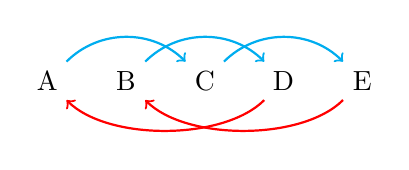
\begin{tikzpicture}
    \node(1) {A};
    \node[right of=1] (2) {B};
    \node[right of=2] (3) {C};
    \node[right of=3] (4) {D};
    \node[right of=4] (5) {E};
    \draw[->, thick]
    (1) edge[cyan, out=45, in=135, looseness=1,] (3)
    (2) edge[cyan, out=45, in=135, looseness=1,] (4)
    (3) edge[cyan, out=45, in=135, looseness=1,] (5)
    (4) edge[red, out=-135, in=-45, looseness=0.75,] (1)
    (5) edge[red, out=-135, in=-45, looseness=0.75,] (2)
;

\end{tikzpicture}
    \caption{Material transpositions}
    \label{fig:akasha-material-transposition-1}
\end{figure}

This operation is equivalent to +2 from the basic form with a modulus of five, such that materials transposed higher than the available 5 wrap back around to the beginning of the material set. The moments are repartitioned into new sections of different sizes:

\begin{table}[H]
    % \centering
    \resizebox{!}{40pt}{
\begin{tabular}{ c | c | c c c c c | c c | c c c}
 sections & ([04]) & [05] &  &  &  &  & [06] &  & [07] &  &  \\  
 moments & \textcolor{red}{13} & \textcolor{red}{14} & \textcolor{red}{15} & \textcolor{red}{16} & \textcolor{red}{17} & \textcolor{red}{18} & \textcolor{red}{19} & \textcolor{red}{20} & \textcolor{red}{21} & \textcolor{red}{22} & \textcolor{red}{23} \\
 measures & 59-61 & 62-70 & 71-93 & 94-98 & 99-103 & 104-112 & 113-151 &  & 152-161 & 162-173  &  174-186 \\  
 \midrule
materials &  &  &  &  &  & C &  &  & C &  &  \\  
 & C & D & D & E & C & D & E & A & A & C & B \\ 
 & D &  & E &  & E & E & A &  & B & B &  \\  
\end{tabular}
}
\caption{\textit{Akasha} moments, part 2}
    \label{tab:moments-2}
\end{table}

Transpositions are applied once more. Materials in blue represent materials which Bača replaces in a later step:

\begin{table}[H]
    % \centering
    \resizebox{!}{27.2pt}{
\begin{tabular}{ c | c c | c c c | c | c c c c | c}
 sections & ([07]) &  & [08] &  &  & [09] & [10] &  &  &  & [12] \\
 \midrule
 materials & &  &  &  &  & \textcolor{printBlue}{E} &  &  & \textcolor{printBlue}{E} &  &  \\  
&  E & A & A & B & E & \textcolor{printBlue}{A} & \textcolor{printBlue}{B} & \textcolor{printBlue}{C} & \textcolor{printBlue}{C} & \textcolor{printBlue}{E} & \textcolor{printBlue}{D} \\ 
&  A &  & B &  & B & \textcolor{printBlue}{B} & \textcolor{printBlue}{C} &  & \textcolor{printBlue}{D} & \textcolor{printBlue}{D} &  \\  
\end{tabular}
}
 \caption{\textit{Akasha} moments, part 3 (original)}
    \label{tab:moments-3-a}
\end{table}

The transpositions are applied once again and the moments are repartitioned:

\begin{table}[H]
    % \centering
    \resizebox{!}{40pt}{
\begin{tabular}{ c | c c c c | c c | c c | c c c}
sections & ([12]) &  &  &  & [13] &  & [14] &  & [15] &  &  \\  
moments &  \textcolor{red}{35} & \textcolor{red}{36} & \textcolor{red}{37} & \textcolor{red}{38} & \textcolor{red}{39} & \textcolor{red}{40} & \textcolor{red}{41} & \textcolor{red}{42} & \textcolor{red}{43} & \textcolor{red}{44} & \textcolor{red}{45} \\
measures & (265-333) &  &  &  & 334-339 &  & 340-368 &  & 369-393 &  &  \\
\midrule
materials &  &  &  &  &  & \colorbox{yellow}{B} &  &  & \colorbox{yellow}{B} &  &  \\  
& B & C & C & D & B & \colorbox{yellow}{C} & \colorbox{yellow}{D} & \colorbox{yellow}{E} & \colorbox{yellow}{E} & \colorbox{yellow}{B} & \colorbox{yellow}{A} \\ 
& C &  & D &  & D & \colorbox{yellow}{D} & \colorbox{yellow}{E} &  & \colorbox{yellow}{A} & \colorbox{yellow}{A} &  \\  
\end{tabular}
}
 \caption{\textit{Akasha} moments, part 4}
    \label{tab:moments-4}
\end{table}

Finally, the materials in sections 9-12 are replaced by their transpositional equivalents derived in figure \ref{tab:moments-4}, indicated in yellow:

\begin{table}[H]
    % \centering
    \resizebox{!}{40pt}{
\begin{tabular}{ c | c c | c c c | c | c c c c | c}
 sections & ([07]) &  & [08] &  &  & [09] & [10] &  &  &  & [12] \\  
 moments & \textcolor{red}{24} & \textcolor{red}{25} & \textcolor{red}{26} & \textcolor{red}{27} & \textcolor{red}{28} & \textcolor{red}{29} & \textcolor{red}{30} & \textcolor{red}{31} & \textcolor{red}{32} & \textcolor{red}{33} & \textcolor{red}{35} \\
 measures & 187-195 & 196-199 & 200-203 & 204-213 & 214-216 & 117-223 & 224-239 & 240-243 & 244-253 & 254-260 & 265-333 \\
 \midrule
 materials & &  &  &  &  & \colorbox{yellow}{B} &  &  & \colorbox{yellow}{B} &  &  \\  
&  E & A & A & B & E & \colorbox{yellow}{C} & \colorbox{yellow}{D} & \colorbox{yellow}{E} & \colorbox{yellow}{E} & \colorbox{yellow}{B} & \colorbox{yellow}{A} \\ 
&  A &  & B &  & B & \colorbox{yellow}{D} & \colorbox{yellow}{E} &  & \colorbox{yellow}{A} & \colorbox{yellow}{A} &  \\  
\end{tabular}
}
 \caption{\textit{Akasha} moments, part 3 (with substitution)}
    \label{tab:moments-3-b}
\end{table}

The sections represent distinct passages of compositional effort, ultimately forming the basis of \textit{Akasha}'s 15 sections. After the completion of the moment diagram (as attested by the version history of the section files found on GitHub\footnote{\url{https://github.com/}}), Bača added the opening gesture of material \boxed{\text{E}} to this structure, perhaps to soften the opening. Bača also inserted a section before what would originally have been called section eleven,\footnote{The inserted section eleven comprises moment 34 from measures 261-264 on material \boxed{\text{A}}, recollecting, as previously stated, the start of section six.} with an exact quotation of material found in section six. After designing this ordering of the materials, Bača then wrote an outline of the work, featuring written descriptions of each musical gesture. This storyboard describes the sequence of every event in the piece.

\section{Time Signature Series}

Time signature analysis reveals a pattern of alternation between two different types of time signature in the piece. The generative process for each series is defined; then, each series is rotated for every section of the piece at regular intervals of rotation. As described in Appendix \vref{helianthus}, Bača rotates the outer and inner layers as in \autoref{lst:sigs}, with reversed rotations of -1 and 1. Because helianthation produces a nested list of sublists, the section-specific time signature rotation refers to the sublist on which the time signatures begin. The other feature of the time signature series, common to Bača's other works, is monotonic increase of integers in each sublist.

\begin{lstlisting}[language=Python,frame=tb,caption={Definition of time signatures in \textit{Akasha}},label=lst:sigs]
def _time_signature_series():
    time_signature_series = dict()
    numerators = [[3, 3, 4, 5], [4, 6, 6]]
    groups = baca.sequence.helianthate(numerators, -1, 1)
    assert len(groups) == 24
    lengths = [len(_) for _ in groups]
    numerators = abjad.sequence.flatten(groups, depth=-1)
    _time_signatures = [abjad.TimeSignature((_, 4)) for _ in numerators]
    groups = abjad.sequence.partition_by_counts(_time_signatures, lengths)
    time_signature_series["A"] = groups
    numerators = [[3, 6, 7, 7], [4, 8, 9, 9], [3, 4]]
    groups = baca.sequence.helianthate(numerators, -1, 1)
    assert len(groups) == 36
    lengths = [len(_) for _ in groups]
    numerators = abjad.sequence.flatten(groups, depth=-1)
    _time_signatures = [abjad.TimeSignature((_, 8)) for _ in numerators]
    groups = abjad.sequence.partition_by_counts(_time_signatures, lengths)
    time_signature_series["B"] = groups
    return time_signature_series
\end{lstlisting}

\subsection{Time Signature Series A}

Time signature series A is defined as the sequence $[[3, 3, 4, 5], [4, 6, 6]]$ and its collection of helianthations, accumulated to identity. This series is used in sections 2, 4, 6, 7, 9, 10, 11, 13, and 14 of the piece. For each section, the series is rotated by 0, 3, 6, 9, 12, 15, 6, 18, and 21, representing a continuous rotation by three. Section eleven features a different rotation because this section flashes back to section six as an exact recurrence. The numbers produced by this series are treated as numerators of time signatures over denominators of \lilyText{4}.

\begin{lstlisting}[language=Python,frame=tb,caption={Enumeration of helianthated rotations of time signature series A},label=lst:sigs-a]
>>> numerators = [[3, 3, 4, 5], [4, 6, 6]]
>>> groups = baca.sequence.helianthate(numerators, -1, 1)
>>> partitions = abjad.sequence.partition_by_counts(groups, [2], cyclic=True)
>>> for partition in partitions:
...     print(partition)
...
[[3, 3, 4, 5], [4, 6, 6]]
[[6, 4, 6], [5, 3, 3, 4]]
[[4, 5, 3, 3], [6, 6, 4]]
[[4, 6, 6], [3, 4, 5, 3]]
[[3, 3, 4, 5], [6, 4, 6]]
[[6, 6, 4], [5, 3, 3, 4]]
[[4, 5, 3, 3], [4, 6, 6]]
[[6, 4, 6], [3, 4, 5, 3]]
[[3, 3, 4, 5], [6, 6, 4]]
[[4, 6, 6], [5, 3, 3, 4]]
[[4, 5, 3, 3], [6, 4, 6]]
[[6, 6, 4], [3, 4, 5, 3]]
\end{lstlisting}

\begin{table}[H]
    \centering
    \resizebox{\columnwidth}{!}{
    \begin{tabular}{ c c l }
 Section & Index of rotation & Time signatures \\ 
 \toprule
 2 & 0 & \lilyTimeSignature{3}{4}, \lilyTimeSignature{3}{4}, \lilyTimeSignature{4}{4}, \lilyTimeSignature{5}{4}, \lilyTimeSignature{4}{4}, \lilyTimeSignature{6}{4}, \lilyTimeSignature{6}{4}, \lilyTimeSignature{6}{4}, \lilyTimeSignature{4}{4}, \lilyTimeSignature{6}{4}, \lilyTimeSignature{5}{4}, \lilyTimeSignature{3}{4} \\  
 % \midrule
 \vspace{0.25mm} \\
 4 & 3 & \lilyTimeSignature{6}{4}, \lilyTimeSignature{4}{4}, \lilyTimeSignature{6}{4}, \lilyTimeSignature{6}{4}, \lilyTimeSignature{6}{4}, \lilyTimeSignature{4}{4}, \lilyTimeSignature{3}{4}, \lilyTimeSignature{4}{4}, \lilyTimeSignature{5}{4}, \lilyTimeSignature{3}{4}, \lilyTimeSignature{3}{4}, \lilyTimeSignature{3}{4}, \lilyTimeSignature{4}{4}, \lilyTimeSignature{5}{4}, \lilyTimeSignature{4}{4}, \lilyTimeSignature{6}{4}, \lilyTimeSignature{6}{4} \\ 
 % \midrule
 \vspace{0.25mm} \\
 6 & 6 & \lilyTimeSignature{4}{4}, \lilyTimeSignature{6}{4}, \lilyTimeSignature{6}{4}, \lilyTimeSignature{5}{4}, \lilyTimeSignature{3}{4}, \lilyTimeSignature{3}{4}, \lilyTimeSignature{4}{4}, \lilyTimeSignature{4}{4}, \lilyTimeSignature{5}{4}, \lilyTimeSignature{3}{4}, \lilyTimeSignature{3}{4}, \lilyTimeSignature{6}{4}, \lilyTimeSignature{4}{4}, \lilyTimeSignature{6}{4}, \lilyTimeSignature{6}{4}, \lilyTimeSignature{6}{4}, \lilyTimeSignature{4}{4}, \lilyTimeSignature{3}{4}, \lilyTimeSignature{4}{4}, \lilyTimeSignature{5}{4}, \lilyTimeSignature{3}{4}, \lilyTimeSignature{3}{4}, \lilyTimeSignature{3}{4}, \lilyTimeSignature{4}{4}, \lilyTimeSignature{5}{4}, \lilyTimeSignature{4}{4}, \lilyTimeSignature{6}{4}, \lilyTimeSignature{6}{4}, \lilyTimeSignature{6}{4}, \lilyTimeSignature{4}{4}, \lilyTimeSignature{6}{4}, \lilyTimeSignature{5}{4}, \lilyTimeSignature{3}{4}, \lilyTimeSignature{3}{4} \\ 
  % \midrule
  \vspace{0.25mm} \\
 7 & 9 & \lilyTimeSignature{3}{4}, \lilyTimeSignature{4}{4}, \lilyTimeSignature{5}{4}, \lilyTimeSignature{3}{4}, \lilyTimeSignature{3}{4}, \lilyTimeSignature{3}{4}, \lilyTimeSignature{4}{4}, \lilyTimeSignature{5}{4}, \lilyTimeSignature{6}{4}, \lilyTimeSignature{6}{4}, \lilyTimeSignature{4}{4}, \lilyTimeSignature{4}{4}, \lilyTimeSignature{6}{4}, \lilyTimeSignature{6}{4}, \lilyTimeSignature{5}{4}, \lilyTimeSignature{3}{4}, \lilyTimeSignature{3}{4}, \lilyTimeSignature{4}{4}, \lilyTimeSignature{4}{4}, \lilyTimeSignature{5}{4}, \lilyTimeSignature{3}{4}, \lilyTimeSignature{3}{4}, \lilyTimeSignature{6}{4}, \lilyTimeSignature{4}{4}, \lilyTimeSignature{6}{4}, \lilyTimeSignature{6}{4}, \lilyTimeSignature{6}{4}, \lilyTimeSignature{4}{4}, \lilyTimeSignature{3}{4}, \lilyTimeSignature{4}{4}, \lilyTimeSignature{5}{4}, \lilyTimeSignature{3}{4}, \lilyTimeSignature{3}{4}, \lilyTimeSignature{3}{4}, \lilyTimeSignature{4}{4}, \lilyTimeSignature{5}{4}, \lilyTimeSignature{4}{4}, \lilyTimeSignature{6}{4}, \lilyTimeSignature{6}{4}, \lilyTimeSignature{6}{4} \\ 
  % \midrule
  \vspace{0.25mm} \\
 9 & 12 & \lilyTimeSignature{4}{4}, \lilyTimeSignature{5}{4}, \lilyTimeSignature{3}{4}, \lilyTimeSignature{3}{4}, \lilyTimeSignature{4}{4} \\ 
  % \midrule
  \vspace{0.25mm} \\
 10 & 15 & \lilyTimeSignature{6}{4}, \lilyTimeSignature{4}{4}, \lilyTimeSignature{6}{4}, \lilyTimeSignature{6}{4}, \lilyTimeSignature{6}{4}, \lilyTimeSignature{4}{4}, \lilyTimeSignature{5}{4}, \lilyTimeSignature{3}{4}, \lilyTimeSignature{3}{4}, \lilyTimeSignature{4}{4}, \lilyTimeSignature{4}{4}, \lilyTimeSignature{5}{4}, \lilyTimeSignature{3}{4}, \lilyTimeSignature{3}{4}, \lilyTimeSignature{4}{4}, \lilyTimeSignature{6}{4}, \lilyTimeSignature{6}{4}, \lilyTimeSignature{6}{4}, \lilyTimeSignature{4}{4}, \lilyTimeSignature{6}{4}, \lilyTimeSignature{3}{4}, \lilyTimeSignature{4}{4}, \lilyTimeSignature{5}{4}, \lilyTimeSignature{3}{4}, \lilyTimeSignature{3}{4}, \lilyTimeSignature{3}{4}, \lilyTimeSignature{4}{4}, \lilyTimeSignature{5}{4}, \lilyTimeSignature{6}{4}, \lilyTimeSignature{6}{4}, \lilyTimeSignature{4}{4}, \lilyTimeSignature{4}{4}, \lilyTimeSignature{6}{4} \\ 
  % \midrule
  \vspace{0.25mm} \\
 11 & 6 & \lilyTimeSignature{4}{4}, \lilyTimeSignature{6}{4}, \lilyTimeSignature{6}{4} \\ 
  % \midrule
  \vspace{0.25mm} \\
 13 & 18 & \lilyTimeSignature{4}{4}, \lilyTimeSignature{6}{4}, \lilyTimeSignature{6}{4}, \lilyTimeSignature{3}{4} \\ 
  % \midrule
  \vspace{0.25mm} \\
 14 & 21 & \lilyTimeSignature{5}{4}, \lilyTimeSignature{3}{4}, \lilyTimeSignature{3}{4}, \lilyTimeSignature{4}{4}, \lilyTimeSignature{4}{4}, \lilyTimeSignature{5}{4}, \lilyTimeSignature{3}{4}, \lilyTimeSignature{3}{4}, \lilyTimeSignature{6}{4}, \lilyTimeSignature{6}{4}, \lilyTimeSignature{4}{4}, \lilyTimeSignature{4}{4}, \lilyTimeSignature{6}{4}, \lilyTimeSignature{6}{4}, \lilyTimeSignature{3}{4}, \lilyTimeSignature{4}{4}, \lilyTimeSignature{5}{4}, \lilyTimeSignature{3}{4}, \lilyTimeSignature{3}{4}, \lilyTimeSignature{3}{4}, \lilyTimeSignature{4}{4}, \lilyTimeSignature{5}{4}, \lilyTimeSignature{6}{4}, \lilyTimeSignature{4}{4}, \lilyTimeSignature{6}{4}, \lilyTimeSignature{6}{4}, \lilyTimeSignature{6}{4}, \lilyTimeSignature{4}{4} \\ 
 \bottomrule
\end{tabular}
}
    \caption{Time signature series A}
    \label{fig:series-a-table}
\end{table}

\subsection{Time Signature Series B}

Time signature series B is defined as the sequence $[[3, 6, 7, 7], [4, 8, 9, 9], [3, 4]]$ and its sequence of helianthations, accumulated to identity with denominators of \lilyText{8}. This time signature series is used in sections 1, 3, 5, 8, 12, 15 with rotations of 0, 6, 12, 18, 24, 30, respectively.

\begin{lstlisting}[language=Python,frame=tb,caption={Enumeration of helianthated rotations of time signature series B},label=lst:sigs-b]
>>> numerators = [[3, 6, 7, 7], [4, 8, 9, 9], [3, 4]]
>>> groups = baca.sequence.helianthate(numerators, -1, 1)
>>> partitions = abjad.sequence.partition_by_counts(groups, [3], cyclic=True)
>>> for partition in partitions:
...     print(partition)
...
[[3, 6, 7, 7], [4, 8, 9, 9], [3, 4]]
[[9, 4, 8, 9], [4, 3], [7, 3, 6, 7]]
[[3, 4], [7, 7, 3, 6], [9, 9, 4, 8]]
[[6, 7, 7, 3], [8, 9, 9, 4], [4, 3]]
[[4, 8, 9, 9], [3, 4], [3, 6, 7, 7]]
[[4, 3], [7, 3, 6, 7], [9, 4, 8, 9]]
[[7, 7, 3, 6], [9, 9, 4, 8], [3, 4]]
[[8, 9, 9, 4], [4, 3], [6, 7, 7, 3]]
[[3, 4], [3, 6, 7, 7], [4, 8, 9, 9]]
[[7, 3, 6, 7], [9, 4, 8, 9], [4, 3]]
[[9, 9, 4, 8], [3, 4], [7, 7, 3, 6]]
[[4, 3], [6, 7, 7, 3], [8, 9, 9, 4]]
\end{lstlisting}

\begin{table}[H]
    \centering
    \resizebox{\columnwidth}{!}{
    \begin{tabular}{ c c l }
 Section & Index of rotation & Time signatures \\ 
 \toprule
 1 & 0 & \lilyTimeSignature{3}{8}, \lilyTimeSignature{6}{8} \\  
 % \midrule
 \vspace{0.25mm} \\
 3 & 6 & \lilyTimeSignature{9}{8}, \lilyTimeSignature{9}{8}, \lilyTimeSignature{4}{8}, \lilyTimeSignature{8}{8}, \lilyTimeSignature{3}{8}, \lilyTimeSignature{4}{8}, \lilyTimeSignature{7}{8}, \lilyTimeSignature{7}{8} \\
 % \midrule
 \vspace{0.25mm} \\
 5 & 12 & \lilyTimeSignature{3}{8}, \lilyTimeSignature{4}{8}, \lilyTimeSignature{3}{8}, \lilyTimeSignature{6}{8}, \lilyTimeSignature{7}{8}, \lilyTimeSignature{7}{8}, \lilyTimeSignature{4}{8}, \lilyTimeSignature{8}{8}, \lilyTimeSignature{9}{8}, \lilyTimeSignature{9}{8}, \lilyTimeSignature{7}{8}, \lilyTimeSignature{3}{8}, \lilyTimeSignature{6}{8}, \lilyTimeSignature{7}{8}, \lilyTimeSignature{9}{8}, \lilyTimeSignature{4}{8}, \lilyTimeSignature{8}{8}, \lilyTimeSignature{9}{8}, \lilyTimeSignature{4}{8}, \lilyTimeSignature{3}{8}, \lilyTimeSignature{9}{8}, \lilyTimeSignature{9}{8}, \lilyTimeSignature{4}{8}, \lilyTimeSignature{8}{8}, \lilyTimeSignature{3}{8}, \lilyTimeSignature{4}{8}, \lilyTimeSignature{7}{8}, \lilyTimeSignature{7}{8}, \lilyTimeSignature{3}{8}, \lilyTimeSignature{6}{8}, \lilyTimeSignature{4}{8}, \lilyTimeSignature{3}{8}, \lilyTimeSignature{6}{8}, \lilyTimeSignature{7}{8}, \lilyTimeSignature{7}{8}, \lilyTimeSignature{3}{8}, \lilyTimeSignature{8}{8}, \lilyTimeSignature{9}{8}, \lilyTimeSignature{9}{8}, \lilyTimeSignature{4}{8}, \\
 & & \lilyTimeSignature{3}{8}, \lilyTimeSignature{6}{8}, \lilyTimeSignature{7}{8}, \lilyTimeSignature{7}{8} \\
 % \midrule
 \vspace{0.25mm} \\
 8 & 18 & \lilyTimeSignature{7}{8}, \lilyTimeSignature{7}{8}, \lilyTimeSignature{3}{8}, \lilyTimeSignature{6}{8}, \lilyTimeSignature{9}{8}, \lilyTimeSignature{9}{8}, \lilyTimeSignature{4}{8}, \lilyTimeSignature{8}{8}, \lilyTimeSignature{3}{8}, \lilyTimeSignature{4}{8}, \lilyTimeSignature{8}{8}, \lilyTimeSignature{9}{8}, \lilyTimeSignature{9}{8}, \lilyTimeSignature{4}{8}, \lilyTimeSignature{4}{8}, \lilyTimeSignature{3}{8} \\
 % \midrule
 \vspace{0.25mm} \\
 12 & 24 & \lilyTimeSignature{4}{8}, \lilyTimeSignature{8}{8}, \lilyTimeSignature{9}{8}, \lilyTimeSignature{9}{8}, \lilyTimeSignature{3}{8}, \lilyTimeSignature{4}{8}, \lilyTimeSignature{3}{8}, \lilyTimeSignature{6}{8}, \lilyTimeSignature{7}{8}, \lilyTimeSignature{7}{8}, \lilyTimeSignature{4}{8}, \lilyTimeSignature{3}{8}, \lilyTimeSignature{7}{8}, \lilyTimeSignature{3}{8}, \lilyTimeSignature{6}{8}, \lilyTimeSignature{7}{8}, \lilyTimeSignature{9}{8}, \lilyTimeSignature{4}{8}, \lilyTimeSignature{8}{8}, \lilyTimeSignature{9}{8}, \lilyTimeSignature{7}{8}, \lilyTimeSignature{7}{8}, \lilyTimeSignature{3}{8}, \lilyTimeSignature{6}{8}, \lilyTimeSignature{9}{8}, \lilyTimeSignature{9}{8}, \lilyTimeSignature{4}{8}, \lilyTimeSignature{8}{8}, \lilyTimeSignature{3}{8}, \lilyTimeSignature{4}{8}, \lilyTimeSignature{8}{8}, \lilyTimeSignature{9}{8}, \lilyTimeSignature{9}{8}, \lilyTimeSignature{4}{8}, \lilyTimeSignature{4}{8}, \lilyTimeSignature{3}{8}, \lilyTimeSignature{6}{8}, \lilyTimeSignature{7}{8}, \lilyTimeSignature{7}{8}, \lilyTimeSignature{3}{8}, \\
 & & \lilyTimeSignature{3}{8}, \lilyTimeSignature{4}{8}, \lilyTimeSignature{3}{8}, \lilyTimeSignature{6}{8}, \lilyTimeSignature{7}{8}, \lilyTimeSignature{7}{8}, \lilyTimeSignature{4}{8}, \lilyTimeSignature{8}{8}, \lilyTimeSignature{9}{8}, \lilyTimeSignature{9}{8}, \lilyTimeSignature{7}{8}, \lilyTimeSignature{3}{8}, \lilyTimeSignature{6}{8}, \lilyTimeSignature{7}{8}, \lilyTimeSignature{9}{8}, \lilyTimeSignature{4}{8}, \lilyTimeSignature{8}{8}, \lilyTimeSignature{9}{8}, \lilyTimeSignature{4}{8}, \lilyTimeSignature{3}{8}, \lilyTimeSignature{9}{8}, \lilyTimeSignature{9}{8}, \lilyTimeSignature{4}{8}, \lilyTimeSignature{8}{8} \\
 % \midrule
 \vspace{0.25mm} \\
 15 & 30 & \lilyTimeSignature{3}{8}, \lilyTimeSignature{4}{8}, \lilyTimeSignature{7}{8}, \lilyTimeSignature{7}{8}, \lilyTimeSignature{3}{8}, \lilyTimeSignature{6}{8}, \lilyTimeSignature{9}{8}, \lilyTimeSignature{9}{8}, \lilyTimeSignature{4}{8}, \lilyTimeSignature{8}{8}, \lilyTimeSignature{6}{8}, \lilyTimeSignature{7}{8}, \lilyTimeSignature{7}{8}, \lilyTimeSignature{3}{8}, \lilyTimeSignature{8}{8}, \lilyTimeSignature{9}{8}, \lilyTimeSignature{9}{8}, \lilyTimeSignature{4}{8}, \lilyTimeSignature{4}{8}, \lilyTimeSignature{3}{8}, \lilyTimeSignature{4}{8}, \lilyTimeSignature{8}{8}, \lilyTimeSignature{9}{8}, \lilyTimeSignature{9}{8} \\
 \bottomrule
\end{tabular}
}
    \caption{Time signature series B}
    \label{fig:series-b-table}
\end{table}

After defining the process by which time signatures are arranged in each section, Bača chooses the number of measures for each section. Some measures are selected to be a silent grand pause; these are inserted between time signatures, visually compressed, and given a fermata.

\section{Sections 1-6}

Here I describe the opening 6 sections of \textit{Akasha}.

\begin{table}[H]
    % \centering
    \begin{tabular}{c|l}
        Section & Measures \\
        \toprule
        1 & 1-3 \\
        2 & 4-23 \\ 
        3 & 24-34 \\ 
        4 & 35-61 \\ 
        5 & 62-112 \\ 
        6 & 113-151 \\ 
    \end{tabular}
    \caption{Sections 1-6 in \textit{Akasha}}
    \label{tab:akasha-1-6-measures}
\end{table}

\subsection{Section 1}

The work begins with a sputtering, interruptive exposition where the different materials are fairly easy to distinguish from one another. Section 1 consists of a single note of the viola bowing on the bridge at \lilyDynamics{mf}, followed by a very long fermata. %This insertion causes the work to begin with material \boxed{\text{E}} instead of the originally planned \boxed{\text{A}}.

% \begin{figure}[H]
%     \includegraphics[scale=0.75]{lilypond/akasha_01.pdf}
%     \caption{Section 1 of \textit{Akasha} Annotated}
%     \label{fig:akasha-1}
% \end{figure}

\subsection{Section 2}

The \textbf{2\textsuperscript{nd}} moment, in measures 4-8, corresponds to materials \boxed{\text{AB}} interpreted as a sequential statement. The cello, playing \boxed{\text{B}}, has rhythms derived from a talea of durations $\frac{7}{16}$, $\frac{1}{16}$, $\frac{10}{16}$, and $\frac{2}{16}$:

\begin{figure}[H]
    \includegraphics{lilypond/section_2/akasha_cello_1.pdf}
    \caption{Cello; measures 4-5; score}
    \label{fig:cello-talea}
\end{figure}

The rhythms of the second violin and viola, playing \boxed{\text{A}}, are also derived from a talea of 32\textsuperscript{nd} notes:

\setcounter{figure}{7}
\setcounter{subFigure}{1}
\renewcommand{\thefigure}{\thechapter.\arabic{figure}.\alph{subFigure}}
\begin{figure}[H]
    \includegraphics{lilypond/section_2/akasha_violin_viola_step_1.pdf}
    \caption{Violin 2 and viola; measure 7; stage 1}
    \label{fig:violin-viola-talea-1}
\end{figure}

One extra count is included in each quarter note subdivision:

% \setcounter{figure}{7}
% \setcounter{subFigure}{2}
% \begin{figure}[H]
%     \includegraphics{lilypond/section_2/akasha_violin_viola_step_2.pdf}
%     \caption{Violin 2 and viola; measure 7; stage 2}
%     \label{fig:violin-viola-talea-2}
% \end{figure}

% The measure is subdivided into quarter note durations:

\setcounter{figure}{7}
\setcounter{subFigure}{2}
\begin{figure}[H]
    \includegraphics{lilypond/section_2/akasha_violin_viola_step_3.pdf}
    \caption{Violin 2 and viola; measure 7; stage 2}
    \label{fig:violin-viola-talea-3}
\end{figure}

Over a period of 36 notes, only attacks 0, 1, 2, 12, 13, 21, 31, 32, and 33 are heard:

\setcounter{figure}{7}
\setcounter{subFigure}{3}
\begin{figure}[H]
    \includegraphics{lilypond/section_2/akasha_violin_viola_step_4.pdf}
    \caption{Violin 2 and viola; measure 7; stage 3}
    \label{fig:violin-viola-talea-4}
\end{figure}

In the case of the second violin, all tuplets except for the first two are silenced, while the viola silences all but the last:

\setcounter{figure}{7}
\setcounter{subFigure}{4}
\begin{figure}[H]
    \includegraphics{lilypond/section_2/akasha_violin_viola_step_5.pdf}
    \caption{Violin 2 and viola; measure 7; stage 4}
    \label{fig:violin-viola-talea-5}
\end{figure}

Empty tuplets are respelled as rests:

\setcounter{figure}{7}
\setcounter{subFigure}{5}
\begin{figure}[H]
    \includegraphics{lilypond/section_2/akasha_violin_viola_step_5_score.pdf}
    \caption{Violin 2 and viola; measure 7; score}
    \label{fig:violin-viola-talea-5-score}
\end{figure}

The \textbf{3\textsuperscript{rd}} moment, in measures 9-13, corresponds to the materials \boxed{\text{B(A)}} interpreted as a sequential statement, with an overlap. Here material \boxed{\text{A}} has been reintroduced despite the original map containing only \boxed{\text{B}}. The \boxed{\text{B}} rhythms in both violins and the viola are produced with the same methodology as the cello (figure \ref{fig:cello-talea}), only with substituted duration numerators and occasional rotation. The talea consists of durations $\frac{4}{16}$, $\frac{14}{16}$, $\frac{4}{16}$, $\frac{6}{16}$, $\frac{18}{16}$:

\setcounter{figure}{8}
\setcounter{subFigure}{1}
% \renewcommand{\thefigure}{\thechapter.\arabic{figure}}
\begin{figure}[H]
% \resizebox{\columnwidth}{!}{
    \includegraphics{lilypond/section_2/polyphony_1.pdf}
    % }
    \caption{Violins and viola; measures 9-10; stage 1}
    \label{fig:polyphony-talea-1}
\end{figure}

Violin 1 silences all notes except those at index 0, 1, 2. Violin 2 silences all notes except those at index 2, 3, 4. The viola silences all notes except those at index 1, 2, 3. This produces a slightly staggered entrance and exit of each voice, but preserves rhythmic unison:

\setcounter{figure}{8}
\setcounter{subFigure}{2}
\begin{figure}[H]
% \resizebox{\columnwidth}{!}{
    \includegraphics{lilypond/section_2/polyphony_2.pdf}
    % }
    \caption{Violins and viola; measures 9-10; score}
    \label{fig:polyphony-talea-2}
\end{figure}

After the fermata (m. 11), \boxed{\text{B}} is moved to the lower trio of violin 2, viola, and cello, with a rotation of -2, producing $\frac{4}{16}$, $\frac{6}{16}$, $\frac{18}{16}$, $\frac{4}{16}$, $\frac{14}{16}$:

\setcounter{figure}{9}
\setcounter{subFigure}{1}
\begin{figure}[H]
% \resizebox{\columnwidth}{!}{
    \includegraphics{lilypond/section_2/polyphony_3.pdf}
    % }
    \caption{Violin 2, viola, and cello; measure 12; stage 1}
    \label{fig:polyphony-talea-3}
\end{figure}

Violin 2 silences all but indices 1, 2, and 3. The viola, also with a rotation of -2, silences all but indices 2, 3, and 4. The cello, with a rotation of -2, silences all but indices 0, 1, and 2. This produces the same effect of staggered entrances and exits with coincident attacks:

\setcounter{figure}{9}
\setcounter{subFigure}{2}
\begin{figure}[H]
% \resizebox{\columnwidth}{!}{
    \includegraphics{lilypond/section_2/polyphony_4.pdf}
    % }
    \caption{Violin 2, viola, and cello; measure 12; score}
    \label{fig:polyphony-talea-4}
\end{figure}

The first violin, now playing material \boxed{\text{A}}, produces the same rhythms as the first appearance of \boxed{\text{A}} in the second violin and viola:

\setcounter{figure}{10}
\setcounter{subFigure}{1}
\begin{figure}[H]
% \resizebox{\columnwidth}{!}{
    \includegraphics{lilypond/section_2/gettato_3.pdf}
    % }
    \caption{Violin 1; measure 12; stage 1}
    \label{fig:gettato-v1-1}
\end{figure}

All but the last two tuplets are silenced:

\setcounter{figure}{10}
\setcounter{subFigure}{2}
\begin{figure}[H]
% \resizebox{\columnwidth}{!}{
    \includegraphics{lilypond/section_2/gettato_4.pdf}
    % }
    \caption{Violin 1; measure 12; stage 2}
    \label{fig:gettato-v1-4}
\end{figure}

Empty tuplets are respelled as rests:

\setcounter{figure}{10}
\setcounter{subFigure}{3}
\begin{figure}[H]
% \resizebox{\columnwidth}{!}{
    \includegraphics{lilypond/section_2/gettato_4_score.pdf}
    % }
    \caption{Violin 1; measure 12; score}
    \label{fig:gettato-v1-4-score}
\end{figure}

The \textbf{4\textsuperscript{th}} moment, in measures 14-19, corresponds to the materials \boxed{\text{BC}} interpreted as an overlapping statement. Material \boxed{\text{B}} in the viola, with a rotation of -4 is accompanied by the cello, with a rotation of -6. This produces a duet with individual taleas of ($\frac{18}{16}$, $\frac{4}{16}$, $\frac{14}{16}$, $\frac{4}{16}$, $\frac{6}{16}$) and ($\frac{14}{16}$, $\frac{4}{16}$, $\frac{6}{16}$, $\frac{18}{16}$, $\frac{4}{16}$):

\setcounter{figure}{11}
\setcounter{subFigure}{1}
\renewcommand{\thefigure}{\thechapter.\arabic{figure}}
\begin{figure}[H]
% \resizebox{\columnwidth}{!}{
    \includegraphics{lilypond/section_2/duet_1.pdf}
    % }
    \caption{Viola and cello; measures 14-16; score}
    \label{fig:duet-1}
\end{figure}

This begins the development of a continuous rotation pattern, where each appearance of material \boxed{\text{B}} in the viola is rotated two positions to the left, and the cello is rotated four positions to the left. After the fermata, the viola and cello rhythms are rotated to their final position of -8 and -10 respectively. This produces a duet with individual taleas of ($\frac{6}{16}$, $\frac{18}{16}$, $\frac{4}{16}$, $\frac{14}{16}$, $\frac{4}{16}$) and ($\frac{4}{16}$, $\frac{14}{16}$, $\frac{4}{16}$, $\frac{6}{16}$, $\frac{18}{16}$):

\setcounter{figure}{12}
\begin{figure}[H]
% \resizebox{\columnwidth}{!}{
    \includegraphics{lilypond/section_2/duet_2.pdf}
    % }
    \caption{Viola and cello; measure 18; score}
    \label{fig:duet-2}
\end{figure}

As for the violins' \boxed{\text{C}} material, the accelerandi\footnote{For a description of the accelerando interpolation process, see \vref{rmakers}.} alternates between interpolations from $\frac{1}{2}$ to $\frac{1}{8}$ and $\frac{1}{8}$ to $\frac{1}{2}$. The total duration of the musical event is factored into the interpolation equation and the resulting accelerandi alternate between one measure and two measures in duration. Interpolations from short durations to longer durations are front-loaded to produce more attacks in a rallantando than an accelerando:

\setcounter{figure}{13}
\setcounter{subFigure}{1}
\renewcommand{\thefigure}{\thechapter.\arabic{figure}.\alph{subFigure}}
\begin{figure}[H]
% \resizebox{\columnwidth}{!}{
    \includegraphics{lilypond/section_2/acc_1.pdf}
    % }
    \caption{Violins; measures 14-16; stage 1}
    \label{fig:accelerando-1}
\end{figure}

The first violin silences all attacks except for -11, -10, -8, -6, -4, -2, and -1. The second violin's rhythm reverses the ordering of the accelerando/rallantando gestures and silences all but attacks -10, -8, -7, -5, -3, -2, and -1:

\setcounter{figure}{13}
\setcounter{subFigure}{2}
\begin{figure}[H]
% \resizebox{\columnwidth}{!}{
    \includegraphics{lilypond/section_2/acc_2.pdf}
    % }
    \caption{Violins; measures 14-16; stage 2}
    \label{fig:accelerando-2}
\end{figure}

Empty tuplets are respelled as rests:

\setcounter{figure}{13}
\setcounter{subFigure}{3}
\begin{figure}[H]
% \resizebox{\columnwidth}{!}{
    \includegraphics{lilypond/section_2/acc_2_score.pdf}
    % }
    \caption{Violins; measures 14-16; score}
    \label{fig:accelerando-2-score}
\end{figure}

Despite sharing nearly identical rest-forcing patterns, the opposing accelerando directions result in a lack of coincident attacks. In measure 18,\footnote{Fermatas are numbered as measures in the score.} the violins produce accelerandi identical to the previous measures, but revealing previously silenced opening gestures:

\setcounter{figure}{14}
\setcounter{subFigure}{1}
\begin{figure}[H]
% \resizebox{\columnwidth}{!}{
    \includegraphics{lilypond/section_2/acc_3.pdf}
    % }
    \caption{Violins; measure 18; stage 1}
    \label{fig:accelerando-3}
\end{figure}

Violin 1 silences all but 0, 2, 3, and -1, while violin 2 silences all but 0, 1, 4, and -1:

\setcounter{figure}{14}
\setcounter{subFigure}{2}
\renewcommand{\thefigure}{\thechapter.\arabic{figure}.\alph{subFigure}}
\begin{figure}[H]
% \resizebox{\columnwidth}{!}{
    \includegraphics{lilypond/section_2/acc_4.pdf}
    % }
    \caption{Violins; measure 18; score}
    \label{fig:accelerando-4}
\end{figure}

The \textbf{5\textsuperscript{th}} moment, in measures 20-21, develops material \boxed{\text{C}}. The violins play alone, with identical rhythms, but with a reversal of roles. Both violins silence all notes except those at indices 0, 2, and -1:

% \begin{figure}[H]
% % \resizebox{\columnwidth}{!}{
%     \includegraphics{lilypond/section_2/acc_5.pdf}
%     % }
%     \caption{Accelerando 5}
%     \label{fig:accelerando-5}
% \end{figure}

\setcounter{figure}{15}
\setcounter{subFigure}{0}
\renewcommand{\thefigure}{\thechapter.\arabic{figure}}
\begin{figure}[H]
% \resizebox{\columnwidth}{!}{
    \includegraphics{lilypond/section_2/acc_6.pdf}
    % }
    \caption{Violins; measure 20; score}
    \label{fig:accelerando-6}
\end{figure}

The \textbf{6\textsuperscript{th}} moment, in measures 22-23, interprets materials \boxed{\text{AC}} as a concurrent statement. Violin 2 uses the ritardando pattern with silences applied to all but 0, 1, -1:

\setcounter{figure}{16}
\begin{figure}[H]
% \resizebox{\columnwidth}{!}{
    \includegraphics{lilypond/section_2/acc_8.pdf}
    % }
    \caption{Violin 2; measure 22; score}
    \label{fig:accelerando-8}
\end{figure}

The cello takes up the 32\textsuperscript{nd}-note rhythms described above:

\setcounter{figure}{17}
\setcounter{subFigure}{1}
\renewcommand{\thefigure}{\thechapter.\arabic{figure}.\alph{subFigure}}
\begin{figure}[H]
% \resizebox{\columnwidth}{!}{
    \includegraphics{lilypond/section_2/gett_1.pdf}
    % }
    \caption{Cello; measure 22; stage 1}
    \label{fig:final-gett-1}
\end{figure}

The first and last tuplets are silenced:

\setcounter{figure}{17}
\setcounter{subFigure}{2}
\begin{figure}[H]
% \resizebox{\columnwidth}{!}{
    \includegraphics{lilypond/section_2/gett_2.pdf}
    % }
    \caption{Cello; measure 22; stage 2}
    \label{fig:final-gett-2}
\end{figure}

Empty tuplets are respelled as rests:

\setcounter{figure}{17}
\setcounter{subFigure}{3}
\begin{figure}[H]
% \resizebox{\columnwidth}{!}{
    \includegraphics{lilypond/section_2/gett_2_score.pdf}
    % }
    \caption{Cello; measure 22; score}
    \label{fig:final-gett-2-score}
\end{figure}

An examination of the pitch content of this section of the score reveals characteristic harmonic traits associated with each material. \boxed{\text{A}} uses semitones with a tendency toward neighbor-note motion. \boxed{\text{B}} makes use of quarter tones and mostly stepwise motion with contrary voice-leading. \boxed{\text{C}} takes the form of a highly slowed-down trill, so each voice only oscillates between two pitches. This version of the pitch material of \boxed{\text{C}} produces a whole-tone effect.

% \begin{figure}[H]
% \resizebox{\columnwidth}{!}{
%     \includegraphics{lilypond/akasha_02.pdf}
%     }
%     \caption{Section 2 of \textit{Akasha} Annotated}
%     \label{fig:akasha-2}
% \end{figure}

\subsection{Section 3}

The \textbf{7\textsuperscript{th}} moment, in measures 24-32, deploys the compound material \boxed{\text{ABC}}. Violin 1 performs an accelerando from material \boxed{\text{C}} on single measures. All notes are silenced except 0, 2, and 3:

\setcounter{figure}{18}
\setcounter{subFigure}{0}
\renewcommand{\thefigure}{\thechapter.\arabic{figure}}
\begin{figure}[H]
% \resizebox{\columnwidth}{!}{
    \includegraphics{lilypond/section_3/accel_1.pdf}
    % }
    \caption{Violin 1; measure 24; score}
    \label{fig:section-3-accel}
\end{figure}

The rhythm of \boxed{\text{B}} material is derived from the previous rhythms in violin 2 and in the viola with a rotation of -2 and silences for the first two note durations. This produces a duet of individual taleas of ($\frac{4}{16}$, $\frac{14}{16}$, $\frac{4}{16}$, $\frac{6}{16}$, $\frac{18}{16}$) and ($\frac{4}{16}$, $\frac{6}{16}$, $\frac{18}{16}$, $\frac{4}{16}$, $\frac{14}{16}$):

\setcounter{figure}{19}
\begin{figure}[H]
% \resizebox{\columnwidth}{!}{
    \includegraphics{lilypond/section_3/section_3_polyphony_1.pdf}
    % }
    \caption{Violin 2 and viola; measures 24-26; score}
    \label{fig:section-3-accel-2}
\end{figure}

The cello's first, four-measure statement of \boxed{\text{A}} deploys a variation on the 32\textsuperscript{nd}-note rhythms developed in section two. These rhythms are made through the creation of two patterns: one with indices 0, 1, 2, 3 with a period of 12 and another with the same indices with a period of 20:

\setcounter{figure}{20}
\setcounter{subFigure}{1}
\renewcommand{\thefigure}{\thechapter.\arabic{figure}.\alph{subFigure}}
\begin{figure}[H]
% \resizebox{\columnwidth}{!}{
    \includegraphics{lilypond/section_3/section_3_pattern_1.pdf}
    % }
    \caption{Cello; measures 24-27; stage 1; pattern 1}
    \label{fig:section-3-pattern-1}
\end{figure}

\setcounter{figure}{20}
\setcounter{subFigure}{2}
\begin{figure}[H]
% \resizebox{\columnwidth}{!}{
    \includegraphics{lilypond/section_3/section_3_pattern_2.pdf}
    % }
    \caption{Cello; measures 24-27; stage 1; pattern 2}
    \label{fig:section-3-pattern-2}
\end{figure}

The union of these patterns is taken:

\setcounter{figure}{20}
\setcounter{subFigure}{3}
\begin{figure}[H]
% \resizebox{\columnwidth}{!}{
    \includegraphics{lilypond/section_3/section_3_pattern_intersection.pdf}
    % }
    \caption{Cello; measures 24-27; stage 2}
    \label{fig:section-3-pattern-intersection}
\end{figure}

The union is inverted, such that notes become rests and rests become notes:

\setcounter{figure}{20}
\setcounter{subFigure}{4}
\begin{figure}[H]
% \resizebox{\columnwidth}{!}{
    \includegraphics{lilypond/section_3/section_3_inverted_intersection.pdf}
    % }
    \caption{Cello; measures 24-27; stage 3}
    \label{fig:section-3-inverted-intersection}
\end{figure}

Extra counts are cyclically applied to each quarter note subdivision with a pattern of $[1, 1, 0, 2]$:

% \begin{figure}[H]
% % \resizebox{\columnwidth}{!}{
%     \includegraphics{lilypond/section_3/section_3_extra_counts_pattern.pdf}
%     % }
%     \caption{Cello; measures 24-27; stage 4}
%     \label{fig:section-3-pattern-extra-counts}
% \end{figure}

% The measures are subdivided into quarter notes:

\setcounter{figure}{20}
\setcounter{subFigure}{5}
\begin{figure}[H]
% \resizebox{\columnwidth}{!}{
    \includegraphics{lilypond/section_3/section_3_preprocessed.pdf}
    % }
    \caption{Cello; measures 24-27; stage 4}
    \label{fig:section-3-pattern-partitioned}
\end{figure}

All tuplets are silenced except 5, -6, -5, -4, -3, -2, and -1:

\setcounter{figure}{20}
\setcounter{subFigure}{6}
\begin{figure}[H]
% \resizebox{\columnwidth}{!}{
    \includegraphics{lilypond/section_3/section_3_silenced_tuplets.pdf}
    % }
    \caption{Cello; measures 24-27; stage 5}
    \label{fig:section-3-pattern-silences}
\end{figure}

Empty tuplets are respelled as rests:

\setcounter{figure}{20}
\setcounter{subFigure}{7}
\begin{figure}[H]
% \resizebox{\columnwidth}{!}{
    \includegraphics{lilypond/section_3/section_3_silenced_tuplets_score.pdf}
    % }
    \caption{Cello; measures 24-27; score}
    \label{fig:section-3-pattern-silences-score}
\end{figure}

These pattern-handling processes are illustrated in listing \ref{lst:gettato-pattern}.

\begin{lstlisting}[frame=tb,caption={Gettato attack patterns, measures 24-27},label=lst:gettato-pattern]
>>> import abjad
>>> pattern_1 = abjad.index([0, 1, 2, 3], 12)
>>> pattern_2 = abjad.index([0, 1, 2, 3], 20)
>>> pattern_3 = pattern_1 | pattern_2
>>> pattern_4 = ~pattern_3
>>> print(pattern_1.get_boolean_vector())
[1, 1, 1, 1, 0, 0, 0, 0, 0, 0, 0, 0]
>>> print(pattern_2.get_boolean_vector())
[1, 1, 1, 1, 0, 0, 0, 0, 0, 0, 0, 0, 0, 0, 0, 0, 0, 0, 0, 0]
>>> print(pattern_3.get_boolean_vector())
[1, 1, 1, 1, 0, 0, 0, 0, 0, 0, 0, 0, 1, 1, 1, 1, 0, 0, 0, 0, 1, 1, 1, 1, 1, 1, 1, 1, 0, 0, 0, 0, 0, 0, 0, 0, 1, 1, 1, 1, 1, 1, 1, 1, 0, 0, 0, 0, 1, 1, 1, 1, 0, 0, 0, 0, 0, 0, 0, 0]
>>> print(pattern_4.get_boolean_vector())
[0, 0, 0, 0, 1, 1, 1, 1, 1, 1, 1, 1, 0, 0, 0, 0, 1, 1, 1, 1, 0, 0, 0, 0, 0, 0, 0, 0, 1, 1, 1, 1, 1, 1, 1, 1, 0, 0, 0, 0, 0, 0, 0, 0, 1, 1, 1, 1, 0, 0, 0, 0, 1, 1, 1, 1, 1, 1, 1, 1]
\end{lstlisting}

This boolean vector of the intersected patterns is taken as a stream of 32\textsuperscript{nd} notes where the 0 values represent rests and the 1 values represent sounding attacks. The next statement has a rotation of -4 and extra counts of $[1, 1, 0, 2]$:

% \setcounter{figure}{21}
% \setcounter{subFigure}{1}
% \begin{figure}[H]
% % \resizebox{\columnwidth}{!}{
%     \includegraphics{lilypond/section_3/pattern_fragment_no_rotation.pdf}
%     % }
%     \caption{Cello; measure 29; stage 1}
%     \label{fig:section-3-pattern-1-no-rotation}
% \end{figure}

\setcounter{figure}{21}
\setcounter{subFigure}{0}
\renewcommand{\thefigure}{\thechapter.\arabic{figure}}
\begin{figure}[H]
% \resizebox{\columnwidth}{!}{
    \includegraphics{lilypond/section_3/pattern_fragment_rotation_minus_4.pdf}
    % }
    \caption{Cello; measure 29; score}
    \label{fig:section-3-pattern-minus-4}
\end{figure}

The final statement of this moment rotates -4 once more, resulting in -8, and keeps the same extra count sequence. No tuplets are silenced in these two brief gestures:

% \setcounter{figure}{22}
% \setcounter{subFigure}{1}
% \begin{figure}[H]
% % \resizebox{\columnwidth}{!}{
%     \includegraphics{lilypond/section_3/pattern_fragment_2_no_rotation.pdf}
%     % }
%     \caption{Cello; measure 31; stage 1}
%     \label{fig:section-3-pattern-2-no-rotation}
% \end{figure}

\setcounter{figure}{22}
\setcounter{subFigure}{0}
\renewcommand{\thefigure}{\thechapter.\arabic{figure}}
\begin{figure}[H]
% \resizebox{\columnwidth}{!}{
    \includegraphics{lilypond/section_3/pattern_fragment_2_rotation_minus_8.pdf}
    % }
    \caption{Cello; measure 31; score}
    \label{fig:section-3-pattern-minus-8}
\end{figure}

The \textbf{8\textsuperscript{th}} moment, in measures 33-34, develops \boxed{\text{CD}}. Violin 2 uses the \boxed{\text{C}} accelerando with the note at index 3 forced to a rest. The viola and cello begin their duet of \boxed{\text{D}}, which will be developed in the next section. This material begins simply by filling the final measure of section 3 with one note equal to the total duration of the measure.

Material \boxed{\text{C}} continues the whole-tone trills and \boxed{\text{B}} has quarter tone voice-leading. \boxed{\text{D}} develops as a glissando drifting downward toward the octave, and it can be seen that this section begins the process in the next section without the downward motion. \boxed{\text{B}}, on the other hand, articulates pitches which follow a strict pattern. First, an integer sequence is given as [0, 1, 0, -1, -2, 0, -1, 0, 1, 3, 2, 1, 0, 2, 3, 4, 3, 5, 6, 4, 5], constituting the basic intervalic contour:

\setcounter{figure}{23}
\setcounter{subFigure}{0}
\renewcommand{\thefigure}{\thechapter.\arabic{figure}}
\begin{figure}[H]
% \resizebox{\columnwidth}{!}{
    \includegraphics{lilypond/gett_intervals_1.pdf}
    % }
    \caption{Ascending interval pattern used in material \boxed{\text{A}}}
    \label{fig:gett-intervals-1}
\end{figure}

Bača uses both the original form and an inverted form of the sequence to produce ascending or descending pitches. Bača also transposes the sequence by a starting pitch. A list of pitch integers is constructed by adding the starting pitch number to every number of the interval series. To invert the sequence for a downward gesture, Bača adds a negative version of each the interval value to the starting pitch, resulting in an inverted pitch fragment. After deriving these basic pitches for material \boxed{\text{A}}, they are applied to every note; when the sequence is consumed, the sequence is transposed and continues. In this moment, Bača uses the inverted form of the interval series; the interval of transposition used is -3, or down three semitones, and a starting pitch of -2 is given, or B\myflat3. So, the inverted interval series is [0, -1, 0, 1, 2, 0, 1, 0, -1, -3, -2, -1, 0, -2, -3, -4, -3, -5, -6, -4, -5], when transposed by the starting pitch become [-2, -3, -2, -1, 0, -2, -1, -2, -3, -5, -4, -3, -2, -4, -5, -6, -5, -7, -8, -6, -7], and resulting in the first transposition being [-5, -6, -5, -4, -3, -5, -4, -5, -6, -8, -7, -6, -5, -7, -8, -9, -8, -10, -11, -9, -10]:

\setcounter{figure}{24}
\begin{figure}[H]
% \resizebox{\columnwidth}{!}{
    \includegraphics{lilypond/gett_intervals_2.pdf}
    % }
    \caption{Descending interval pattern with transposition of -3 used in material \boxed{\text{A}} in measures 25-31}
    \label{fig:gett-intervals-2}
\end{figure}

% \begin{figure}[H]
% \resizebox{\columnwidth}{!}{
%     \includegraphics{lilypond/akasha_03.pdf}
%     }
%     \caption{Section 3 of \textit{Akasha} Annotated}
%     \label{fig:akasha-3}
% \end{figure}

\subsection{Section 4}

The \textbf{9\textsuperscript{th}} moment, the continuation of \boxed{\text{D}}, appears in measures 35-42. For each non-fermata measure, the cello produces a duration of the length of the measure, and the viola uses a partitioning process in which each measure is given two notes with a proportional relationship of \( 8\hspace{-1mm}:\hspace{-1mm}1 \):\footnote{For more information on this partitioning process, see \vref{rmakers}.}

\setcounter{figure}{25}
\begin{figure}[H]
% \resizebox{\columnwidth}{!}{
    \includegraphics{lilypond/section_4/section_4_tuplets_1.pdf}
    % }
    \caption{Viola and cello; measures 35-41; score}
    \label{fig:section-4-partitioning}
\end{figure}

The viola and cello elide their statement of \boxed{\text{D}} into the next moment (mm. 43-49). This \textbf{10\textsuperscript{th}} moment develops \boxed{\text{ADE}}. The viola fills the first four measures with individual notes, and the cello fills the same with a tied note of the total duration of these measures:

\setcounter{figure}{26}
\begin{figure}[H]
% \resizebox{\columnwidth}{!}{
    \includegraphics{lilypond/section_4/section_4_duet_2.pdf}
    % }
    \caption{Viola and cello; measures 43-46; score}
    \label{fig:section-4-notes-v-tie}
\end{figure}

As counterpoint to this, the violins fill the first five measures of this moment with a long, tied note representing \boxed{\text{E}}. The moment ends with a single-measure burst of \boxed{\text{A}} in the cello. The cello's rhythms are constructed with the same logic as the previous section, with an extra count series of 1, 1, 0, and 2, and a rotation of -12:

\setcounter{figure}{27}
\begin{figure}[H]
% \resizebox{\columnwidth}{!}{
    \includegraphics{lilypond/section_4/section_4_cello_gettato.pdf}
    % }
    \caption{Cello; measure 49; score}
    \label{fig:section-4-gettato-minus-12}
\end{figure}

Measure 50 alone is the \textbf{11\textsuperscript{th}} moment with \boxed{\text{AE}}. The viola plays \boxed{\text{A}} as the first appearance of manifestation 1: the isolated scratch tenuto. The violins play \boxed{\text{E}} tied into the following moment.

Moment \textbf{12}, in measures 53-58 featuring materials \boxed{\text{E(B)}}, begins with a continuation of \boxed{\text{E}} in the violins, filling every non-fermata measure with a note of the full duration of each measure. The last measure of this moment features \boxed{\text{B}} in the viola and cello, an addition which was not in the original material map. The viola's polyphony rhythm-making process, as seen at the opening of the piece, is rotated to -2, and the cello is rotated to -4. This produces a duet of taleas of ($\frac{4}{16}$, $\frac{6}{16}$, $\frac{18}{16}$, $\frac{4}{16}$, $\frac{14}{16}$) and ($\frac{18}{16}$, $\frac{4}{16}$, $\frac{14}{16}$, $\frac{4}{16}$, $\frac{6}{16}$):

\setcounter{figure}{28}
\begin{figure}[H]
% \resizebox{\columnwidth}{!}{
    \includegraphics{lilypond/section_4/section_4_taleas_minus_2_minus_4.pdf}
    % }
    \caption{Viola and cello; measure 57; score}
    \label{fig:section-4-talea-minus-2-minus-4}
\end{figure}

The end of this moment marks the end of the first sequence of the concatenated moment map in figure \vref{fig:akasha-material-transposition-1}. The next moment begins the material transposition process.

Measures 59-61, moment \textbf{13}, features \boxed{\text{CD(E)}}. The addition of the \boxed{\text{E}} material can be interpreted simply as an elision of the previous sound across the moment boundary. The viola and cello resume the \boxed{\text{D}} duet, with the cello playing a note of the total two-measure duration and the viola playing a note of the first measure's duration followed by a tuplet derived from the aforementioned measure partitioning logic. The final measure also shows the second violin introducing the first true trill of \boxed{\text{C}}.

The same interval sequence from the end of moment two is used again for the material in this section. Bača uses the descending gesture with a starting pitch of C\mysharp3. The tuplet passages in the viola are used to anchor a glissando gesture which begins near D\mysharp3 and drifts down to C\myquartersharp3. This glissando does not function as a harmonic resolution; rather, the viola drifts beyond the cello's C\mysharp. Moment 10 begins a variation on this process where the viola performs a signficantly slower glissando down to C, written as B\mysharp2. The appearance in moment 13 ends on the original C\myquartersharp3 but begins higher on E\mynatural3. The second violin's trill in moment 12 is as whole step trill of G\mynatural5 and A\mynatural5; however, these pitches are contained in a different whole-tone collection than the previous trills.

% \begin{figure}[H]
% \resizebox{\columnwidth}{!}{
%     \includegraphics{lilypond/akasha_04.pdf}
%     }
%     \caption{Section 4 of \textit{Akasha} Annotated}
%     \label{fig:akasha-4}
% \end{figure}

\subsection{Section 5}

Moment \textbf{14}, \boxed{\text{D}}, in measures 62-70, violin 1, viola, and cello are given a single note of the duration of all measures.

In moment \textbf{15} with \boxed{\text{DE}}, Bača divides measures 71-93 into three separate phrases. The first phrase of eight measures keeps the same orchestration of material \boxed{\text{D}} as the previous moment, with the addition of \boxed{\text{E}} in violin 2. For each subsequent phrase, one instrument changes from \boxed{\text{D}} to \boxed{\text{E}}, first violin 1, then cello. The process for rhythms in material \boxed{\text{E}} begins by filling each measure with a single note of its total duration; this note may be written as a chain of tied note heads depending on the assignability of the duration and the simplest metric notation of any unassignable durations. All ties are removed in the resulting rhythm, resulting in a sequence of individual notes which will ultimately form a long glissando.\footnote{For a definition of assignability, see \vref{rmakers}.}

% \begin{figure}[H]
% \resizebox{\columnwidth}{!}{
%     \includegraphics[page=1]{lilypond/akasha_05.pdf}
%     }
%     \caption{Section 5, Page 1 of \textit{Akasha} Annotated}
%     \label{fig:akasha-5-1}
% \end{figure}

Moment \textbf{16}, \boxed{\text{E(D)}}, in measures 94-98, reintroduces the downward glissando form of material \boxed{\text{D}}, not originally found in the precompositional map, where the cello sustains C\mysharp2 and the viola drifts from F\myflat3 to B\mysharp2. The viola's rhythm fills each measure but the last with a note of the measure's duration. The final measure is filled with a tuplet partitioning the previously established $8\hspace{-1mm}:\hspace{-1mm}1$ proportion. \boxed{\text{E}} in the violins is constructed in the same manner as the previous moment.

Measures 99-103, moment \textbf{17}, feature \boxed{\text{CE}}. \boxed{\text{E}} is constructed the same as before, present in same trio found at the beginning of this section: violin 1, viola, and cello. \boxed{\text{C}} is a sustained note of the duration of the first two measures, played by violin 2.

The \textbf{18\textsuperscript{th}} moment with \boxed{\text{CDE}} is placed in measures 104-112. Violin 1, violin 2, and viola continue in the materials of the previous moment; however, the cello now takes on the \boxed{\text{D}} downward glissando. Like the viola's glissando, all but the final measure are single durations, and the final measure is formed out of the $8\hspace{-1mm}:\hspace{-1mm}1$ partition, drifting from D\myflat3 to A\mynatural1.

% \begin{figure}[H]
% \resizebox{\columnwidth}{!}{
%     \includegraphics[page=2]{lilypond/akasha_05.pdf}
%     }
%     \caption{Section 5, Page 2 of \textit{Akasha} Annotated}
%     \label{fig:akasha-5-2}
% \end{figure}

The material \boxed{\text{E}} harmonic glissandi are produced by the function in listing \ref{lst:harmonic-pitches}. First, the intervals defined in figure \ref{fig:gett-intervals-1} are multiplied by 3. Next the sequence is transposed by the starting pitch, then rotated by the input rotation value. The starting pitch is A\mynatural4 and the enumeration value of each run of notes is multiplied by $-6$ and used as the rotation value. The original interval sequence, [0, 1, 0, -1, -2, 0, -1, 0, 1, 3, 2, 1, 0, 2, 3, 4, 3, 5, 6, 4, 5], undergoes multiplication resulting in [0, 3, 0, -3, -6, 0, -3, 0, 3, 9, 6, 3, 0, 6, 9, 12, 9, 15, 18, 12, 15]. This sequence is transposed by A\mynatural4 resulting in [9, 12, 9, 6, 3, 9, 6, 9, 12, 18, 15, 12, 9, 15, 18, 21, 18, 24, 27, 21, 24]:

\setcounter{figure}{29}
\begin{figure}[H]
    \includegraphics{lilypond/basoc_glissando_sequence.pdf}
    \caption{Basic sequence of glissando intervals used in material \boxed{\text{E}} in measures 71-107}
    \label{fig:gliss-intervals-1}
\end{figure}

The rotations of each run are 0, -6, -12, -18, and -24 which gives us the relevant sequences [9, 12, 9, 6, 3], [6, 9, 12, 18, 15, 12, 9, 15, 18, 21], [9, 15, 18, 21], [27, 21, 24, 9], and [6, 3, 9, 6, 9, 12]. Violin 2's harmonic glissandi are also derived from a loop enumerating the runs as rotation indices. Violin 2 uses the same starting pitch of A\mynatural4 and rotations of $-6$ multiplied by the enumeration value. The viola uses a starting pitch of A\myflat3 and the same rotation values of $-6$ multiplied by the enumeration value of each run. The cello is the only voice whose glissandi are non-contiguous. The cello's glissandi have a starting pitch of G\mynatural2 and rotations of 0 and -6.

\begin{lstlisting}[frame=tb,caption={Harmonic glissando pitch generator},label=lst:harmonic-pitches]
def harmonic_glissando_pitches(
    start_pitch, *, direction=abjad.UP, function=None, rotation=None
):
    start_pitch = abjad.NumberedPitch(start_pitch)
    start_pitch = start_pitch.number
    pitch_numbers = _getato_intervals()
    pitch_numbers = [3 * _ for _ in pitch_numbers]
    if direction == abjad.DOWN:
        pitch_numbers = [-_ for _ in pitch_numbers]
    pitch_numbers = [_ + start_pitch for _ in pitch_numbers]
    pitch_numbers = abjad.sequence.rotate(pitch_numbers, n=rotation)
    if function:
        baca.pitches(
            function,
            pitch_numbers,
        )
    else:
        return baca.pitches(pitch_numbers)
\end{lstlisting}

The rest of the pitch information is consistent with previously heard materials. The \boxed{\text{C}} trills in violin 2 are once again whole steps and the glissando \boxed{\text{D}} materials drift towards and beyond the octave interval. This section provides the first instance of the \boxed{\text{D}} natural harmonics of each instruments A strings: cello with 11\textdegree of A\mynatural1; viola with 7\textdegree of A\mynatural2; and violin 1 with 5\textdegree of A\mynatural4.

\subsection{Section 6}

% \begin{figure}[H]
% \resizebox{\columnwidth}{!}{
%     \includegraphics[page=1]{lilypond/akasha_06.pdf}
%     }
%     \caption{Section 6, Page 1 of \textit{Akasha} Annotated}
%     \label{fig:akasha-6-1}
% \end{figure}

This section, measures 113-151, comprises a single moment: the fusion of sketch moments \textbf{19} and \textbf{20}, which contains one fluid statement of \boxed{\text{AE+A}}. Throughout, the viola plays directly on the bridge, developing material \boxed{\text{E}}. First, Bača defines a talea of durations $\frac{1}{4}$, $\frac{1}{4}$, $\frac{3}{8}$, $\frac{1}{4}$, and $\frac{3}{8}$. In each appearance, the first and last notes are silent:

\setcounter{figure}{30}
\begin{figure}[H]
    \includegraphics{lilypond/section_6/section_6_viola_talea_1.pdf}
    \caption{Viola; measure 113; score}
    \label{fig:section-6-talea-1}
\end{figure}

At measure 115 Bača rotates the sequence by -2, by -4 in measure 117, and by -6 in measure 119. The viola talea of ($\frac{2}{8}$, $\frac{2}{8}$, $\frac{3}{8}$, $\frac{2}{8}$, $\frac{3}{8}$) when rotated by -2 produces ($\frac{3}{8}$, $\frac{2}{8}$, $\frac{3}{8}$, $\frac{2}{8}$, $\frac{2}{8}$):

\setcounter{figure}{31}
\begin{figure}[H]
    \includegraphics{lilypond/section_6/section_6_viola_talea_2.pdf}
    \caption{Viola; measure 115; score}
    \label{fig:section-6-talea-2}
\end{figure}

The viola talea of ($\frac{2}{8}$, $\frac{2}{8}$, $\frac{3}{8}$, $\frac{2}{8}$, $\frac{3}{8}$) when rotated by -4 produces ($\frac{3}{8}$, $\frac{2}{8}$, $\frac{2}{8}$, $\frac{3}{8}$, $\frac{2}{8}$):

\setcounter{figure}{32}
\begin{figure}[H]
    \includegraphics{lilypond/section_6/section_6_viola_talea_3.pdf}
    \caption{Viola; measure 117; score}
    \label{fig:section-6-talea-3}
\end{figure}

The viola talea of ($\frac{2}{8}$, $\frac{2}{8}$, $\frac{3}{8}$, $\frac{2}{8}$, $\frac{3}{8}$) when rotated by -6 produces ($\frac{2}{8}$, $\frac{3}{8}$, $\frac{2}{8}$, $\frac{3}{8}$, $\frac{2}{8}$):

\setcounter{figure}{33}
\begin{figure}[H]
    \includegraphics{lilypond/section_6/section_6_viola_talea_4.pdf}
     \caption{Viola; measure 119; score}
    \label{fig:section-6-talea-4}
\end{figure}

In the remainder of section six, Bača rotates the talea by -8. The viola talea of ($\frac{2}{8}$, $\frac{2}{8}$, $\frac{3}{8}$, $\frac{2}{8}$, $\frac{3}{8}$) when rotated by -8 produces ($\frac{2}{8}$, $\frac{3}{8}$, $\frac{2}{8}$, $\frac{2}{8}$, $\frac{3}{8}$):

\setcounter{figure}{34}
\begin{figure}[H]
    \includegraphics{lilypond/section_6/section_6_viola_talea_5.pdf}
    \caption{Viola; measures 121-150; score}
    \label{fig:section-6-talea-5}
\end{figure}

% \begin{figure}[H]
% \resizebox{\columnwidth}{!}{
%     \includegraphics[page=2]{lilypond/akasha_06.pdf}
%     }
%     \caption{Section 6, Page 2 of \textit{Akasha} Annotated}
%     \label{fig:akasha-6-2}
% \end{figure}

Meanwhile, the rest of the ensemble develop a more complex process. The instruments gradually interpolate from isolated scratch tenuti to the leggierissimo gettato figures seen earlier, but this time in an ascending form. The first phase of rhythm is produced with even divisions of each measure.\footnote{For a description of the even division process, see \vref{rmakers}.} Bača uses a pattern of extra counts in each measure, and a pattern by which notes are silenced. Measure 115 does not use violin 1. Violin 2 uses quarter notes, a silence pattern of all but the final note, and an extra count sequence of -2. The cello also uses quarter notes but silences all but the note at index 1 and has an extra count sequence of -1:

\setcounter{figure}{35}
\setcounter{subFigure}{1}
\renewcommand{\thefigure}{\thechapter.\arabic{figure}.\alph{subFigure}}
\begin{figure}[H]
    \includegraphics{lilypond/section_6/section_6_scratch_1_part_1.pdf}
    \caption{Violin 2 and cello; measure 115; stage 1}
    \label{fig:section-6-scratch-1-1}
\end{figure}

\setcounter{figure}{35}
\setcounter{subFigure}{2}
\begin{figure}[H]
    \includegraphics{lilypond/section_6/section_6_scratch_1_part_2_real.pdf}
    \caption{Violin 2 and cello; measure 115; stage 2}
    \label{fig:section-6-scratch-1-2}
\end{figure}

\setcounter{figure}{35}
\setcounter{subFigure}{3}
\begin{figure}[H]
    \includegraphics{lilypond/section_6/section_6_scratch_1_part_2.pdf}
     \caption{Violin 2 and cello; measure 115; score}
    \label{fig:section-6-scratch-1-3}
\end{figure}

Measure 117  does not use the cello. Violin 1 has quarter notes, a rest pattern of all but index 0, and extra counts of -2 while violin 2 has quarter notes, a forced rest pattern of all but 2, and extra counts of -1:

\setcounter{figure}{36}
\setcounter{subFigure}{0}
\renewcommand{\thefigure}{\thechapter.\arabic{figure}}
\begin{figure}[H]
    \includegraphics{lilypond/section_6/section_6_scratch_2.pdf}
     \caption{Violins; measure 117; score}
    \label{fig:section-6-scratch-2}
\end{figure}

Measure 119 resumes the full ensemble with violin 1 having quarter notes, forcing rests all but index 0, and extra count of -2. Violin 2 forces rest all but index -1 with an extra counts of 1. The cello forces all as rests except index 1 with an extra count of -1:

\setcounter{figure}{37}
\begin{figure}[H]
    \includegraphics{lilypond/section_6/section_6_scratch_3.pdf}
     \caption{Violins and cello; measure 119; score}
    \label{fig:section-6-scratch-3}
\end{figure}

% \begin{figure}[H]
% \resizebox{\columnwidth}{!}{
%     \includegraphics[page=3]{lilypond/akasha_06.pdf}
%     }
%     \caption{Section 6, Page 3 of \textit{Akasha} Annotated}
%     \label{fig:akasha-6-3}
% \end{figure}

Measure 121 onward develops larger sequences. Violin 1's measures 121-122 use quarter notes, force to rests all notes but 1 and -3, with extra counts set to 1. See figure \ref{fig:section-6-scratch-4}. Measures 123-134 switches to eighth notes, all but indices 0 and 3 over a period of 8 are forced to rests, with extra counts set to 1:

\setcounter{figure}{38}
\begin{figure}[H]
    \includegraphics{lilypond/section_6/section_6_scratch_5_1.pdf}
     \caption{Violin 1; measures 123-134; score}
    \label{fig:section-6-scratch-5-1}
\end{figure}

Violin 2 completes the process in this section in four phases. Measures 121-122 uses quarter notes, silencing all but indices 2 and -1, and no extra counts. See figure \ref{fig:section-6-scratch-4}. Measures 123-132 shifts to eighth notes, silences all but indices 1 and 4 over a period of 9, with an extra count of -1:

\setcounter{figure}{39}
\begin{figure}[H]
    \includegraphics{lilypond/section_6/section_6_scratch_5_2.pdf}
     \caption{Violin 2; measures 123-132; score}
    \label{fig:section-6-scratch-5-2}
\end{figure}

Measures 121-122 in the cello use quarter notes, silence all notes except those at indices 2 and -2 and use extra counts of 2; see figure \ref{fig:section-6-scratch-4}. 123-130 change to eighth notes, force all notes to rests except for indices 2 and 5 over a period of 9, and continues to use the extra count of 2:

\setcounter{figure}{40}
\begin{figure}[H]
    \includegraphics{lilypond/section_6/section_6_scratch_5_3.pdf}
     \caption{Cello; measures 123-130; score}
    \label{fig:section-6-scratch-5-3}
\end{figure}

\setcounter{figure}{41}
\begin{figure}[H]
    \includegraphics{lilypond/section_6/section_6_scratch_4.pdf}
     \caption{Violins and cello; measures 121-122; score}
    \label{fig:section-6-scratch-4}
\end{figure}

% \begin{figure}[H]
% \resizebox{\columnwidth}{!}{
%     \includegraphics[page=4]{lilypond/akasha_06.pdf}
%     }
%     \caption{Section 6, Page 4 of \textit{Akasha} Annotated}
%     \label{fig:akasha-6-4}
% \end{figure}

The rest of the section uses a different procedure. First, each measure is filled with 16\textsuperscript{th} notes; then, the measures are subdivided into quarter note durations unless the time signature numerator is 6, in which case the measure is divided into $\frac{3}{8}$ durations. These subdivisions are then repartitioned. These repartitioned groups are combined into a single, larger subdivision. The 16\textsuperscript{th} notes are distributed in these newly constructed durations. Bača applies extra counts to each subdivision, producing a unique sequence of tuplet prolations for each contrapuntal line.  The first note of every tuplet is silenced. Measures 145-150 in violin 2 illustrate this process clearly:

\setcounter{figure}{42}
\setcounter{subFigure}{1}
\renewcommand{\thefigure}{\thechapter.\arabic{figure}.\alph{subFigure}}
\begin{figure}[H]
    \includegraphics{lilypond/section_6/section_6_violin_2_gettato_1.pdf}
     \caption{Violin 2; measures 145-150; stage 1}
    \label{fig:section-6-violin-2-gettato-1}
\end{figure}

% A cycle of extra counts [6, 3, 5, 4] applies to each subdivision:

% \begin{figure}[H]
%     \includegraphics{lilypond/section_6/section_6_violin_2_gettato_2.pdf}
%      \caption{Violin 2; measures 145-150; stage 2}
%     \label{fig:section-6-violin-2-gettato-2}
% \end{figure}

A cycle of [1, 2, 1, 2, 2] combines quarter note subdivisions and a cycle of extra counts [6, 3, 5, 4] applies to each:

\setcounter{figure}{42}
\setcounter{subFigure}{2}
\begin{figure}[H]
    \includegraphics{lilypond/section_6/section_6_violin_2_gettato_3.pdf}
     \caption{Violin 2; measures 145-150; stage 2}
    \label{fig:section-6-violin-2-gettato-3}
\end{figure}

The first note of each tuplet is silent:

\setcounter{figure}{42}
\setcounter{subFigure}{3}
\begin{figure}[H]
    \includegraphics{lilypond/section_6/section_6_violin_2_gettato_4.pdf}
     \caption{Violin 2; measures 145-150; stage 3}
    \label{fig:section-6-violin-2-gettato-4}
\end{figure}

Finally, Bača forces tuplets -5, -4, -3, -2, and -1 to rests:

\setcounter{figure}{42}
\setcounter{subFigure}{4}
\begin{figure}[H]
    \includegraphics{lilypond/section_6/section_6_violin_2_gettato_5.pdf}
     \caption{Violin 2; measures 145-150; stage 4}
    \label{fig:section-6-violin-2-gettato-5}
\end{figure}

Empty tuplets are respelled as rests:

\setcounter{figure}{42}
\setcounter{subFigure}{5}
\begin{figure}[H]
    \includegraphics{lilypond/section_6/section_6_violin_2_gettato_score.pdf}
     \caption{Violin 2; measures 145-150; score}
    \label{fig:section-6-violin-2-gettato-5-final}
\end{figure}

% \setcounter{figure}{7}
\setcounter{subFigure}{0}
\renewcommand{\thefigure}{\thechapter.\arabic{figure}}

Violin 1, from measures 135-151, does not combine any of the subdivisions, using extra counts cycle of [3, 0, 2, 1], forcing tuplets at indices 0, 2, 3, 4, 5, 6, 10, 14, 22, -7, -6, -5, -4, -3, -2, and -1 to rests. Violin 2 over measures 133-145 fuses no subdivisions, uses the extra counts sequence of [2, 1, 3, 0], and forces rests of tuplets at indices 0, 2, 3, 4, 5, 6, 10, 14, and 22.

The cello in measures 131-138 fuses no subdivisions, has an extra count cycle of [3, 0, 2, 1], and forces tuplets 0, 2, 3, 4, 5, 6, 10, 14, and 22 to rests. Measures 27-32 cyclically fuses subdivisions in groups of [1, 2, 1, 2, 2], uses extra counts [4, 1, 3, 2], and forces no rests. And finally in measures 33-38, subdivisions are fused in the pattern [2, 1, 2, 2, 1], the extra counts are [6, 3, 5, 4], and tuplets at indices -4, -3, -2, and -1 are silenced.

All of the \boxed{\text{A}} materials use the pitch making process described in figure \ref{fig:gett-intervals-1} across all of the different rhythms. Violin 1 starts the pitch loop at 5, using the un-inverted upward sequence with transpositions of 2 after each phrase is completed. Violin 2 starts at -3 and transposes by 2 as well. The cello starts at 13 and transposes each loop by 2.

\section{Conclusion and Personal Application}

While we leave the remainder of \textit{Akasha} for future analysis, the same compositional method is employed through the end of the work. Here we find a true example of Rational Thaumaturgy. The structure of the work is derived from a single design pattern, but this structure is modified at will in subtle ways in order to achieve the composer's desired results. Each musical material is highly formalized and analysis reveals close pattern relationships between aspects of rhythm construction, rest patterns, and pitch material within each event group as well as variation and development within and between material statements. While it is clear that Bača is influenced by the thinking of other composers who formalize structures within their music, he does not aim for a generalized notion of composition.\footnote{To see an example of one of Bača's older compositions which exhibits a greater propensity for total formal organization, see \vref{AppendixA}.} His incredibly varied approach to pitch and rhythm generation reveals faith in the \textit{process} of formalization rather than restricting his methodology to a specific technique, such as pitch serialism or Guerrero's randomized resultant rhythms. After studying this work in-depth, I incorporated into my own methodology formalized rhythm generation processes and intense outlining of phases of development of well-defined materials.

\textit{Akasha} also reveals a different approach to formal sectionality which is more easily heard in a performance of the quartet rather than seen in a written description of the piece. While Guerrero's sectionality is primarily \textit{sequential} in nature (that is to say even in moments where multiple materials happen at once, they operate either as material fusions or as a Xenakisian statistical cloud of sound forms), \textit{Akasha}'s form can be more readily described as \textit{variegated sectionality}. Moments which state more than a single material present these concurrent materials not as an undifferentiated sound mass; rather, the materials are declaimed as independent contrapuntal streams. This is achieved through the partitioning of distinct rhythmic techniques, harmonic reservoirs, pitch registrations, dynamic trajectories, and playing techniques. The creation of high levels of genetic contrast within each material provides the sense of concurrent independence which seems to be lacking in my listening of Guerrero's work. We can also see that \textit{drobnost} does not require static materials. Phrases can be directional both within a given statement or across the course of a piece and still project the same fragmented listening space. In fact, the non-linear material manifestations of \textit{Akasha} suggest filmic jump-cuts, revealing disparate moments in time assembled together in a synchronic artistic expression.\footnote{The complete source code for \textit{Akasha} can be found at \url{https://github.com/trevorbaca/akasha}} 
\myparttwo{Synthesis}
\begin{savequote}[75mm]
More and more I find that in order to create effectively one has to consider delirium and, yes, organize it.
\qauthor{Pierre Boulez\footnote{\citet[144]{boulez-quote}}}
\end{savequote}

\chapter{\textit{Polillas} (2021) for String Quartet}
\label{Chapter3}
% \lettrine[lines=2,slope=-2pt,nindent=2pt]{\textcolor{SchoolColor}{P}}{olillas, my third string quartet,}

\lettrine[lines=3]{\setmainfont{GoudyInitialen}[Path=./fonts/, Extension = .ttf]\color{printGreen}P}{olillas, my third string quartet,} was deeply influenced by the preceding works. While my previous compositions featured distinct materials, this was the first work in which I incorporated formalized manifestations of each material and variegated formal structures. In fact, this work plays out as a dialogue between \textit{sequential sectionality} and \textit{variegated sectionality} because the first half of the work features a great deal of material polyphony, while the second half comprises mostly \textit{oppositional} material juxtapositions. This quartet alludes to both \textit{Rhea} and \textit{Akasha} in several explicit ways, both subtle and straightforward.


\section{Inherited Techniques}

Some aspects of my compositional process are inherited directly from the aforementioned composers. Since 2018 all of my instrumental compositions have been implemented through the use of Trevor Bača's Abjad \ac{API}. As a result, I have had access to many of the techniques employed in his works. For instance, all of the rhythmic material in my pieces have used the \textit{rmakers} library described in \vref{rmakers}. Also much of the data processing in my work is performed with the Abjad \textit{Sequence} library as well as \emph{many} of my own functions and classes.

\subsection{Storyboarding}

In preparation for this piece, I defined various materials and their available manifestations. The permutations and distribution of materials in the piece were performed abstractly, before the materials had crystallized into their final forms, but the large-scale form and the basic materials cyclically informed one another. Finally, I produced a nearly complete storyboard in both a text and color-map. This measure-by-measure catalog of events did not originally include the lengths of any of the measures. In my process, I like to keep some aspect of the work a ``surprise'' until I am realizing my sketches as a final, notated document. Every time signature is derived from a formalized procedure, however no decision was based on their lengths until the last possible moment.

\subsection{Time Signature Helianthation}

A technique I chose to use in \textit{Polillas} which came directly from \textit{Akasha} was the use of alternating time signature series derived from helianthations of nested numerator sequences. Just like \textit{Akasha}, the generative process for each series is defined then each series is subsequently rotated for every compositional segment at regular rotation intervals. However, in the case of \textit{Akasha}, rotations were performed on the nested helianthations, but in \textit{Polillas} rotations are performed by individual numerators. I also adopted Bača's tendency in the helianthation technique to configure the helianthations with reversed rotations of $(-1, 1)$ and monotonically increase or decrease the integers in each sub-list. Each series is either increasing or decreasing. This, in combination with the ability for the rhythm makers\footnote{See \vref{rmakers}.} to produce output based on input durations, causes segments which use series A or C to have phrases which generally rallantando and segments which use series B to have accelerating elements. The time signature series to be used within a given segment is ordered by the following cyclic permutations [[A, B, C], [A, C, B], [B, A, C], [B, C, A], [C, A, B], [C, B, A]]. Thus, segment 1 uses series A, segment 2 uses B, segment 3 uses C, segment 4 uses A, segment 5 uses C, and so on, looping back to the beginning of the cycle when the number of segments exceeds the number of permuted values.

\begin{lstlisting}[language=Python,frame=tb,caption={Generating processes for time signatures in Polillas},label=lst:p-sigs]
time_signature_series = dict()

numerators = evans.Sequence([[3, 4, 4], [3, 5, 6], [7]])
groups = numerators.helianthate(-1, 1)
numerators = evans.Sequence(groups).flatten(depth=-1)
_time_signatures = [abjad.TimeSignature((_, 4)) for _ in numerators]
groups = evans.Sequence(_time_signatures)
time_signature_series["A"] = groups  # -2 cycles

numerators = evans.Sequence([[9, 8, 7, 7], [8, 6, 6], [5, 4, 3]])
groups = numerators.helianthate(-1, 1)
numerators = evans.Sequence(groups).flatten(depth=-1)
_time_signatures = [abjad.TimeSignature((_, 8)) for _ in numerators]
groups = evans.Sequence(_time_signatures)
time_signature_series["B"] = groups  # -3 cycles

numerators = evans.Sequence([[5, 6, 8], [10, 11, 12], [12, 13, 13, 15], [14, 16]])
groups = numerators.helianthate(-1, 1)
numerators = evans.Sequence(groups).flatten(depth=-1)
_time_signatures = [abjad.TimeSignature((_, 16)) for _ in numerators]
groups = evans.Sequence(_time_signatures)
time_signature_series["C"] = groups  # -1 cycles
\end{lstlisting}

\subsection{Series A}

Time signature series A is defined as the sequence $[[3, 4, 4], [3, 5, 6], [7]]$ always over a denominator of \lilyText{4} but occasionally signatures are replaced with \lilyTimeSignature{1}{6} to disrupt the polyrhythmic material (described in \vref{material-C-summary}). This series rotates in cycles of +2 of the flattened helianthations for each of the segments in which it appears.

\begin{lstlisting}[language=Python,frame=tb,caption={Enumeration of helianthated rotations of time signature series A in Polillas},label=lst:p-sigs-a]
>>> import evans
>>> numerators = evans.Sequence([[3, 4, 4], [3, 5, 6], [7]])
>>> groups = numerators.helianthate(-1, 1)
>>> for group in groups:
...     print(group)
...
[3, 4, 4]
[3, 5, 6]
[7]
[7]
[4, 4, 3]
[5, 6, 3]
[6, 3, 5]
[7]
[4, 3, 4]
\end{lstlisting}

\subsection{Series B}

Time signature series B is defined as the sequence $[[9, 8, 7, 7], [8, 6, 6], [5, 4, 3]]$ always over \lilyText{8}. Rotations are performed in cycles of +3 of the flattened helianthations.

\begin{lstlisting}[language=Python,frame=tb,caption={Enumeration of helianthated rotations of time signature series B in Polillas},label=lst:p-sigs-b]
>>> numerators = evans.Sequence([[9, 8, 7, 7], [8, 6, 6], [5, 4, 3]])
>>> groups = numerators.helianthate(-1, 1)
>>> for group in groups:
...     print(group)
...
[9, 8, 7, 7]
[8, 6, 6]
[5, 4, 3]
[4, 3, 5]
[8, 7, 7, 9]
[6, 6, 8]
[6, 8, 6]
[3, 5, 4]
[7, 7, 9, 8]
[7, 9, 8, 7]
[8, 6, 6]
[5, 4, 3]
\end{lstlisting}

\subsection{Series C}

Time signature series C is defined as the sequence $[[5, 6, 8], [10, 11, 12], [12, 13, 13, 15], [14, 16]]$ always over \lilyText{16} with rotations in cycles of +1. \vspace{0.5cm}

\begin{lstlisting}[language=Python,frame=tb,caption={Enumeration of helianthated rotations of time signature series C in Polillas},label=lst:p-sigs-c]
>>> numerators = evans.Sequence([[5, 6, 8], [10, 11, 12], [12, 13, 13, 15], [14, 16]])
>>> groups = numerators.helianthate(-1, 1)
>>> for group in groups:
...     print(group)
...
[5, 6, 8]
[10, 11, 12]
[12, 13, 13, 15]
[14, 16]
[16, 14]
[6, 8, 5]
[11, 12, 10]
[13, 13, 15, 12]
[13, 15, 12, 13]
[14, 16]
[8, 5, 6]
[12, 10, 11]
[10, 11, 12]
[15, 12, 13, 13]
[14, 16]
[5, 6, 8]
\end{lstlisting}

After defining the process by which time signatures are arranged in each segment, the number of measures for each segment is chosen. If the number of measures in a segment is greater than the number of available the time signatures loop from the beginning until all measures are assigned a meter, exactly as is done in \textit{Akasha}. Some measures are selected by index to be a silent grand pause. The original time signature of each fermata measure is completely removed, which is different than \textit{Akasha}'s fermata insertion process. From this blank score page, I begin to transfer my measure-by-measure, text-based storyboard and graphic material timeline of the piece into notation.

\subsection{Rhythm makers}

In previous pieces, my use of the rhythm makers was somewhat generic, but similar to Guerrero's rhythmic techniques. A rhythm maker would be configured and applied to every instance of a given material within a specific segment. With a state-management system, the process of a rhythm maker would begin in another voice where it had left off in a previous voice. This produced unified textures across an ensemble, but allowed for little directional development. In Polillas, I adopted the approach seen in \textit{Akasha}. Rhythmic behaviors are more unique and configured by hand in each moment. Three insteresting examples can be seen in the 4\textsuperscript{th} segment which begins at measure 61. The materials presented in this segment are materials \boxed{\text{A}}, \boxed{\text{F}}, and \boxed{\text{E}}.

In this case, the rhythms of \boxed{\text{A}} make use of the rhythm tree\footnote{IRCAM's implementation of rhythm trees in the OpenMusic software is known as RTM.} parser found in Abjad. Two different rhythm trees are subjected to a two part helianthation process. These two sequences are then combined into one long cyclic sequence. Each rhythm tree is applied to a single measure.

\begin{lstlisting}[language=Python,frame=tb,caption={Stage 1 of material A rhythms in Polillas},label=lst:p-a-rhythm]
def shadows(
    extra_counts=[2], stage=3, preprocessor=None, rewrite=False, rewrite_boundary=None
): 
    if stage == 1:
        rtm_strings_1 = evans.helianthated_rtm(
            beats=[[3], [1, 1], [2, 1]],
            divisions=[[1], [1, 1, 1], [2, 1, 1]],
        )
        rtm_strings_2 = evans.helianthated_rtm(
            beats=[[2], [1, 2], [3, 1]],
            divisions=[[1, 1], [1, 1, 1], [1, 2]],
        )
        rtm_strings = rtm_strings_1 + rtm_strings_2
        maker = evans.RTMMaker(rtm_strings)
        commands = [
            maker,
            rmakers.trivialize(lambda _: abjad.select.tuplets(_)),
            rmakers.rewrite_rest_filled(lambda _: abjad.select.tuplets(_)),
            rmakers.extract_trivial(),
        ]
        if rewrite is True:
            commands.append(evans.RewriteMeterCommand(boundary_depth=rewrite_boundary))
        stack = rmakers.stack(*commands, preprocessor=preprocessor)
        handler = evans.RhythmHandler(stack, forget=False)
        return handler
\end{lstlisting}

The helianthation function rotates the rhythm trees in a process reminiscent of Brian Ferneyhough's rhythm tree rotations found in his \textit{String Trio}. A rhythm tree can be considered by each layer independently. In the case of this function, I constrain the process to trees of only two layers, but it could be extrapolated to arbitrary nesting. The first layer of the tree partitions the measure into divisions and the second layer partitions the divisions into subdivisions. Unlike Ferneyhough's rotations, which rotate the integers of all layers simultaneously, two helianthations direct each layer of the rotation process independently.

\begin{lstlisting}[language=Python,frame=tb,caption={RTM Helianthation Function},label=lst:rtm-helianthation]
def helianthated_rtm(
    divisions, beats, divisions_rotations=(-1, 1), beats_rotations=(-1, 1)
):
    s = Sequence(divisions).helianthate(divisions_rotations[0], divisions_rotations[1])
    s_ = Sequence(
        flatten(Sequence(beats).helianthate(beats_rotations[0], beats_rotations[1]))
    )
    c_s_ = CyclicList(s_, forget=False)
    beats = c_s_(r=len(s))
    out_ = []
    for x, y in zip(beats, s):
        temp = [x, y]
        out_.append(temp)
    out = Sequence(out_).partition_by_counts(
        [len(divisions)], cyclic=True, overhang=True
    )
    final_out = []
    for rtm_list in out:
        final_temp = [1, rtm_list]
        final_out.append(final_temp)
    rtm_out = []
    for _ in final_out:
        rtm = nested_list_to_rtm(_)
        rtm_out.append(rtm)
    return rtm_out
\end{lstlisting}

The user inputs values as nested lists. Each layer is rotated in opposite directions resulting in two unique sequences. The divisions are grouped into a flattened sequence of the length of the original sequence.\footnote{For instance if the original sequence was [[3], [1, 1], [2, 1]], then the list of divisions would be [3, 1, 1, 2, 1 ...] which is subsequently re-partitioned to groups of three (i.e. [3, 1, 1], [2, 1, 1] etc.).} Then each group of subdivisions is nested within each division. Theoretically each helianthated sequence has a different length, therefore the subdivisions are cyclically applied to the length of the list of divisions. This process produces a mass texture with intermittent tension and release in the form of dense packets of rhythmic values alternating with longer durations.

The rhythms for material \boxed{\text{F}} are similar to rhythms found in \textit{Akasha}. The input measures are pre-processed, fused and/or split into divisions of different size. In this segment, some pre-processing produces groups of 2 quarters followed by 1 quarter note, while other passages pre-process to only groups of 2 quarters. Sequences of extra counts are input to a talea of 16\textsuperscript{th} notes to increase or decrease the number of attacks per moment. All leaves are forced to rests, but select leaves are turned back into leaves by a user-input sequence of indices and a period of repetition. After the sounding leaves are reintroduced, another user-input sequence of indices with a period of repetition is used to silence entire tuplets.

\begin{lstlisting}[language=Python,frame=tb,caption={Stage 4 of material F rhythms in Polillas},label=lst:p-f-rhythm]
def knots(
    stage=1,
    extra_counts=None,
    division_indices=[0],
    leaf_indices=[0, 2, 3],
    leaf_period=7,
    rotation=0,
    preprocessor=None,
    rewrite=False,
    rewrite_boundary=None,
):
    if stage == 4:
        def selector(_):
            sel_1 = abjad.select.leaves(_)
            sel_2 = abjad.select.get(sel_1, leaf_indices, leaf_period)
            return sel_2
        attack_selector = selector
        def division_selector(selections):
            sel_1 = abjad.select.tuplets(selections)
            sel_2 = abjad.select.get(sel_1, division_indices)
            return sel_2
        commands = [
            rmakers.talea(
                [1],
                16,
                extra_counts=extra_counts,
            ),
            rmakers.force_rest(lambda _: _),
            rmakers.force_note(attack_selector),
            rmakers.force_rest(division_selector),
            rmakers.trivialize(lambda _: abjad.select.tuplets(_)),
            rmakers.rewrite_rest_filled(lambda _: abjad.select.tuplets(_)),
            rmakers.rewrite_sustained(lambda _: abjad.select.tuplets(_)),
            rmakers.extract_trivial(),
        ]
        if rewrite is True:
            commands.append(evans.RewriteMeterCommand(boundary_depth=rewrite_boundary))
        stack = rmakers.stack(*commands, preprocessor=preprocessor)
        handler = evans.RhythmHandler(stack, forget=True)
        return handler
\end{lstlisting}

The rhythms for material \boxed{\text{E}} uses a tuplet rhythm maker to partition divisions of each measure into tuplets of the proportions $(3, 1)$. These tuplets are used as anchor points for crescendo hairpins. The cello features a special alternative to this process where every other rhythm application is given a single attack instead of a tuplet.\footnote{This special cello version is used in the previous segment, number 3, not the segment currently being discussed.}

\begin{lstlisting}[language=Python,frame=tb,caption={Stage 1 of material E rhythms in Polillas},label=lst:p-e-rhythm]
def chilled(
    stage=3,
    extra_counts=None,
    input_counts=None,
    reverse=False,
    rotation=0,
    preprocessor=None,
    rewrite=False,
    rewrite_boundary=None,
):
    if stage == 1:
        commands = [
            rmakers.tuplet([(3, 1)]),
            rmakers.trivialize(lambda _: abjad.select.tuplets(_)),
            rmakers.rewrite_rest_filled(lambda _: abjad.select.tuplets(_)),
            rmakers.rewrite_sustained(lambda _: abjad.select.tuplets(_)),
            rmakers.extract_trivial(),
        ]
        if rewrite is True:
            commands.append(evans.RewriteMeterCommand(boundary_depth=rewrite_boundary))
        stack = rmakers.stack(*commands, preprocessor=preprocessor)
        handler = evans.RhythmHandler(stack, forget=True)
        return handler
    if stage == "1 cello":
        commands = [
            rmakers.tuplet([(3, 1), (1,)]),
            rmakers.trivialize(lambda _: abjad.select.tuplets(_)),
            rmakers.rewrite_rest_filled(lambda _: abjad.select.tuplets(_)),
            rmakers.rewrite_sustained(lambda _: abjad.select.tuplets(_)),
            rmakers.extract_trivial(),
        ]
        if rewrite is True:
            commands.append(evans.RewriteMeterCommand(boundary_depth=rewrite_boundary))
        stack = rmakers.stack(*commands, preprocessor=preprocessor)
        handler = evans.RhythmHandler(stack, forget=True)
        return handler
\end{lstlisting}

\subsection{Pitch}

The use of pitch in \textit{Polillas} takes a more formalized approach than \textit{Akasha}. While the harmonic material in \textit{Akasha} is clearly coupled with the rhythmic processes of each material, most of the pitches are input into the section files by hand. In Polillas, more concrete systems are established for the proliferation of pitch materials. In situations when there is no generating function deployed in a segment, this means a chord sequence had been generated as a part of the sketch process. For these progressions, voice-leading was performed by hand then input directly into each relevant segment file.

In previous pieces, I modeled idiomatic voice-leading through the use of Brownian Motion. This was partly a result of my studies of the music of Alberto Posadas and Francisco Guerrero whose music features Brownian motion on several parameters, but most frequently in pitch space. I would typically produce a large, vertical chord with some specific property, such as Elliott Carter's ``Link'' chords, all-interval twelve-tone rows with one contiguous instance of the all-trichord hexachord, voiced as a harmony rather than a tone row. For each voice in the ensemble, I would constrain the chord to the register of each instrument and I would map a random walk onto the chord to produce the melodic sequence of a segment of music. In my first string quartet, \textit{Hamonshū}, there were four basic chords which underwent a process of compression and expansion. The piece began with the most compressed forms of the chords and ended with the final, original, fully-expanded chords.

In the case of Polillas, I wanted to emulate \textit{Akasha}'s greater diversity of harmonic language. For each material I coupled the rhythmic distinctions with a harmonic methodology as well. To use the same example of segment 4 in Polillas, material \boxed{\text{A}} uses a version of my old Brownian motion technique.

\begin{lstlisting}[language=Python,frame=tb,caption={Material A pitches in Polillas},label=lst:p-a-pitch]
def A_pitches(stage=1, transposition=0, seed=1):
    if stage == 1:
        seq = evans.Sequence([_ for _ in range(25)]).transpose(transposition)
        mirror = seq.mirror(sequential_duplicates=False)
        walk = mirror.random_walk(
            length=200,
            step_list=[3, 3, 3, 2, 1, 1, 1, 3, 3, 1, 1, 1, 2, 1],
            random_seed=seed,
        )
        handler = evans.PitchHandler(walk, forget=False)
        return handler
\end{lstlisting}

A series of integers 0 to 24 are produced. These integers are transposed at will, specifically to place the sequence in the register of a specific instrument. A random walk is mapped to this scale with each step size derived from the sequence $[3, 3, 3, 2, 1, 1, 1, 3, 3, 1, 1, 1, 2, 1]$. A new random seed is given for each call to this function, producing unique walks for each voice. These pitch sequences are the foundations of a long-term glissando.

The pitches for material \boxed{\text{F}} are again reminiscent of \textit{Akasha}. A base pitch sequence is defined within the function as $[0, 1, 0, -0.5, 2, 2.5, 3, 4, 2.5, 1, -1, 0, 3, 2, 5, 4.5, 3]$. This is similar to the looping pitches in \textit{Akasha}'s staccato material. A pitch sequence loops, transposing up or down infinitely. For each call, the user inputs the starting pitch and the interval of transposition for each subsequent iteration of the pitch sequence.

\begin{lstlisting}[language=Python,frame=tb,caption={Material F pitches in Polillas},label=lst:p-f-pitch]
def F_pitches(stage=1, transposition=0, step=2):
    if stage == 1:
        seq = evans.PitchSegment(
            [0, 1, 0, -0.5, 2, 2.5, 3, 4, 2.5, 1, -1, 0, 3, 2, 5, 4.5, 3]
        ).transpose(transposition)
        loop = baca.loop(seq, [step])
        return loop
\end{lstlisting}

The pitches for material \boxed{\text{E}} in this segment are written by hand, however they follow a pattern. Two basic, vertical chords alternate. Both chords are based on the harmonic series of D\mynatural1. One chord is derived from even numbered partials and the other chord is derived from odd numbered partials. Violin 1's partial sequence is [[11, 15], [12, 16]], violin 2 uses partials [[7, 13], [6, 12]], the viola uses [[5, 9], [4, 10]], and the cello uses partials [2, 3, 1, 4]. An original draft preserved the chord alteration, but I preferred the staggered entrance of the viola and cello resulting in a fusion of the chords. This results in a sequence of stacked chords of [2, 5, 6, 9, 12, 16], [3, 4, 7, 10, 11, 13, 15], [1, 5, 6, 9, 12, 16], and [4, 4, 7, 10, 11, 13, 15]. This means that when one pair of instruments plays their even-numbered partials, the other pair plays their odd-numbered partials.

\subsubsection{Extended Just Intonation}

Another important development in my harmonic language immediately before the composition of \textit{Polillas} was the development of techniques using extended just intonation. I developed an entire sub-library of tools implementing ratio-tuning systems\footnote{Extended Just Intonation refers to a tuning system with no fixed scale of pitches, rather a fixed set of intervals up to a prime limit is used freely from any starting tone. This can lead to cascading modulations away from the fundamental frequency on which the intervals are based. Theoretically, the fundamental could also be changed by an irrational interval.} displayed in Helmholtz-Ellis notation for Abjad. \textit{Polillas} specifically uses my model of parsimonious voice-leading as on a Neo-Riemannian tonnetz in ratio pitch space.

The operations of Neo-Riemannian theory are typically limited to the domain of groups of discrete objects and to the familiar triadic forms within tonal harmony. While research has been performed with the goal of applying neo-riemannian theory’s concept of parsimonious voice-leading to non-tonal harmonic collections, I have yet to read a convincing mathematical model of transformations equivalent to the P, L, and R operations for chords larger than trichords\footnote{This is partly a result of the ability to model tonnetz transforms in many different ways.} or for harmonies derived from the space of rational tuning. The issue of tonnetz transforms with extended just intonation comes as a result of the tuning system's distinct lack of discrete collections and therefore the technical absence of enharmonicism outside of arbitrary perceptual concessions.

%little work has been done to expand these concepts to chords larger than trichords and especially little work has been done to expand these concepts to the space of rational tuning due to it’s distinct lack of discrete collections and therefore the technical absence of enharmonicism outside of arbitrary perceptual concessions.

Several important stances must be taken when modeling these procedures. What is the nature of the PLR operations? Should they be modeled as the stepwise motion of a single tone in a sonority or do the operations represent a point shifting in tessellation-space as modeled by the tonnetz? If the operations represent tessellations, then geometrically it is only possible for two tones to remain invariant after an operation, even if the sonority contains more than three tones. A stance must also be taken on the difference between major and minor sonorities. Should the minor third be modeled as $\frac{32}{27}$, $\frac{19}{16}$, $\frac{6}{5}$, or even some other interval?

Here I will attempt to generalize some aspects of parsimonious voice-leading to sonorities derived from 47-limit rational tunings of order 2 and greater. While it is completely possible to imagine an alternative to the following system, it is the one employed in the composition of Polillas.

\subsubsection{Otonality and Utonality}

Hugo Riemann suggested the theory of an inverted harmonic series, or undertone series,\footnote{In Harry Partch's \textit{Genesis of a Music}, he defines ``otonal'' as the adjective referring to tones derived from the overtone series and ``utonal'' referring to tones deriving from the undertone series. To my knowledge no specific term has been coined to refer to complex ratios which are difficult to categorize with this binary.} as being the source of the minor triad.\footnote{\citet[3]{riemann}} While this proposal is in some disagreement with traditional resources for non-tempered scales (and still remains a contentious subject in Neo-Riemannian theory today), the ratio $\frac{6}{5}$ comprises smaller integers than $\frac{19}{16}$ which can be thought of as the ``natural'' minor third. For the purpose of the transforms proposed in this paper, the realization that the ``parallel'' transform may be achieved by inverting\footnote{Here, inversion literally mean inverting a ratio. So $\frac{5}{4}$ would invert to $\frac{4}{5}$.} the triad and transposing it up by a perfect fifth is essential. While another approach could be to target the single pitch to be maneuvered, a study of the ``relative'' and ``leading-tone'' transformations reveal that they can also be achieved through inversion followed by subsequent translations. The common P, L, and R transforms are defined below. The transform P is defined as the following distributive function

\begin{equation}
    p(S)=S_{0}^{i}\cdot\frac{3}{2}
\end{equation}

Where any sonority $S$ is inverted $i$ around an axis of the “root” pitch at index $0$, then multiplied by the necessary transposition interval dependent upon whether the source sonority is primarily Otonal or Utonal signified by M for “major” and m for “minor.”

Operation L beginning from an Otonal sonority is defined as

\begin{equation}
    l_{M}(S)=p(S)\cdot\frac{5}{4}
\end{equation}

and operation L beginning from a Utonal sonority is defined as

\begin{equation}
    l_{m}(S)=p(S)\cdot\frac{4}{5}
\end{equation}

Here we can see that it is important to know if a chord is major or minor before proceeding to subsequent operations. Thankfully, if the first chord is identified as major or minor, the quality of the chord changes under every operation. Thus major becomes minor and minor becomes major under every transform. Operation $R$ beginning from an Otonal sonority is defined as

\begin{equation}
    r_{M}(S)=p(S)\cdot\frac{5}{6}
\end{equation}

and operation $R$ beginning from a Utonal sonority is defined as

\begin{equation}
    r_{m}(S)=p(S)\cdot\frac{6}{5}
\end{equation}

It is useful to constrain the pitches of the sonority within the range of an octave after each transformation to avoid extreme octavation. Each ratio r of the sonority is therefore reduced to be constrained by function c within the range of an octave either above or below the fundamental such that for every r $\in$ S

\begin{equation}
    c(r)=\begin{cases}
    \text{while} \frac{1}{2}>r,\quad r\cdot\frac{2}{1}\\
    \text{while} \frac{2}{1}<r,\quad r\cdot\frac{1}{2}\\
    \end{cases} 
\end{equation}

These transposition multipliers preserve the relationship between two pitches in the chord with a given prime partial of the overtone or undertone series. Pitches are notated by the rational interval above the fundamental. Thus:

\begin{equation}
    p(<\frac{1}{1},\frac{6}{5},\frac{3}{2}>)=<\frac{1}{1},\frac{5}{4},\frac{3}{2}>
\end{equation}

\begin{equation}
    l_{M}(<\frac{1}{1},\frac{5}{4},\frac{3}{2}>)=<\frac{5}{4},\frac{3}{2},\frac{15}{8}>
\end{equation}

\begin{equation}
    r_{m}(<\frac{5}{4},\frac{3}{2},\frac{15}{8}>)=<\frac{3}{2},\frac{15}{8},\frac{9}{8}>
\end{equation}

By extending this process to the seventh partial, we arrive the following formulas: L\textsuperscript{7} beginning from an Otonal sonority is defined as

\begin{equation}
    l^{7}_{M}(S)=p(S)\cdot\frac{7}{4}
\end{equation}

L\textsuperscript{7} beginning from a Utonal sonority is defined as

\begin{equation}
    l^{7}_{m}(S)=p(S)\cdot\frac{4}{7}
\end{equation}

R\textsuperscript{7} beginning from an Otonal sonority is defined as

\begin{equation}
    r^{7}_{m}(S)=p(S)\cdot\frac{7}{12}
\end{equation}

and R\textsuperscript{7} beginning from a Utonal sonority is defined as

\begin{equation}
    r^{7}_{m}(S)=p(S)\cdot\frac{12}{7}
\end{equation}

Thus:

\begin{equation}
    p(<\frac{1}{1},\frac{7}{4},\frac{3}{2}>)=<\frac{1}{1},\frac{6}{7},\frac{3}{2}>
\end{equation}

\begin{equation}
    l^{7}_{M}(<\frac{1}{1},\frac{6}{7},\frac{3}{2}>)=<\frac{4}{7},\frac{1}{1},\frac{6}{7}>
\end{equation}

\begin{equation}
    r^{7}_{m}(<\frac{4}{7},\frac{1}{1},\frac{6}{7}>)=<\frac{2}{3},\frac{4}{7},\frac{1}{2}>
\end{equation}

This process can be extrapolated to all further partials where operation $L$ requires a constrained version of a $\frac{p}{i \cdot 2}$ while operation $R$ requires a constrained version of $\frac{p}{i \cdot 3}$ where $p$ is prime and $i$ is an interval ratio.\footnote{These modulators would be inverted when modulating Utonal sonorities.} The only incomplete aspect of my software modeling of these operations is that every operation requires a perfect 5\textsuperscript{th} to be the outermost interval in order to keep the appropriate invariant tones after the inversion process. Once this aspect is simplified, the system will be totally generalized to any ratio sequence.

So for the just intonation chorale at the center of Polillas from measures 258-273, the tonnetz system was used to generate the fundamental chord progression. I then voice-led this progression by hand on paper which was then transferred into the python file defining the relevant segment. A base chord of $<\frac{1}{1} \frac{5}{4} \frac{11}{8} \frac{3}{2} \frac{7}{4}>$ is used with a P-L-R-R-R\textsuperscript{7}-L\textsuperscript{7}-P-L\textsuperscript{11}-R\textsuperscript{11}-P. Which results in the sequence

\[
<\frac{1}{1}, \frac{5}{4}, \frac{11}{8}, \frac{3}{2}, \frac{7}{4}>
\]
\[
<\frac{6}{7}, \frac{1}{1}, \frac{12}{11}, \frac{6}{5}, \frac{3}{2}>
\]
\[
<\frac{4}{5}, \frac{1}{1}, \frac{11}{10}, \frac{6}{5}, \frac{7}{5}>
\]
\[
<\frac{4}{7}, \frac{2}{3}, \frac{8}{11}, \frac{4}{5}, \frac{1}{1}>
\]
\[
<\frac{4}{5}, \frac{1}{1}, \frac{11}{10}, \frac{6}{5}, \frac{7}{5}>
\]
\[
<\frac{28}{55}, \frac{14}{25}, \frac{7}{10}, \frac{4}{5}, \frac{14}{15}>
\]
\[
<\frac{2}{3}, \frac{11}{15}, \frac{4}{5}, \frac{14}{15}, \frac{16}{15}>
\]
\[
<\frac{16}{15}, \frac{64}{55}, \frac{32}{25}, \frac{8}{5}, \frac{64}{35}>
\]
\[
<\frac{112}{165}, \frac{128}{165}, \frac{32}{33}, \frac{16}{15}, \frac{65}{55}>
\]
\[
<\frac{32}{45}, \frac{128}{165}, \frac{64}{75}, \frac{16}{15}, \frac{128}{105}>
\]
\[
<\frac{28}{45}, \frac{32}{45}, \frac{8}{9}, \frac{44}{45}, \frac{16}{15}>
\]

The notation of these chords in Helmholtz-Ellis notation over a fundamental of D\mynatural4 can be seen in figure \ref{fig:ji-chords}.

\begin{figure}[H]
\resizebox{\columnwidth}{!}{
    \includegraphics{lilypond/polillas_chords.pdf}
}
    \caption{Notated chords from \textit{Polillas} chorale}
    \label{fig:ji-chords}
\end{figure}

\section{Desiderata}

There were three specific goals I kept in mind while composing Polillas. First, I wanted a sense of formal polyphony. Second, I wanted a sense of timeline crossing both forward and back. Finally, I wanted a clear sense of developmental relationships. In order to achieve this, I took great care in designing each material in the work and the potential for each to have a developmental trajectory. It was my hope that by producing clear lines of continuity, not only would a sense of \textit{drobnost} be produced, but dialectic relationships could be established between moments in time in the mind of the audience. I hoped not to produce a mass distribution of diverse elements, thus recreating the characteristic ``sameness'' produced by the intense diversity of points in the postwar serial works only now on a formal scale, I instead wanted to engender narrative form: an arc of growth and transformation. While there is no explicit programmatic meaning to the composition, I designed the various materials as inspired by various aspects of the lives of moths. This lead me to name each material with an informal label like ``wings,'' ``shadows,'' and ``flames.'' Other materials are nicknamed after concepts unrelated to moths.

\section{Basic Materials in \textit{Polillas} and their Available Manifestations}

Polillas uses 7 basic materials in order to derive a formal plan from Guerrero's 7-term system.

\begin{enumerate}[label=\Alph*]
\item Glissandi
\item Tremoli/Spazzolati — Ratio Pitches
\item Polyrhythm — Vertical Chord
\item Trills/Flourishes — Tone-Row
\item Scratch Tone/Explicit Bow Contact Points — Microtonal Stepwise Voice Leading
\item Staccati/Gettati/Battuti — Looping Transpositions
\item \ac{OB} — White Noise/\ac{XSP}
\end{enumerate}

\subsection{Formal Permutations}

The large-scale form of this piece is derived from a two-part borrowing: a combination of Guerrero's 7-term system and Bača's section transpositions. I first distributed, in order, Guerrero's 7 triples $S = (ABC, BDE, DCF, CEG, EFA, FGB, GAD)$. I arranged them in a sequence with three layers like \textit{Akasha}'s formal map. I transposed this sequence three times and repartitioned each sequence in order to obtain the materials in each segment of the work. Instead of transposing from one material to another, these transpositions are performed by replacing an entire triple with a different triple. The triples were respelled in ascending order and mapped sequentially.

\begin{figure}[H]
    \centering
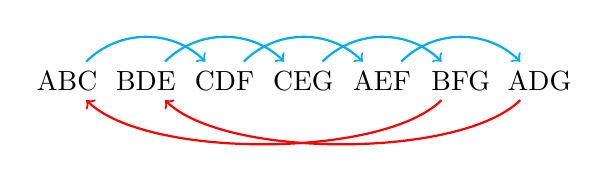
\begin{tikzpicture}
    \node(1) {ABC};
    \node[right of=1] (2) {BDE};
    \node[right of=2] (3) {CDF};
    \node[right of=3] (4) {CEG};
    \node[right of=4] (5) {AEF};
    \node[right of=5] (6) {BFG};
    \node[right of=6] (7) {ADG};
    \draw[->, thick]
    (1) edge[cyan, out=45, in=135, looseness=1,] (3)
    (2) edge[cyan, out=45, in=135, looseness=1,] (4)
    (3) edge[cyan, out=45, in=135, looseness=1,] (5)
    (4) edge[cyan, out=45, in=135, looseness=1,] (6)
    (5) edge[cyan, out=45, in=135, looseness=1,] (7)
    (6) edge[red, out=-135, in=-45, looseness=0.6,] (1)
    (7) edge[red, out=-135, in=-45, looseness=0.6,] (2)
;

\end{tikzpicture}
    \caption{Material transpositions}
    \label{fig:polillas-material-transposition}
\end{figure}

So for a transposition of ABC$\rightarrow$CDF: A maps to C, B maps to D, and C maps to F. In this way, the sequence of events produced by the transposition process is slightly unpredictable as materials do not map directly on to one another. At the beginning of the second sequence, A is mapped to C, but later in that same sequence A maps onto itself.

\begin{table}[H]
    \centering
\resizebox{\columnwidth}{!}{
\begin{tabular}{ c | c c c c c | c c c | c c c c c c | c c c | c c c | c c | c c c }
sections & [01] &  &  &  &  & [02] &  &  & [03] &  & & & & & [04] & & & [05] & & & [06] & & [07] & & \\  
  moments & \textcolor{red}{1}&\textcolor{red}{2} &\textcolor{red}{3} &\textcolor{red}{4} &\textcolor{red}{5} &\textcolor{red}{6} &\textcolor{red}{7} &\textcolor{red}{8} &\textcolor{red}{9} &\textcolor{red}{10} &\textcolor{red}{11} &\textcolor{red}{12} &\textcolor{red}{13} &\textcolor{red}{14} &\textcolor{red}{15} &\textcolor{red}{16} &\textcolor{red}{17} &\textcolor{red}{18} &\textcolor{red}{19} &\textcolor{red}{20} &\textcolor{red}{21}  &\textcolor{red}{22} &\textcolor{red}{23} &\textcolor{red}{24} &\textcolor{red}{25} \\  
  \midrule
  materials & & & & \colorbox{white}{A} & & & & B & & & & & C & E & & \colorbox{white}{A} & & & & & B & A & & &  \\  
 & A & A & B & B & B & D & E & E & C & D & C & C & E & \colorbox{white}{G} & \colorbox{white}{A} & E & E & B & F & F & G & \colorbox{white}{D} & \colorbox{white}{D} & \colorbox{white}{D} & G \\ 
 & & & C & C & & & & & \colorbox{white}{F} & & & & & & F & F & & & & & & G & G & &  \\  
\end{tabular}
}
\caption{Polillas moments part 1}
    \label{fig:p-moments-1}
\end{table}

\begin{table}[H]
    \centering
\resizebox{\columnwidth}{!}{
\begin{tabular}{ c | c c | c c | c c c | c c c | c c c | c c c c | c c | c c | c c c c }
sections & [08] &  & [09] &  & [10] &  &  & [11] &  &  & [12] & & & [13] & & & & [14] & & [15] & & [16] & & & \\  
  moments & \textcolor{red}{26}&\textcolor{red}{27} &\textcolor{red}{28} &\textcolor{red}{29} &\textcolor{red}{30} &\textcolor{red}{31} &\textcolor{red}{32} &\textcolor{red}{33} &\textcolor{red}{34} &\textcolor{red}{35} &\textcolor{red}{36} &\textcolor{red}{37} &\textcolor{red}{38} &\textcolor{red}{39} &\textcolor{red}{40} &\textcolor{red}{41} &\textcolor{red}{42} &\textcolor{red}{43} &\textcolor{red}{44} &\textcolor{red}{45} &\textcolor{red}{46}  &\textcolor{red}{47} &\textcolor{red}{48} &\textcolor{red}{49} &\textcolor{red}{50} \\  
  \midrule
  materials & & & & \colorbox{cyan}{C} & & & & C & & & & & B & F & & \colorbox{yellow}{A} & & & & & A & B & & &  \\  
 & C & C & D & D & C & E & G & G & A & E & B & B & F & \colorbox{yellow}{G} & \colorbox{yellow}{A} & D & D & A & B & B & C & \colorbox{yellow}{D} & \colorbox{yellow}{D} & \colorbox{yellow}{D} & E \\ 
 & & & F & F & & & & & \colorbox{yellow}{F} & & & & & & G & G & & & & & & E & E & &  \\  
\end{tabular}
}
\caption{Polillas moments part 2}
    \label{fig:p-moments-2}
\end{table}

\begin{table}[H]
    \centering
\resizebox{\columnwidth}{!}{
\begin{tabular}{ c | c c c c | c c c c c | c c c | c c c c c | c c c c | c c c c }
sections & [17] &  &  &  & [18] &  &  &  &  & [19] & & & [20] & & & & & [21] & & & & [22] & & & \\  
  moments & \textcolor{red}{51}&\textcolor{red}{52} &\textcolor{red}{53} &\textcolor{red}{54} &\textcolor{red}{55} &\textcolor{red}{56} &\textcolor{red}{57} &\textcolor{red}{58} &\textcolor{red}{59} &\textcolor{red}{60} &\textcolor{red}{61} &\textcolor{red}{62} &\textcolor{red}{63} &\textcolor{red}{64} &\textcolor{red}{65} &\textcolor{red}{66} &\textcolor{red}{67} &\textcolor{red}{68} &\textcolor{red}{69} &\textcolor{red}{70} &\textcolor{red}{71}  &\textcolor{red}{72} &\textcolor{red}{73} &\textcolor{red}{74} &\textcolor{red}{75} \\  
  \midrule
  materials & & & & \colorbox{pink}{A} & & & & \colorbox{pink}{B} & & & & & A & B & & B & & & & & \colorbox{cyan}{C} & C & & &  \\  
 & \colorbox{pink}{A} & \colorbox{pink}{A} & E & E & \colorbox{pink}{B} & F & \colorbox{yellow}{G} & \colorbox{yellow}{G} & \colorbox{yellow}{A} & \colorbox{pink}{D} & A & A & \colorbox{cyan}{B} & C & B & \colorbox{yellow}{D} & \colorbox{yellow}{D} & C & D & D & F & \colorbox{cyan}{E} & \colorbox{cyan}{E} & E & \colorbox{pink}{G} \\ 
 & & & \colorbox{yellow}{F} & \colorbox{yellow}{F} & & & & & G & & & & & & E & \colorbox{orange}{E} & & & & & & \colorbox{pink}{G} & \colorbox{pink}{G} & &  \\  
\end{tabular}
}
\caption{Polillas moments part 3}
    \label{fig:p-moments-3}
\end{table}

In the figures above, yellow highlights refer to materials in the same position as the preceding transposition. Blue highlights refer to materials in the same point in time but not the same vertical position as the preceding transposition. Pink highlights refer to materials in the same position as the original transposition. Red highlights refer to materials in the same point in time but not the same vertical position as the original transposition.

\subsection{Material A}

Material \boxed{\text{A}} consists primarily of gestured derived from glissando motions. I sketched seven available manifestations of the material, not all of which occur in the final work. The narrative arc of this material was meant to be the gradual revelation of higher partials of the fundamental provided by open strings across the ensemble. The open strings were chosen so that no instrument would have octavations of the same harmonic series. I also wanted to avoid a common trope which occurs when many natural harmonics are used in a work. It can be difficult to avoid the impression of the stack of perfect fifths representing the tuning of the strings of each instrument. By retuning the cello's \textit{IV} string from C\mynatural \hspace{0.12cm}to a lower B\myflat, I was able to create a whole-tone chord voiced entirely with open strings. Several other materials feature a significant manifestation where the glissando motion has infected the pre-established nature of the material. This is never the product of a \textit{ligature} material juxtaposition, as if material \boxed{\text{A}} and another material were listed as being performed simultaneously in the form diagram, rather the glissandi represent a doppelgänger effect of convergent evolution.

\begin{enumerate}
\item damped glissando
\item damped trills with shallow gliss
\item natural harmonic gliss (B\myflat1 C\mynatural3 D\mynatural4 E\mynatural5)
\item sustain + unidirectional gliss (intentionally rhythmic) slow$\rightarrow$fast, norm$\rightarrow$circular bow, 
\item \textcolor{red}{x} bow contact points + gliss: same bowing + different rhythm OR same rhythm + different bowing
\item glissando tremolo — shallow gliss: change string contact point, change tremolo speed, talea with intermittent short durations to anchor tremolo
\item flautando full bows
\end{enumerate}

\subsection{Material B}

Material \boxed{\text{B}} develops in two different directions. One aspect of \boxed{\text{B}} is the harmonic language and the other is the bowing technique used at the opening of the work. One developmental trajectory is the gradual slowing of individual spazzolato articulations, developing from swipes of barely audible pitch to perforated sounds of crunching bow hair. The other is the gradual crystallization of rigorous harmonic manipulations, almost always formalized as ratios above a fundamental even when notated as quarter tones. These trajectories result in two culminations from measures 188-210 and 258-273 respectively.

\begin{enumerate}
\item talea — repeat pitches by group
\item sputtering — potamia
\item grand interpolation (scratch$\rightarrow$normale$\rightarrow$slow bow$\rightarrow$\ac{XSB}) — voice-led from previous
\item chorale — Just Intonation Tonnetz voice-led by hand
\end{enumerate}

\subsection{Material C}\label{material-C-summary}

\boxed{\text{C}} is a mostly static material. The pitch process in these materials is usually static with occasional voice-leading. The rhythmic language is polyrhythmic. Each voice is given a different prolation value and talea of a long value followed by a short value. The short value is used to accent the polyrhythm as an anchor point for an articulation such as an accent, tremolo, or circular bowing.

\begin{enumerate}
\item sustain with intermittent accent, tremolo, gliss
\item tremolo$\rightarrow$circular bowing$\rightarrow$normale
\item tremolo with \lilyTimeSignature{1}{6} metric interruption circular bowings
\item \textcolor{red}{x} cascading spatial notation
\end{enumerate}

\subsection{Material D}

Material \boxed{\text{D}} is represented by various trills. The trills are mostly used as a method whereby the duration of each measure is clearly heard. The trill gestures are almost always proportionally related directly to the measure duration. The pitch material is derived from traditional serial pitch manipulation but eventually develops as a sliding glissando figure in contrary motion.

\begin{enumerate}
\item unision attacks
\item cascades
\item duets
\item \textcolor{red}{x} grace-note anticipations
\end{enumerate}

\subsection{Material E}

\boxed{\text{E}} is similar to \textit{Akasha}'s microtonal polyphony material. The main identifying feature of \boxed{\text{E}} is the use of explicitly notated bow speeds in the form of bow contact point fractions. This produces incredibly unique and unevenly distributed bowing colors of varying degrees of scratch and flautando. The harmony features stepwise motion in quarter-tonal pitch space. Occasionally these stepwise quarter tones are derived from voicings of the harmonic spectrum. Local dynamic trajectories are also a key element.

\begin{enumerate}
\item frozen + grand interpolation / suddenly removed: accumulate divisions $\frac{7}{8}, \frac{1}{8}, \frac{9}{8}, \frac{2}{8}$ talea
\item growth or ``manifest'': gradually accelerate
\item revisit stage 1 with explicit bow contact points: \ac{XSB}$\rightarrow$slow bow$\rightarrow$ordinario$\rightarrow$flautando
\item reverse stage 2
\end{enumerate}

\subsection{Material F}

\boxed{\text{F}} is characterized as the staccato material. Sometimes taking the form of gettati and sometimes taking the form of tight, violent attacks, the general harmonic trajectory is infinite ascension of the same repeating motif. Variation is produced by the rhythmic material and type of attack used to produce each sound. 

\begin{enumerate}
\item clock ticks
\item hocketted, voice-led, stepwise melody
\item gettato that sometimes goes behind the bridge
\item grand interpolation, ascending like \textit{Akasha}, dense$\rightarrow$sparse
\item gettati$\rightarrow$multi-staccati
\item feather-beam gettato repeat x6
\end{enumerate}

\subsection{Material G}

Finally material \boxed{\text{G}} is mostly performed by bowing directly on the wood of the bridge. Occasionally, the bow drifts away from the wood in either direction, once leading to bowing behind the bridge, and ending the piece bright, shimmering overtones. The rhythmic material is usually a very simple, repeating talea, but occasionally is produced by an accumulation of attack density with an even-division rhythm maker.

\begin{enumerate}
\item shrieks, bowed on wrapping, sparse$\rightarrow$dense
\item white noise, \lilyDynamics{ppp}, occasional tremolo
\item revisit stage 2 + \ac{CLT}
\item revisit stage 2 + occasional gettato
\item revisit stage 1 + dense$\rightarrow$sparse
\item bow on the body of the instrument
\end{enumerate}

\begin{figure}[p]
    \centering
    \rotatebox{90}{
    \resizebox{!}{\textwidth}{
\begin{tikzpicture}[
node distance = 25mm and 15mm,
every edge quotes/.style = {font=\footnotesize, rectangle, draw, fill=white}
                    ]
    \node(1) {$40$};
    \node[right of=1] (2) {$60$};
    \node[right of=2] (3) {$66 \frac{2}{3}$};
    \node[right of=3] (4) {{72}};
    \node[right of=4] (5) {{90}};
    \node[right of=5] (6) {{120}};
    \node[right of=6] (7) {{130}};
    \draw[->, thick]
    (1) edge[red, out=45, in=135, looseness=2, "4:13"] (7)
    
    (1) edge[red, out=45, in=135, looseness=2, "1:3"] (6)
    (2) edge[red, out=45, in=135, looseness=2, "6:13"] (7)

    (1) edge[red, out=45, in=135, looseness=2, "4:9"] (5)
    (2) edge[red, out=45, in=135, looseness=2, "1:2"] (6)
    (3) edge[red, out=45, in=135, looseness=2, "20:39"] (7)

    (1) edge[red, out=45, in=135, looseness=2, "5:9"] (4)
    (2) edge[red, out=45, in=135, looseness=2, "2:3"] (5)
    (3) edge[red, out=45, in=135, looseness=2, "5:9"] (6)
    (4) edge[red, out=45, in=135, looseness=2, "36:65"] (7)

    (1) edge[red, out=45, in=135, looseness=2, "3:5"] (3)
    (2) edge[red, out=45, in=135, looseness=2, "5:6"] (4)
    (3) edge[red, out=45, in=135, looseness=2, "20:27"] (5)
    (4) edge[red, out=45, in=135, looseness=2, "3:5"] (6)
    (5) edge[red, out=45, in=135, looseness=2, "9:13"] (7)

    (1) edge[red, out=45, in=135, looseness=2, "2:3"] (2)
    (2) edge[red, out=45, in=135, looseness=2, "9:10"] (3)
    (3) edge[red, out=45, in=135, looseness=2, "25:27"] (4)
    (4) edge[red, out=45, in=135, looseness=2, "4:5"] (5)
    (5) edge[red, out=45, in=135, looseness=2, "3:4"] (6)
    (6) edge[red, out=45, in=135, looseness=2, "12:13"] (7);

    \draw[<-, thick]
    (1) edge[cyan, out=-45, in=-135, looseness=2, "13:4"] (7)
    
    (1) edge[cyan, out=-45, in=-135, looseness=2, "3:1"] (6)
    (2) edge[cyan, out=-45, in=-135, looseness=2, "13:6"] (7)

    (1) edge[cyan, out=-45, in=-135, looseness=2, "9:4"] (5)
    (2) edge[cyan, out=-45, in=-135, looseness=2, "2:1"] (6)
    (3) edge[cyan, out=-45, in=-135, looseness=2, "39:20"] (7)

    (1) edge[cyan, out=-45, in=-135, looseness=2, "9:5"] (4)
    (2) edge[cyan, out=-45, in=-135, looseness=2, "3:2"] (5)
    (3) edge[cyan, out=-45, in=-135, looseness=2, "9:5"] (6)
    (4) edge[cyan, out=-45, in=-135, looseness=2, "65:36"] (7)

    (1) edge[cyan, out=-45, in=-135, looseness=2, "5:3"] (3)
    (2) edge[cyan, out=-45, in=-135, looseness=2, "6:5"] (4)
    (3) edge[cyan, out=-45, in=-135, looseness=2, "27:20"] (5)
    (4) edge[cyan, out=-45, in=-135, looseness=2, "5:3"] (6)
    (5) edge[cyan, out=-45, in=-135, looseness=2, "13:9"] (7)

    (1) edge[cyan, out=-45, in=-135, looseness=2, "3:2"] (2)
    (2) edge[cyan, out=-45, in=-135, looseness=2, "10:9"] (3)
    (3) edge[cyan, out=-45, in=-135, looseness=2, "27:25"] (4)
    (4) edge[cyan, out=-45, in=-135, looseness=2, "5:4"] (5)
    (5) edge[cyan, out=-45, in=-135, looseness=2, "4:3"] (6)
    (6) edge[cyan, out=-45, in=-135, looseness=2, "13:12"] (7)
    ;

\end{tikzpicture}
}
}
    \caption{Tempo Map}
    \label{fig:apolillas-tempo}
\end{figure}

\begin{figure}[p]
\centering
    \rotatebox{90}{
    \resizebox{!}{0.9\textwidth}{
    \includegraphics[width=6in,page=1]{lilypond/polillas_graph.pdf}
}
}
    \caption{Page 1 of the color-coded graph of the large-scale form of Polillas}
    \label{fig:Polillas-graph-1}
\end{figure}

\begin{figure}[p]
\centering
    \rotatebox{90}{
    \resizebox{!}{0.9\textwidth}{
    \includegraphics[width=6in,page=2]{lilypond/polillas_graph.pdf}
    }
    }
    \caption{Page 2 of the color-coded graph of the large-scale form of Polillas}
    \label{fig:Polillas-graph-2}
\end{figure}

\subsection{Tempo}

A technique I derived from Bača's composition \textit{(HARMONY)}, for narrator and nine players, was the formulation of a reservoir of tempi. These tempi originated from a specific sequence of metric modulations. I produced a graph of all of the ratio relationships between each tempo in order to be able to modulate from one speed to any other in the reservoir. In actual practice, these modulations are not foreshadowed by an anchoring rhythm which crosses the boundary of the modulation, rather they are abrupt changes of speed. See figure \ref{fig:apolillas-tempo}.

Another possible embedding of this map is as a complete graph as seen in figure \ref{fig:polillas-tempo-2}. The only tempo which exists outside of the standard modulatory system is 108. I decided that this tempo was to be considered a ``dead end.'' The only way to modulate to or from 108 is through 90.

\begin{figure}
    \centering
\begin{tikzpicture}
  \graph[clique, n=7, clockwise, radius=2cm]
  {
    1/"$40$", 2/"$60$", 3/"$66\frac{2}{3}$", 4/"$72$", 5/"$90$", 6/"$120$", 7/"$130$"
  };
  \node[left of=5] (8) {$108$};
  \draw[<->]
  (5) edge[red, out=180, in=0, looseness=2, "$6:5$"] (8);
\end{tikzpicture}
    \caption{Alternate embedding of Tempo relationships as a complete graph}
    \label{fig:polillas-tempo-2}
\end{figure}

\section{Interpretation of Outline}

The interpretation of the three-layered outline was totally free. Generally the central line was to be considered as the foreground and the upper and lower lines were to be considered background counterpoint. At each moment, I decided what type of relationship concurrent materials should share.

While it is unlikely that the piece can be audibly interpreted as a binary, the second page of the color-coded graph reveals more oppositional relationships. I wanted the music after the large chorale section to somehow disintegrate due to its own futility. Materials are always interrupted and don't see culmination until the emergence of traditional beauty at the end of the work, drawn out of the originally toneless bridge material, only to be pull away: denying resolution in the final breath of the piece. By defining the materials and their developmental trajectories in the abstract, I was able to specify and implement various developments and transitions and to structurally distribute them where I believed they would be most effective.

\section{Conclusion}

In Polillas, I developed my own version of a combination of processes developed by Francisco Guerrero and Trevor Bača. As a user of the Abjad \ac{API} for \ac{FSC}, I inherit more explicitly from works like \textit{Akasha}. However, much of the same types of formalizations and combinatorial practices exist within my compositions as well. These techniques were further developed in my sinfonietta \textit{Alu} by way of the expanded capabilities for counterpoint in the large, diverse ensemble setting.\footnote{The complete source code for \textit{Polillas} can be found at \url{https://github.com/GregoryREvans/polillas}} 
\begin{savequote}[75mm]
The technique of combinatorics made it possible to establish relationships, which could go from the first flute to the last double bass: very tense connections throughout the work, nothing evident to the ear or the eye, but important to maintain the structural fact. [...] At a macroscopic level it was possible for us to see the whole work from afar and give an explanation of the \emph{why} of a particular note, although the composer could vary something he did not like.
\qauthor{Francisco Guerrero Marín\footnote{\citet[175]{guerrero-quote}}}
\end{savequote}

\chapter{\textit{Alu} (2024) for Sinfonietta}
\label{Chapter4}
% \lettrine[lines=2,slope=-2pt,nindent=2pt]{\textcolor{SchoolColor}{A}}{lu, for sinfonietta,}

\lettrine[lines=3]{\setmainfont{GoudyInitialen}[Path=./fonts/, Extension = .ttf]\color{printGreen}A}{lu for sinfonietta,} just like \textit{Polillas,} was influenced directly by my study of the preceding works. The large-scale formal architecture is informed by a fusion of the approaches of Guerrero and Bača, the material definitions are more closely related to those employed by Guerrero, and the freely experimental yet structural nature of the harmonic language seen in Barraqué is the spiritual successor to the harmonic language of this work. \textit{Alu} is perhaps also in dialogue with my 2018 work for 21 saxophones given the (admittedly naïve) title \textit{GUERRERO}, representing one of my earliest acknowledged compositions.

When adapting one's compositional technique to the environment afforded by computation, there appears to be a trend toward the dissolution of motivicity, or at least rhythmic directionality: it is trivial to produce page upon page of related rhythmic materials for even a large ensemble in just a few short moments; however, wallpapering the resonant chamber of a concert hall with unending, anonymous textures is rarely compelling composition. This is not only a common pitfall for composers thrust for the first time into the potentially alienating arena of musical formalization, this was my personal struggle when I first adopted such a compositional process. My composition \textit{GUERRERO,} while remaining an official component of my œuvre, can certainly be read as a ``wallpapering'' listening experience.

As previously hinted, my works \textit{Torlannol} and \textit{Infiorescenze} portend a shift in my musical language away from the mass textures which characterize much of my music until now. It felt fitting then, here at the end of my doctoral studies, to revisit the possibilities of the swarming mass textures of \textit{GUERRERO} made particularly powerful in the context of a large ensemble such as a sinfonietta, now also making use of my newly established criteria for strong formal structures.

\section{Desiderata}

I have a tendency to title compositions with a single word, often in a language other than English. This could be read as a banal exoticism; however, the habit is the result of a twofold æsthetic pressure. I am not typically comfortable deploying titles conventionally attributed to classical genres such as ``sonata,'' ``symphony,'' or ``concerto,'' but referring to a work as ``Composition no.1 for orchestra'' as was popular for a time in the 1950's feels unremarkable. Neither am I comfortable with extramusical meaning being used to justify the musical discourse of a work and my relationship to text in music is particularly fraught. What then am I to do? It has been my practice to compromise on the subject of extramusical meaning by using a creative word or phrase as a title and writing that title in a language, or better yet a writing system, other than what is native to me, placing that extramusical meaning at a distance. There is however, an extra-musical significance to the title and the basic gestural qualities to each material.

The title of the work \textit{Alu}, a word found on many runestones, does not have a clear definition. It is thought to mean ``ale'' (i.e. alcohol) and is used to mean ``bravery,'' ``strength,'' ``protection,'' as well as many other translations. The inscription of Alu becomes an amulet over time, appearing in isolation or in an abstracted context. Runestones can be notoriously difficult to decipher. Various forms of cryptography are used in runestone carving. A famous use of cipher runes can be found on the Rökstenen carved around 800 CE. Henrik Williams, in his book ``Rökstenen och världens undergång,'' illustrates a possible interpretation of the content of the stone as well as an interpretation of the kennings and cipher runes on the stone.

In reaching for a relationship to runestones, I am not attempting to force, as has unfortunately been historically precedent, a white ethno-nationalist æsthetic. The Armanen runes invented in 1906 and various icons in Nazi symbology draw on runes to project a false pagan history rooted in Northern Europe in an attempt to distance European Christianity's relationship to Judaism and other aspects of Semitic history. While the use of runes, especially typography which features either the Elder or Younger Futhark, carries the baggage of a white ethno-nationalist connotation,\footnote{Perhaps especially so in the current political climate of the United States} my admiration for the carving of runestones lies in the subterfuge of this particular literate tradition.

Material \boxed{\text{A}} is meant to be reminiscent of the sound of chiseling and is eventually meant to be transfigured into the ticking of a clock. Material \boxed{\text{B}} is meant to illustrate a kind of entropy on the geologic time scale: earth erodes and plant life encroaches on the edifices erected by humanity. Material \boxed{\text{C}} is perhaps the sound of the growing plant life itself or the falling rain. Something in this material echoes the revving of the engine of a sports car in the distant future relative to the carving of a runestone. Material \boxed{\text{D}} was meant to be the scraping of a stone being dragged from the location of its carving to the final, permanent resting place. The rest of the materials have no explicit, literal meaning. A runestone was typically erected as a memorial to the passing of a loved one or a momentous historical occasion. Here, I erect my stone in honor of the end of a particular time in my life as a student and tell myself ``alu: be protected and have courage.''

\section{Inherited Techniques}

Many of the techniques used to compose this piece were directly inherited from the composers described earlier in this dissertation. The large-scale structure is influenced by Guerrero's use of steiner systems. The rhythmic language of the piece is influenced bu Bača's rhythm-making techniques.

\section{Formal Permutations}

In \textit{Polillas,} I derived certain formal structures from the Fano plane, leading to the decision to use seven basic materials. In \textit{Alu,} as a result of my desire to use more than seven materials, I derive structures from the Affine plane. The Affine plane is a solution to Steiner system S(2, q, q\textsuperscript{2}). The system S(2, 3, 9) features arrangements of nine elements and resolves to S=((ABC, BDI, DEF, ECG, CFI, FGB, GHI, HBE, EAI, ADG, DHC, HFA)). The plane contains n\textsuperscript{2} points, each point is contained in n+1 lines, and there are n\textsuperscript{2}+n lines.

\begin{figure}[H]
    \centering
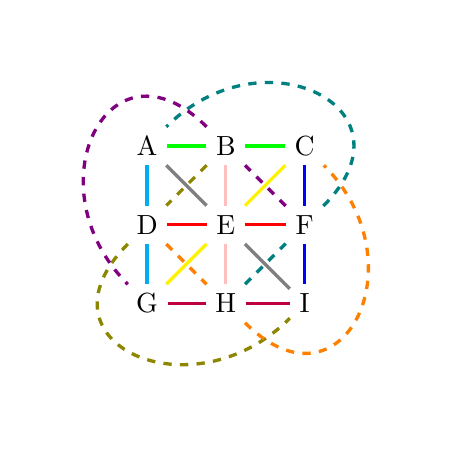
\begin{tikzpicture}
    \node(1) {A};
    \node[right of=1] (2) {B};
    \node[right of=2] (3) {C};
    \node[below of=1] (4) {D};
    \node[below of=2] (5) {E};
    \node[below of=3] (6) {F};
    \node[below of=4] (7) {G};
    \node[below of=5] (8) {H};
    \node[below of=6] (9) {I};
    \draw[-, very thick]
    (1) edge[green] (2)
    (2) edge[green] (3)
    (4) edge[red] (5)
    (5) edge[red] (6)
    (7) edge[purple] (8)
    (8) edge[purple] (9)
    (3) edge[yellow] (5)
    (5) edge[yellow] (7)
    (1) edge[gray] (5)
    (5) edge[gray] (9)
    (3) edge[blue] (6)
    (6) edge[blue] (9)
    (1) edge[cyan] (4)
    (4) edge[cyan] (7)
    (2) edge[pink] (5)
    (5) edge[pink] (8)
    (2) edge[olive, dashed] (4)
    (4) edge[olive, dashed, out=225, in=225, looseness=2] (9)
    (4) edge[orange, dashed] (8)
    (8) edge[orange, dashed, out=315, in=315, looseness=2] (3)
    (8) edge[teal, dashed] (6)
    (6) edge[teal, dashed, out=45, in=45, looseness=2] (1)
    (6) edge[violet, dashed] (2)
    (2) edge[violet, dashed, out=135, in=135, looseness=2] (7); 

\end{tikzpicture}
    \caption{Affine Plane}
    \label{fig:affine-plane}
\end{figure}

Five main material collections derive from a re-partitioning of the plane into ((ABC), (BDI, DEF), (ECG, CFI, FGB), (GHI, HBE, EAI), (ADG, DHC, HFA)). I then simplify each partition to (ABC, BDIEF, ECGFIB, GHIBEA, HFADCG). I calculate combinations from each partition from size 1-4 and select those which I feel are musically compelling to produce the sequence ((A, B, A, BC, A), (B, BD, BIE, BDEF, BF), (CF, C, CGI, CB, ECFB, C), (HB, H, HIE, HA, GHBA, H), (A, AC, HADC, G, GC, GCD, GCDA, A)). Each of the five main sequences has a primary material: sequence one primarily features \boxed{\text{A}}, two features \boxed{\text{B}}, three features \boxed{\text{C}}, four features \boxed{\text{H}}, and sequence five emphasizes \boxed{\text{A}} at the beginning and end, but emphasizes \boxed{\text{G}} in the center. Sequences three and four are arranged as ciphers of one another. They share the same structure yet expose different materials.

\subsection{Main Sections}

In composing \textit{Alu,} I wanted to take several risks by using unfamiliar composing strategies. First, the work is divided into a main binary structure, distinct from my typical narrative structures. The first section represents one long, stable glow, perhaps under the metaphorical haze of historical time. The materials are meant to freely overlap, coexisting rather than having an oppositional or teleological relationship. The second section is meant to more rigidly contrast a wide variety of materials. The materials of the second section, in contrast to the first, are meant to refuse development.

The formal design of \textit{Alu} begins with the definition of 5 proportions which are used to calculate the duration of each main section of the work. The proportions divide \textit{Alu} into an \textbf{introduction} with a proportional value of $1$, \textbf{section A} with a proportional value of $16 \div ϕ$, \textbf{section B} with a proportional value of $16$, and a \textbf{coda} with a proportional value of $\frac{16 \div ϕ}{ϕ}$. \textbf{Section B} subdivides into two sections to allow for the kind of structural repetition with different materials as previously seen in \textit{Polillas}, resulting in individual proportions of $8$. See figure \ref{fig:main-sections}.

\begin{figure}[p]
    \centering
    \rotatebox{90}{
    \resizebox{0.9\textheight}{!}{
\begin{tikzpicture}[
every edge quotes/.style = {font=\normalsize, rectangle, draw, fill=white}
                    ]
    \draw[pattern=crosshatch dots, pattern color=gray] (0,0) rectangle (1,1);
    \draw[pattern=crosshatch, pattern color=blue] (1,0) rectangle (11,1);
    \draw[pattern=north east lines, pattern color=orange] (11,0) rectangle (19,1);
    \draw[pattern=north west lines, pattern color=orange] (19,0) rectangle (27,1);
    \draw[pattern=crosshatch dots, pattern color=gray] (27,0) rectangle (33.25,1);

    \node (n1) at (0.5,1.25) {Intro};
    \node (n2) at (1.5,1.25) {A};
    \node (n3) at (11.5,1.25) {B1};
    \node (n4) at (19.5,1.25) {B2};
    \node (n5) at (27.5,1.25) {Coda};

    \node (n6) at (0.5,-1.25) {$1$};
    \node (n7) at (6,-1.25) {$\frac{16}{ϕ} \approx 10$};
    \node (n8) at (15,-0.25) {$8$};
    \node (n9) at (23,-0.25) {$8$};
    \node (n10) at (19,-1.25) {$8 + 8 = 16$};
    \node (n11) at (30.125,-1.25) {$\frac{16 \div ϕ}{ϕ} \approx 6.25$};

    \draw[<->, thick]
    (n7) edge[black, out=-45, in=-135, looseness=0.25, "main binary"] (n10)
    (n3) edge[black, out=45, in=135, looseness=0.25, "structural repetition"] (n4)
    ;

\end{tikzpicture}
}
}
    \caption{Basic Formal Plan}
    \label{fig:main-sections}
\end{figure}

After these proportional factors are derived, they are used to calculate the duration in seconds of each main section through the use of equation \ref{eq:guerrero-proportions}.

\begin{figure}[H]
    \centering
    1 + 10 + 8 + 8 + 6.25 = 33.25
    \caption{Proportions of main sections of \textit{Alu}}
    \label{fig:alu-props}
\end{figure}

So to perform the duration calculation on these proportions we obtain the following durations with a desired total duration of 1200'' assuming a basic tempo of \quarterNote = 60.

\begin{equation}
    D_1 = \frac{(1 \cdot 1200)}{33.25} \approx 36'' = 0.6' (\text{c.9 mm of \lilyTimeSignature{4}{4})}
\end{equation}

\begin{equation}
    D_2 = \frac{(10 \cdot 1200)}{33.25} \approx 361'' = 6' (\text{c.90 mm of \lilyTimeSignature{4}{4})}
\end{equation}

\begin{equation}
    D_3 = \frac{(8 \cdot 1200)}{33.25} \approx 289'' = 4.8' (\text{c.72 mm of \lilyTimeSignature{4}{4})}
\end{equation}

\begin{equation}
    D_4 = \frac{(8 \cdot 1200)}{33.25} \approx 289'' = 4.8' (\text{c.72 mm of \lilyTimeSignature{4}{4})}
\end{equation}

\begin{equation}
    D_5 = \frac{(6.25 \cdot 1200)}{33.25} \approx 226'' = 3.8' (\text{c.56 mm of \lilyTimeSignature{4}{4})}
\end{equation}

Each subsection of \textbf{B} is divided by the same set of proportions.

\begin{equation}
    d_1 = \frac{(1 \cdot 289)}{33.25} \approx 9'' = 0.15' (\text{c.2 mm of \lilyTimeSignature{4}{4})}
\end{equation}

\begin{equation}
    d_2 = \frac{(10 \cdot 289)}{33.25} \approx 87'' = 1.45' (\text{c.22 mm of \lilyTimeSignature{4}{4})}
\end{equation}

\begin{equation}
    d_3 = \frac{(8 \cdot 289)}{33.25} \approx 70'' = 1.167' (\text{c.17 mm of \lilyTimeSignature{4}{4})}
\end{equation}

\begin{equation}
    d_4 = \frac{(8 \cdot 289)}{33.25} \approx 70'' = 1.167' (\text{c.17 mm of \lilyTimeSignature{4}{4})}
\end{equation}

\begin{equation}
    d_5 = \frac{(6.25 \cdot 289)}{33.25} \approx 54'' = 0.9' (\text{c.13 mm of \lilyTimeSignature{4}{4})}
\end{equation}

These values are then adjusted for tempo changes resulting in:

\begin{table}[H]
    9mm at \quarterNote=$46\frac{2}{3}$ = 7mm
    
    90mm at \quarterNote=$87\frac{1}{2}$ = 131mm
    
    2mm at \quarterNote=$122\frac{1}{2}$ = 4mm
    
    22mm at \quarterNote=$105$ = 38mm
    
    18mm at \quarterNote=$87\frac{1}{2}$ = 26mm
    
    18mm at \quarterNote=$70$ = 21mm
    
    14mm at \quarterNote=$105$ = 24mm
    
    56mm at \quarterNote=$70$ = 65mm
    
    total: 429 mm
    \caption{Measure counts of subsections reproportioned by tempo}
    \label{tab:rescaled-measure-groups}
\end{table}

These measure counts are then used for each subsection regardless of whether the time signature process produces a time signature other than \lilyTimeSignature{4}{4}. The section boundaries are as follows:

\begin{table}[H]
    % \centering
    \begin{tabular}{c|l}
        Section & Measures \\
        \toprule
        1 & 1-7 \\
        2 & 8-138 \\ 
        3 & 139-142 \\ 
        4 & 143-180 \\ 
        5 & 181-206 \\ 
        6 & 207-227 \\
        7 & 228-251 \\
        8 & 252-255 \\
        9 & 256-293 \\
        10 & 294-319 \\
        11 & 320-340 \\
        12 & 341-364 \\
        13 & 365-430 \\
    \end{tabular}
    \caption{Sections in \textit{Alu}}
    \label{tab:alu-sections}
\end{table}

\section{Basic Materials in \emph{Alu} and their Available Manifestations}

The basic elements of \textit{Alu} comprises 9 materials.

% \begin{tikzpicture}
    
%     % Draw tick marks and labels
%     \foreach \x in {0,...,11} {
%         \draw (\x,0.1) -- (\x,-0.1) node[below] {\x};
%     }
% \end{tikzpicture}
% \\

% \begin{tikzpicture}
    
%     % Draw tick marks and labels
%     \foreach \x in {0,0.5,...,5.5} {
%         \draw (\x,0.1) -- (\x,-0.1) node[below] {\x};
%     }
% \end{tikzpicture}
% \\

% \begin{tikzpicture}
    
%     % Draw tick marks and labels
%     \foreach \x in {0,1.5,...,16.5} {
%         \draw (\x,0.1) -- (\x,-0.1) node[below] {\x};
%     }
% \end{tikzpicture}

\subsection{Material A}

Material \boxed{\text{A}} is dynamic, featuring three rhythmic variations. The chisel rhythms, representative of past, inaccurate methods of measuring time (or enjoying it) are unstable. These rhythms accelerate and decelerate with occasional gaps in the surface texture. The sound of wood in the percussion is also fairly un-nuanced. The future version of the material comprises rigid eighth note ticks performed across greater instrumental varieties. A greater accuracy in keeping time, here leads to a deeper sonic perspective of that measured space.

\subsection{Material B}

Material \boxed{\text{B}} provides primarily background or drone texture. The few variations of this material only serve to alter the level of perceived rhythmic activity and thus the fundamental energy of a given moment of music. Harmonically, this material is intended to come close to, but slightly miss the mark of traditional standards of harmonic beauty. These harmonies are derived from manipulations of the twelve note aggregate.

\subsection{Material C}

Material \boxed{\text{C}}, the glissandi, deploys a wide palette of energies. The glissandi can move in three directions: up, down, or up and immediately back down as a single gesture. What really provides the sense of contrast within each appearance of this material is the speed at which each glissando rises or falls as well as how shallow or steep of range of pitches being traversed sounds.

\subsection{Material D}

Material \boxed{\text{D}} is static, featuring a single variation. The staggered exchange rhythms in brass and percussion derives from a talea of basic durations. These durations are helianthated and rotated to a difference starting point for each instrument. For each participant in the rhythmic event, a cycle of durations are chosen to represent a sounding tone and the rest become rests. The cycles are chosen to be complementary across the instrumentation to produce an approximate cascade of gestures while avoiding overt periodicity.

\subsection{Material E}

Material \boxed{\text{E}} featuring several ambiguous variations, somewhat narrativizing my own development from pure textural music to figural writing. The variations are likely to be difficult to hear as having a relationship to one another without the priveledged knowledge of their provenance. In the beginning of the piece, \boxed{\text{E}} takes the form of runs of short ascending motifs on continuous sixteenth notes.\footnote{However, the sense of time is distorted through the use of prolations divorced from the metric fram of each measure.} The next appearance of this material begins with an upward run followed by a held tone with explicitly composed vibrato, coming closer to gesturality. More traditional figures later appear. These figures are deliberately coordinated in smaller instrumental groups to provide homorhythm, fill rhythm gaps, and to provide counterpoint.

\subsection{Material F}

Material \boxed{\text{F}} represents any piano solo passage. These passages make use of the same rhythmic materials featured in the figural passage of \boxed{\text{E}}.

\subsection{Material G}

Material \boxed{\text{G}} is static. The material comprises a drifting trill with homorhythmically coordinated glissandi.

\subsection{Material H}

Material \boxed{\text{H}} deliberately develops the surface rhythm technique described in chapter \vref{Chapter1}. These Guerrero-type pitch repetitions, themselves referential to Ikhoor by Xenakis, are more varied in their interlocking overlap than as they were deployed in \textit{Rhea}, inhabiting more than quarter note prolations.

\subsection{Material I}

Material \boxed{\text{I}} represents any bass clarinet solo. The two forms of this materials are a loud split-tone multiphonic and an irregularly accented trill which collaborates with a simpler surrounding trill texture.

\section{Conclusion}

The overall impression given by \textit{Alu} is the stability of the consistent reappearance of a primary material within each main section. \textit{Polillas,} featuring no consistent primary materials, is always shifting and changing which made clear developmental trajectories important in order to maintain interest. \textit{Alu} is afforded a greater patience because the identity of each featured material is more completely explored. This piece refuses much of my nuanced approach to color and expressivity, wending toward the fauve style. I am not entirely certain that some aspects of my compositional technique very successfully map from chamber music onto large ensemble music. As mentioned in chapter \ref{Chapter1}, Francisco Guerrero does not make use of many instrument-specific techniques in his music in order to have a simple approach to material definition for any given ensemble. I attempted a similar approach in 
\textit{Alu} for similar reasons; however, when next I compose for a larger ensemble of diverse instrumentation, I will need to reimagine my concept of a material, perhaps assisted by my development of figural writing.\footnote{The complete source code for \textit{Alu} can be found at \url{https://github.com/GregoryREvans/alu}} 
\begin{savequote}[75mm]
The treasure chest of the frequently thorny achievements of concert music after WWII, of musical modernism, is a wonder where time flows in impossible directions, sounds appear from instruments like magic, and musical logic is free to bewilder. [...] What's needed now, what's been missing for decades, is a musical answer to the magic realisms of the 20th- and 21st-century [...]. What is needed is an engagement with musical inheritance that finds space to accommodate beauty, difficulty, and the transfiguration of the one by the other, since that seems, inescapably, to be the world we live in.
\qauthor{Trevor Bača\footnote{\citet{harmonyscore}}}
\end{savequote}

\chapter{Conclusion}
\label{conclusion}

% \lettrine[lines=2,slope=-2pt,nindent=2pt]{\textcolor{SchoolColor}{I}}{n this dissertation}

\lettrine[lines=3]{\setmainfont{GoudyInitialen}[Path=./fonts/, Extension = .ttf]\color{printGreen}I}{n this dissertation}, I have described the compositional techniques of three composers who have significantly influenced my compositional approach and I have shown certain aspects of their compositional process which are present within my own work. Undoubtedly, as a result of my own use of the Abjad \ac{API} for \ac{FSC}, my music conforms more closely to that of Trevor Bača, however I have my own criteria for the configuration of formal structures and generative streams of information. In recent works, such as 2019's \textit{(HARMONY)}, Bača composes more frequently through the direct input of rhythm and pitch materials, leaving generative process for the proliferation of more tedious tasks, for instance the mass accumulation of grace-note figures.

My work has been influenced by works which have a strong coupling of musical parameters to create definite statements of identifiable musical material. In the future, I expect further developments in my music will occur in the areas of the development of motivic and figural materials as opposed to purely textural materials, as well as an increased interest in subtly drawing cross-relationships between different materials. A possible avenue of change will also be a greater propensity for the admixture of material. Increased ambiguity in the cross-relationships between different materials can also potentially provide an interesting complexification of the narrative arc of a piece. In fact, I have already begun experimenting with this process in my work \textit{Infiorescenze} for solo alto flute.

\begin{figure}[p]
\centering
    \rotatebox{90}{
    \resizebox{0.9\textheight}{!}{
    \includegraphics[width=6in]{lilypond/infiorescenze_example.pdf}
    }
    }
    \caption{A page from Infiorescenze for solo alto flute}
    \label{fig:infiorescenze}
\end{figure}

I am also increasingly interested in providing extra-musical connections to the materials within my work. This can provide a fresh, new perspective on the underlying structure of a material. Hèctor Parra's string quartet \textit{Arachne} features a material reminiscent of a spider extruding and plucking a web. This material is not treated narratively in the sense of a tone-poem, rather the figure is deconstructed and developed motivically.\footnote{This example was explained to me by the composer during the 2023 MIXTUR Festival workshops in Barcelona, Spain.} I see great potential in the development of figural materials which can be manipulated multi-parametrically as opposed to the sometimes undifferentiated quality of texture generated through Bača's rhythm makers which have become so foundational to my own rhythmic approach.

Through the process of understanding the large-scale formal qualities of the works described in this dissertation, I have begun to taxonomize my experience of these events. I detect certain effects as being provided by specific types of transition techniques. Different types of repetition\footnote{Here I mean literal, immediate repetition by way of repeat bar lines rather than long-term recurrence relationships throughout the course of a work.} have different psychological effects in the memory timestream of my listening experience. While I am certain my experience of these formal moves and others which I have not mentioned are entirely subjective, I am encouraged to continue taxonomizing these event-types in order to help guide my future compositions.

\section{Artist's Statement}

The intersection of narrativity and abstract structuralism is where my creative efforts are focused. My imagination is sparked by a combined interest in linguistic structure, writing systems and their calligraphy, and alternative methods of expression, for example the cultures of the esoteric which can be seen in the texts of alchemy and magic. I believe in the power of newness, that objects once found repulsive can become beautiful and that old thoughts can be recontextualized and thus recuperated. I believe in the power of the act of decipherment, that hidden meaning, once decoded is somehow amplified above that which is plainly said. The shared experience of taking apart an encrypted work can bring a community into being through the collaborative effort of shared discovery.

I am interested in musical form as the direct activation of the experience of memory. My sense of formal technique is inspired by the filmic experience of time-cuts, flashes forward and back in time, the dilation of time resultant from differing velocities. I view composition as the act of giving life to sound as pleasurable intensity through impossible timelines, fantastic colors, and unusual shapes. Regions of stability and directed moments of the manifestation of newness exchange with one another, sometimes in rapid succession to illicit the impression of changes of scene in the state of an infinite “meanwhile.”

I am aware of many layers of transmutation in operation at once. My works are often the result of a period of intense formalization of large-scale structures and gestural patterns. A coded language of physical possibilities is converted into the symbolic language of music notation. This notation is then interpreted by performers as a series of actions latent with meaning which is later deployed in real-time with all the accidents and imperfections inherent in this practice before an audience who are tasked with the absorption and psycho-embodiment of the sounding experience.

Preparing the score carries the same value of intensity and emotional urgency as the process of imagining the intangible sound physicalities which appear during a composition. Creating the score is a symbolic act, the product of which may only suggest a series of potential meanings, however interpretations at all levels, analytic, emotional, or otherwise have the power, when in combination with one another, to grip, concentrate, and lead the audience to a transfiguration of the secret language of symbols. The shared public experience of music should bear the intensity of the knowing and the feeling of the things of our world.

In recent compositions, I begin at the large-scale and proceed by crafting finer and finer detail. I create a story in speeds, the map of tempi which will lead the work. I study the instrumental forces involved and partition out manners of sound production, grouping together similar sound palettes and contrasting accompaniments. From these potential sound qualities, I distill patterns of motion, operations of harmonic elaboration, rhythmic qualities, dynamic trajectories, and other factors of each narratively differentiated material type. The materials are then developed. How can a sound become another sound? How can one material type be made into the doppelgänger of another? I determine the approximate duration of the work and divide the totality into subsections and metrically divide the subsections by a pattern of time signatures. I produce a timeline graph of the exchange of materials, whether they overlap or abut, in which measures they occur. Then begins the task of specifying the details in score notation.
\appendixpart{Appendices}
\begin{appendices}
    \renewcommand{\thechapter}{\setmainfont{EB Garamond}\textbf{\Greeklowalpha{chapter}}}
    \fancyhead[CO]{APPENDIX \thechapter: \leftmark}

\chapter{The Seven-Term System of Francisco Guerrero and Complete Formalization}
\label{AppendixA}

\lettrine[lines=2,slope=-2pt,nindent=2pt]{\textcolor{SchoolColor}{I}}{n the following appendix} is a translation of an article written by Francisco Guerrero Marín in collaboration with mathematician Juan José Morales in Scherzo magazine in 1990.\footnote{\citet{guerrerotopology}} This article introduces both Guerrero's 7-term system, used in the works \textit{Zayin II}, \textit{Rhea}, and \textit{Nur,} as well as his concept of topoligical invariance in formal structures. This very brief summary does not actually analyze any specific works to show the techniques in action, rather the article merely formalizes the two techniques. The topological principle seems to relate to invariant structures across sections such as rhythmic materials, numbers of silences, harmonic materials, and structural elements such as the orchestrational distribution of materials. The mathematical expression in the article is not sufficiently explained but likely refers to the proportional distribution of events, not only in the large scale form, but also within each instrumental line of a given section. Possibly, a first set of reference durations of large sections and subsections is first produced with the Equation \vref{eq:guerrero-proportions}. After this, the proportions of each voice are derived from the proportions of a different voice with the inclusion of some random variation.\footnote{Translator's note: As a result of the use of random values and cross-relationships between voices, it is impossible to reverse-engineer the process of a specific composition without a sketch archive.} In this way, each individual line of the score is in slightly longer or shorter proportion to the others, causing most section transitions to occur over an interpolation period instead of an immediate section change across the whole ensemble as is found in the older pieces, such as \textit{Zayin I}. Due to the low quality of my digital copy of the document, some small characters in the equations are difficult to discern. As a result, it has been sometimes necessary to guess their meaning.\footnote{A digital, full copy of the original magazine issue is freely available from \url{https://scherzo.es/hemeroteca/marzo-1990/}.}

\section{From `Musica Y Tecnologia' of issue 43 of \textit{Scherzo}}

\textbf{Music and Topology}

Zayin II, for string trio, Rhea, for twelve saxophones, and above all Nur, for choir, have been the starting points when establishing a part of the theoretical body that is described later. Part of it was already founded at the time of the composition of both works and the rest was deduced, expanded and inspired by the works themselves. Certain behavioral systems have been codified in order to give them a logical structure that allows their application and development. Since music is a phenomenon of expansion in time, it was thought that topology (expansion in space) could teach us behaviors of mobilities and transformations from a point of view that included partial topologies (for example fractals, chaos) and balance mechanisms that are related to information theories.

\textbf{Brief analysis of Nur}

Let S be the entire work. An element of S is each of the well-defined materials or sound events that compose it, and each of the parts of the work is class-L. Now let the following axioms be:

Axiom 1: If A and B are distinct elements of S, there exists at least one L-class containing A and B.

Axiom 2: If A and B are two distinct elements of S, there is only one L-class that contains A and B.

Axiom 3: Any two L-classes have at least one element of S in common.

Axiom 4: The L-classes are formed by three elements of S.

Thus, for example, for the set S = (A, B, C, D) there is no possibility of applying the axioms without obtaining contradictions.

For the set S = (A, B, C, D, E, F, G) we would obtain the following set of L-classes.

S= (ABC, BDE, DCF, CEG, EFA, FGB, GAD)

In this way, the content of the material of each part of the work is achieved and also defines the general form. The evolution of the material is done attending to a certain types of invariances that develop in a spatiotemporal dimension; space and time are two dimensions to which the same treatment is applied here. These invariances refer, for example, to the conservation of the number of beats (it is the minimum unit of time used: 16th note, 32nd note, etc.), to the maintenance of certain rules of constant proportion, etc., thus achieving an unstable balance that allows for evolution.

If the previous axioms defined the form and related materials, the rules that govern the proportions, both at a general level and instrumental part by part, are given by the following expression:

\begin{equation}
t(A_{i}) = \frac{T}{\displaystyle\sum_{i=1}^{n} m \Delta_{i} \textstyle\sum_{\substack{j=p\\ j \neq i}}^{p+k} t'(A_{j})} t'(A_{i})
\label{eq:rhea}
\end{equation}

Where:

T: Actual duration of the work.

t(A\textsubscript{i}): Duration of section A\textsubscript{i}.

m: Random number.

$\Delta_{i}$: Proportion parameter, dependent on section i.

$t'(A_{i})=m\Delta_{i}\displaystyle\sum_{\substack{j=p\\ j \neq i}}^{p+k} t'(A_{j})$: Time of imaginary distribution.

In this way all the elements are related and the desired formal unity is achieved.

The temporal dimension entails a notion of distance so we will have in reality a metric structure that induces a topology, being able to define other distances than the usual one, thus obtaining different metric topologies. Suppose we have two fragments of the work, $X$ and $Y$ with their corresponding topologies and we will call points of the spaces $X$ and $Y$ infinitesimal musical gestures, that is to say, they develop in a sufficiently small temporal interval (sextuplet 16\textsuperscript{th} note, 64\textsuperscript{th} note, etc.). We can define a function $f$ that takes us points of $X$ to points of $Y$. Such a function is said to be continuous if the points near point $p$ are sent by $f$ to points near $f(p)$ for any point $p$.

Two sections X and Y are said to be homeomorphic or topologically equivalent if there exists a function (one to one correspondence in this case) that sends points of X to points of Y that is continuous and such that the inverse function (the one that takes points from Y to points from X) is also continuous.

% \begin{figure}[H]
%     \centering
%     \includegraphics[width=80mm]{lilypond/graph.png}
%     %\caption{Caption}
%     \label{fig:guerrero-graph}
% \end{figure}

\begin{figure}[H]
\centering
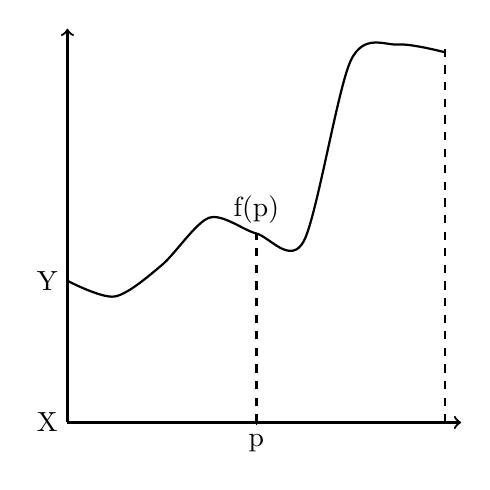
\begin{tikzpicture}
\draw[thick,->] (0,0) -- (5,0) ;
\draw[thick,->] (0,0) -- (0,5) ;
\draw (2.4 cm,1pt) -- (2.4 cm,-1pt) node[anchor=north] {p};
\draw[thick,dashed] (2.4,0) -- (2.4,2.4) node[anchor=south] {f(p)};
\draw[thick,dashed] (4.8,0) -- (4.8,4.8);
\draw [thick] plot [smooth] coordinates {(0,1.8) (0.6,1.6) (1.2,2) (1.8,2.6) (2.4,2.4) (3,2.3) (3.6,4.6) (4.2,4.8) (4.8,4.7)};
\draw (0,1.8) node[anchor=east] {Y};
\draw (0,0) node[anchor=east] {X};
% \foreach \y in {0,1,2,3,4}
%     \draw (1pt,\y cm) -- (-1pt,\y cm) node[anchor=east] {$\y$};
\end{tikzpicture}
    \label{fig:guerrero-graph}
\end{figure}

For example, the vertical projection between the straight line X and the curved line Y is a homeomorphism that intuitively is nothing more than a continuous deformation.

These continuous applications can be used to construct variations of material, since this, when evolving, creates surfaces topologically equivalent to n-toros in two dimensions where n would indicate, for example, the content in silences (the number of holes on the surface), a transformation specific to the material (unisons or its opposite, gliss, etc...).

In addition to these purely sonorous ones, others can be built whose presence is not perceptible, but which in some way direct the musical events. They are related to the abstract content of the work. This is where the use of metrics not related to temporal perception and even topological ones defined without using the notion of distance is most useful. If we define a distance we construct sets formed by elements whose distance to a given one is strictly less than a certain value. The union of all these sets (called open) determines a basis for the topological space.

Without using the notion of distance, a topological space can also be defined. Thus, given a non-empty set $X$ and for each point $p$ of $X$ a non-empty family $B(p)$ of subsets of $X$, it would be said that each family $B(p)$ is a base of open environments of point $p$ if the following properties are verified.

$B_{1}$: If $U$ is an element of $B(p)$ then $p \in U$.\footnote{TN: p is an element of U.}

$B_{2}$: If $U \in$ $B(p)$ and $V \in B(p)$ then there exists $W \in B(p)$ such that $W \not\subset U \cap V$.\footnote{TN: W is not a subset of the intersection of U and V.}

$B_{3}$: If $U \in B(p)$, for each point $q \in U$ there exists a set $V \in B(q)$ such that $V \subset U$.\footnote{TN: V is a subset of U.}

A subset $A$ of $X$ is said to be an open set when in the empty set, or when for each point $t \in A$\footnote{TN: t in A} there is a subset $U \in B(t)$ that is contained in $A$.

It is called the topology $T$ of the set $X,$ determined for the bases of open environments $B(p)$, to the family of open sets of $X$ defined by means of the bases of open environments $B(p)$.

A topological space is compact if each sequence of points has a limit point that belongs to said space. It is connected if it is made of a single piece, that is, if there are no two disjoint open spaces distinct from the vacuum, $V$ and $W$, such that $X=V \cup W$.\footnote{TN: X is the union of V and W}

It is separable (in the sense of Hausdorff)\footnote{TN: Referring to topological separation axioms.} if for every pair of points $p$ and $q$ there exist two disjoint open sets containing $p$ and $q$ respectively. Homeomorphisms preserve all topological properties such as compactness, connectedness, and separability.

Thus, then, we could build a base of open environments from whose expression the general form of the work would result and in such a way that the homeomorphisms between subspaces, whose topology was defined by such base, would control the evolution of local events; They would create rules that as such are constructed to be violated at the moment when an aesthetic choice requires it. In this way, modes of behavior can be created that encompass other destinations (molecular movements, fractalized melodic designs, etc...) but rather replace them and that in no way imply any moral direction. All of this refers to a basis of thought and not to a simple composition setting, thus resulting in empty structures that the musician must fill. It is about seeking order and not a particular order.

\phantom{text} \hfill Juan José Morales and Francisco Guerrero%\footnote{\citet{guerrerotopology}}

\section{Explanation of the Mathematical Expression}

While not every element in equation \ref{eq:rhea} is named and demonstrated, some aspects can be explained. To renotate with some simplifications, the expression could be:

\begin{equation}
X = \frac{T}{S} \cdot Y
\end{equation}

Where X is the duration of a section of the work in a particular voice, T is the total duration of the work, Y is the duration of the same section in a difference voice, and S is the sum of the duration all subsequent sections in a different voice, with some random proportional variation. If all sections and sub-sections of a work are derived from another, a source section must exist. If we take, as a basis, the system described in equation \vref{eq:guerrero-proportions} and the subsequent example proportions, we can try to calculate the proportions of a new voice with the system described in the article above. We begin with a total duration of 240, with section proporitons of 1.8, 2.4, 3.3, 3.6, and 5.4, and calculated section durations of 26.18, 34.9, 48, 52.36, and 78.54. We insert these values into the simplified equation:

\begin{equation}
V_{1}s_{1} = \frac{240}{S} \cdot 26.18
\end{equation}

Where $v1s1$ is voice 1 section 1, and S is the compound summation expression

\begin{equation}
\displaystyle\sum_{i=1}^{n} m \Delta_{i} \textstyle\sum_{\substack{j=p\\ j \neq i}}^{p+k} t'(A_{j})
\end{equation}

In this expression, there is a summation inside of another summation. The lower summation can be written as

\[
[A_{j} + A_{j + 1} + ... + A_{j+k}]
\]

Where the section identified j indications a section other than i, however the authors of the article do not define k. Without an explanation of the value of k, no further calculations are possible. The outer summation can be expressed as

\[
[m \cdot d_{1} \cdot s_{2} + m \cdot d_{2} \cdot s_{3} + ... + m \cdot d_{n} \cdot s_{n+k}]
\]

Where m is a random number, d is the proportion value of section i, and s is the summation of all section durations from j to j+k.

If we take p+k to be the number of subsequent sections, it is possible to calculate all but the final section. For this example, let us imagine that the final duration in our source set is used purely for this calculation purpose and does not represent its own section. Under these conditions we can propose a summation of

\begin{equation}
V_{1}(A_{1}) = \frac{240}{\displaystyle\sum_{i=1}^{4} m \Delta_{i} \textstyle\sum_{\substack{j=2\\ j \neq i}}^{2+k} t'(A_{j})} 26.18
\end{equation}

\subsection{Nested Summations}

i=1, m=0.75, $\Delta$=1.8, and j=2. First we sum all sections in the source durations from 2 until 5. This gives

\[
34.9 + 48 + 52.36 + 78.54 = 213.8
\]

We multiply this value with the others

\[
0.25 \cdot 1.8 \cdot 213.8 = 96.2
\]

We increment i, get a new random value and start again. i=2, m=0.9, $\Delta$=2.4, and j=3.

\[
48 + 52.36 + 78.54 = 178.9
\]

We multiply this value with the others

\[
0.1 \cdot 2.4 \cdot 178.9 = 42.9
\]

We increment i, get a new random value and start again. i=3, m=1.2, $\Delta$=3.3, and j=4.

\[
52.36 + 78.54 = 130.9
\]

We multiply this value with the others

\[
0.3 \cdot 3.3 \cdot 130.9 = 129.6
\]

We increment i one last time, get a new random value and start again. i=4, m=1, $\Delta$=3.6, and j=5.

\[
78.54 + 0 = 78.54
\]

We multiply this value with the others

\[
0.07 \cdot 3.6 \cdot 78.54 = 19.8
\]

We take the sum of these values

\[
96.2 + 42.9 + 129.6 + 19.8 = 288.5
\]

% \subsection{Time of Imaginary Distribution}

% The article says to do this but I chose not to because it's confusing? The article even has a typo there so I'm not sure if I trust it?
% $34.9 + 48 + 52.36 + 78.54 = 213.8$

% $0.045 \cdot 1.8 \cdot 213.8 = 17.32$

\subsection{Final Calculation}

This completes the whole expression. So the source value of 26.18 is recalculated as

\begin{equation}
V_{1}(A_{1}) = \frac{240}{288.5} 26.18 = 21.8
\end{equation}

This process would be repeated for each main section of the work, deriving the first voice from the source values, then deriving subsequent voices from each of the newly calculated voices. This process could conceivably be applied to subsections within a section that is used to denote a statement of more than one material type, perhaps even in the same proportions as the whole work, producing a kind of self-similarity. Note that constraining the range of the random values in this calculation has a significant effect on the resultant duration. Higher random values shorten the duration to a small output value and smaller random numbers give a result closer to the source value. So, a composer could constrain the random values to incredibly small decimals if the source value is intended to be more precise or the values could have a wider range, allowing for a more orchestrationally uncoordinated progression. To reiterate, without Guerrero's sketch materials and without a more thorough explanation of the calculation process in the Scherzo article, it is not possible to know exactly how this formula is intended to be deployed. However, the results illustrated above suggest a possible approach for deriving section durations with an interpretation of the given formula. Through the use of systems like those described above, composers have the ability to generate totally interrelated structures across the duration and instrumentation of a work which is attractive from the project of musical Modernism.\footnote{However the process described above may be incorrect. The inclusion of a random value almost totally negates any usefulness of any of the other parameters. Guerrero could just as easily have multiplied a section's projected duration by any arbitrary fraction near 1 within his own tolerance of variation.}

\section{Bača's Use of Total Formalization}

Trevor Bača's compositions from 2005-2011 use more completely formalized structures than were seen in \textit{Akasha}. What \emph{can} be seen in the compositions from this period is a greater reliance on the slow exposition of material bound to a strict algorithmic pattern. The pieces are quite long, allowing for the playing-out of the strucure underlying the form and material. The segments themselves are longer than would be the norm in later works. While the logic within each work is mostly developed without interference, much effort was taken to iterate the patterns to their ultimate form, resulting in a strikingly rigorous output. The primary aesthetic is that of the phenomenological experience.

\subsection{Po\`eme r\'ecursif (2003/05)}

\begin{quote}
\singlespacing
``Inasmuch as musical form can be equated to a through-time experience of listening for moments of musical change, the formal experience of my earlier music suggests what can understood as a phenomenological, as opposed to narrative, point of departure. \textbf{Po\`eme r\'ecursif}, for sixty-four pieces of percussion, was written in 2005 and recorded by percussionist Brian Archinal in two different mixes on his album \textit{self | space}. The music provides what is an essentially unarticulated experience of form. Tempo is fixed at the beginning of the piece and thousands of attackpoints, all played on unpitched instruments left to the choice of the performer or performers, comprise the seething texture of the music: these provide no shape equivalent to the musical phrase or section. The music ends only at the end of the piece. But the music begins many times, again and again, producing a sense of unending upwelling. Because the materials in \textit{Poème récursif} expose no musical events likely to be construed at the level of narrative -- no sudden stops or starts, no reversals, no enchaining of materials in such a way as to allow for ascriptions of causality -- perception of the music leads instead to an awareness of the act of perception itself. This metaperception is what I intend in invoking the phenomenological in the description the music: recurrent moments when the mind becomes aware of the ways that the mind experiences the music’s currents as phenomena that arise, persist and depart, overlapping in the field of perception. The materials and title of the music point to the recursion that produces these effects: every attackpoint derives from the compositing of two cellular automata over a matrix of 256 columns and 64 rows. These are interpreted, respectively, as the measures and parts of the score, dimensions comparable in some respect to the massing of 100 metronomes, though in the service of a determinism of music rather than its open specification.''\footnote{\citet{baca-dissertation}}
\end{quote}

Po\`eme r\'ecursif was originally composed in 2003 and was significantly recomposed in 2005. The simpler 2003 edition will be analyzed here as a demonstration of one avenue which Bača pursued toward totally formalizing a work in a way not too dissimilar from Guerrero's motivation for interrelatedness. This piece, for 64 individual pieces of percussion, is perhaps Trevor Ba\v{c}a's most elegant composition if his least complex. In the 2003 edition, the cellular automata are quite visually apparent at a distance. See \autoref{fig:recursifpage13}.
\begin{figure}[p] % try H or h ?
    \centering
    \includegraphics[scale=0.4]{lilypond/recursif_2003_pg_13.pdf}
    \caption{Po\`eme r\'ecursif (2003) page 13}
    \label{fig:recursifpage13}
\end{figure}

The visual immediacy of the processes within in the piece is significantly reduced in the 2005 edition, largely motivated by the desire to reduce the obvious periodicity present in the first edition. More figures cross the invisible bar lines, distorting the ever present down-beats. See \autoref{fig:recursifpage8}.

\begin{figure}[p] % try H or h ?
    \centering
    \includegraphics[scale=0.4]{lilypond/recursif_2005_pg_8.pdf}
    \caption{Po\`eme r\'ecursif (2005) page 8}
    \label{fig:recursifpage8}
\end{figure}

Composed page-by-page, only one process produces the rhythmic framework of the piece. A key component to the structure of this piece is the extensive use of the binomial coefficient $\binom{n}{k} = \frac{n!}{k!(n-k)!}$. The binomial coefficient is incorporated into the larger rhythm construction process. A voice number out of 64 is chosen along with a page number out of 16 total pages. The measure at which each page begins is calculated such that \begin{equation}16 \cdot (pageNumber - 1) + 1 = startMeasureNumber\end{equation} This means that the starting measure of page 1 is calculated \begin{equation}16 \cdot 0 + 1 = 1\end{equation} page 2 is \begin{equation}16 \cdot 1 + 1 = 17\end{equation} page 3 is \begin{equation}16 \cdot 2 + 1 = 33\end{equation} etc, which allows 16 measures per page.

After this, a series of tuplet ratios is gathered for the chosen voice and page combination while iterating through the measure numbers. A total value is calculated as \begin{equation}total = 255 + voiceNumber - measureNumber\end{equation} and a count value is calculated as \begin{equation}count = voiceNumber - 1\end{equation} The count value is then recalculated to be the binomial coefficient where $n=total$ and $k=count$. The result of the binomial coefficient function is then reduced to modulo 8, then finally truncated to an integer. If the result is $\leq 0$, a rest is returned, otherwise the number of attacks equivalent to the final count value is returned.

\begin{lstlisting}[language=Python,frame=tb,caption={Po\`eme r\'ecursif rhythm function},label=lst:recursifrhythm]
def rhythm(voice_number: int, page_number: int) -> baca.RhythmCommand:
    """
    Makes rhythm for ``voice_number`` and ``page_number``.
    """
    assert page_number in range(1, 16 + 1)
    start_measure_number = 16 * (page_number - 1) + 1
    stop = start_measure_number + 16
    measure_numbers = range(start_measure_number, stop)
    tuplet_ratios = []
    for measure_number in measure_numbers:
        total = 255 + voice_number - measure_number
        count = voice_number - 1
        count = int(abjad.math.binomial_coefficient(total, count) % 8)
        if 0 < count:
            tuplet_ratios.append(count * (1,))
        else:
            tuplet_ratios.append((-1,))

    return baca.rhythm(
        rmakers.tuplet(tuplet_ratios),
        rmakers.beam(),
        rmakers.extract_trivial(),
        tag=abjad.Tag("recursif.rhythm()"),
    )
\end{lstlisting}

After each voice's rhythm maker is constructed to partition durations into tuplets with the appropriate number of attacks, it is called to produce the rhythms across 16 measures with \lilyTimeSignature{2}{4} time signatures where each measure is partitioned into one of the assembled tuplets. So if we calculate by-hand the contents of measure 63 in voice 13 which happens to be situated on page 4 we would go through this process: the total is calculated \begin{equation}total = 255 + 13 - 63 = 205\end{equation} the original value of count is calculated \begin{equation}count = 13 - 1 = 12\end{equation} the binomial coefficient of the total and count values is calculated \begin{equation}\binom{total}{count} = \frac{205!}{12!(205-12)!} = 8,283,186,318,874,573,925\end{equation} and finally the resultant value is reduced by modulo 8 \begin{equation}8,283,186,318,874,573,925 \ \% \ 8 = 5\end{equation} When we consult the score we do find a quintuplet in voice 13's 63\textsuperscript{rd} measure \autoref{fig:recursifmeasure63}.

\begin{figure}[H]
    \includegraphics{lilypond/recursif_example.pdf}
    \caption{Po\`eme r\'ecursif (2003) voice 13, measure 63}
    \label{fig:recursifmeasure63}
\end{figure}

Po\`eme r\'ecursif, a fantasia on the binomial coefficient, reveals an affection for the Xenakisian sound mass. There is the utmost faith in the sameness of the overall texture. Each page fans out to reveal the totality and each time is stifled by the desire to start anew. While the work nearly runs away, unchecked, it retains within the structure the growth to bursting followed by a resistance to that overwhelming trajectory.

\section{The Case of Infiorescenze}

The closest I have come to composing a work with this level of interrelatedness is my work \textit{Infiorescenze} for solo alto flute. While the shape of this work is not defined by a mathematical premise as seen in the above works, it does betray an interest in the complete formal conceit. In this work, as many layers of activity as I could imagine were interpreted through a new perspective on the same core sequence of values. In this case, I returned to Guerrero's 7-term sequence (in my notebooks notated as \{αβγ, βδε, δγζ, γεη, εζα, ζηβ, ηαδ\}). From this series and a numeric version,\footnote{(123, 245, 436, 357, 561, 672, 714)} I found many ways of reinterpreting the set as subsequences, summations of subsequences, and repetition-free re-orderings to influence the progression of various \textit{decoupled} parameters. Some of these derived sequences are deployed as counts to limit the boundaries between certain types of events, some of the subsequences were intended to be used to derive aspects of the rhythmic, metric, and harmonic aspects of the work, however in most cases these structures were abandoned in favor of other structures. In this appendix I will only describe aspects of the piece which relate to derivations from the Guerrero triples.

\begin{figure}[H]
    \centering
    \resizebox{\columnwidth}{!}{
    \includegraphics[width=80mm]{lilypond/infiorescenze_numbers.pdf}
    }
    \caption{Numeric Sketches for Infiorescenze}
    \label{fig:inf-numbers}
\end{figure}

It has been my experience that the intense type of coupling found in the ensemble works described in this dissertation does not map successfully onto solo works. The overly abrupt changes of material cause by the inability to variegate material statements often leads to a halting, ineffectual musical discourse. In order to bridge this gap, I made more use of the \textbf{ligature} statement type as a way of more smoothly transitioning between materials, despite the presence of other oppositional transitions.

I once again defined 7 unique materials types to be distributed throughout the work. With no opportunity for polyphony, I took the sequence in order and interpreted each group of three more freely in terms of ordering and repetition.

Infiorescenze is divided into three main sections. Each section is divided into the groups (3, 2, 2). This was chosen because the numbers sum to 7. The numbers refer to the number of Steiner triples to be used in each section, so section one has the first three triples, ($\alpha\beta\gamma$, $\beta\delta\epsilon$, $\delta\gamma\zeta$), the second section has the next two, ($\gamma\epsilon\eta$, $\epsilon\zeta\alpha$), and the final section has the last two triples, ($\zeta\eta\beta$, $\eta\alpha\delta$).

Each material triple is distributed freely within its section and each triple is divided into phases of increasing parametric activity. The number of parametric changes per material triple is derived from the sequence (3, 4, 4, 6, 5, 5, 1). This sequence represents alternating individual values of series starting at 3.

The unique time signature series are applied throughout the piece in relation to these parametric groups. The parametric increases are grouped by the series (4, 1, 7, 2, 6, 5, 3, 4) which is a reversal of the basic items of the series with all duplications removed. This sequence did not quite cover all of the parametric groups, so the sequence loops until completion.

Each statement of a particular material triple is divided into phrases. The number of measures in each phrase is derived from a different cyclic series of numbers for each main section of the work. Section 1 has phrases of (6, 5, 7, 5, 3, 6, 3, 4, 2, 3) measures each, looping until completion. Section 2 has phrases of (3, 5, 6, 2, 7, 1, 4) measures each, also looping. Finally section 3 loops (5, 2, 2, 3, 3, 3, 3) measures for each phrase.

\begin{figure}[p] % try H or h ?
    \centering
    \includegraphics[angle=90,origin=c,width=44mm]{lilypond/infiorescenze_graph.pdf}
    \caption{Formal Outline for Infiorescenze}
    \label{fig:inf-form}
\end{figure}

By looking at the basic series, several congruent instances of a big-small-big pattern occur. These are 324, 436, 635, and 756. If this sequence is reduced so that there are no immediate repetitions, we get 3, 2, 4, 3, 6, 3, 5, 7, 5, and 6. The phrase sizes of section 1 are derived from this sequence in reverse. Section 2's phrase sizes,(3, 5, 6, 2, 7, 1, 4), is a reversal of the sequence (4, 1, 7, 2, 6, 5, 3), which was derived as part of the parametric section groupings: a reversal of the basic sequence with all repetitions removed. Finally, if we take the sum of each triple in the basic series we get 6, 11, 13, 15, 12, 15, and 12. The intervals between each of these values is 5, 2, 2, -3, 3, and -3. The absolute values of this series represents the phrase sizes of section 3.

The sequence (3, 2, 4, 3, 6, 3, 5, 7, 5, 6) also represents the number of phrases per material triad until about halfway through the piece. At this point a fractal form-with-form occurs where there are more phrases per density grouping. Then, this sequence refers to the number of phrases per density group. Previously parametric density groups changed for every measure/material group, now they change in micro-sections, one per phrase, in looping groups of 3, 2, 4, 3, 6, 3, 5, 7, 5, and 6.

% \begin{figure}[H]
%     \centering
%     \resizebox{\columnwidth}{!}{
%     \includegraphics[width=80mm]{lilypond/infiorescenze_graph.pdf}
%     }
%     \caption{Formal Outline for Infiorescenze}
%     \label{fig:inf-form}
% \end{figure}

These are a few of the ways decoupled sectionality is organized throughout Infiorescenze. While not every element of the work is derived in this way and the choices of derivation technique and the application of these sizes to various layers was intuitive, the activity was drawn from the same kind of inspiration which led Guerrero and Bača to compose works with organizing principles which touch every aspect of the work.
    \chapter{Abjad Basics}
\label{AppendixB}

\lettrine[lines=2,slope=-2pt,nindent=2pt]{\textcolor{SchoolColor}{I}}{n order to assist} in the undertanding of some of the references to Trevor Ba\v{c}a's composing environment, the Abjad \ac{API} for \ac{FSC}, I have undertaken, here, to outline the basics of this composing system. This will not be a comprehensive guide on how to compose music with Abjad nor will I explain the best practices for designing Python programs. This guide will only supply enough knowledge to be able to engage with some of the necessary discussions of the use of Abjad in the music at hand. For lengthier discussions on the subject, the reader is encouraged to read my paper \textit{An Introduction to Modeling Music Composition with Abjad's Model of Music Notation}\footnote{\url{https://github.com/GregoryREvans/thesis/blob/master/An_Introduction_to_Modeling_Composition_through_Abjad's_Model_of_Music_Notation.pdf}} or Joséphine Wolf Oberholtzer's dissertation \textit{A Computational Model of Music Composition}.\footnote{\url{https://github.com/josephine-wolf-oberholtzer/dissertation/blob/master/dissertation.pdf}}\marginpar{Both of these papers are, assuredly, sorely out of date, but they should be enlightening nonetheless.}

\section{Python}

Python is a general purpose programming language created by Guido van Rossum. First it will be important to describe the notation used in the code examples. The examples will simulate a terminal\footnote{Not all operating systems have the same kind of access to a terminal (or command line, or command prompt). Since the main users of Abjad all use Mac laptops of one form or another, I will use the term `terminal' as this is the name of the built-in program on Mac computers. It provides a UNIX environment.} window, even if a larger function is being defined. In this notation,\footnote{But notably not in actual practice.} all lines of code which are theoretically input into the terminal session are preceded by a sequence of three chevrons and a space. In the Python programming language, white space often has significance. If a line input at the terminal is `tabbed' in any amount, it will be preceded by a sequence of three dots and a space. When a final value is returned from the code, it is written underneath the terminal input, preceded by no characters. For example \autoref{lst:terminalnotation}:
\begin{lstlisting}[frame=tb,caption={Terminal notation},label=lst:terminalnotation]
>>> variable = value
>>> function(variable)
result
\end{lstlisting}

\subsection{Built-in types}

To familiarize ourselves with some of the most basic aspects of Python, we will begin with built-in data types and some built-in functions. A `string' is a sequence of characters. This is identifiable by the use of quotation marks.\footnote{The quotes can be single, double, triple, etc. so long as the number of quotation marks is equal on both sides.} We can define variables which will hold our data with sequences of characters without quotation marks with a single `=' sign. A built-in function which is commonly used for de-bugging code is the `print()' statement. This function will display the input value to the terminal window. In the following example, a variable, called `x', is assigned the value of a string of characters spelling `string'. The print function is called on the variable `x' which displays the value `string' to the terminal window. See \autoref{lst:pythonprinting}.

\begin{lstlisting}[language=Python,frame=tb,caption={Printing a string to the terminal window},label=lst:pythonprinting]
>>> x = ``string''
>>> print(x)
string
\end{lstlisting}

There are a variety of numeric types in Python: the \textit{integer}, the \textit{float}, the \textit{decimal}, and the \textit{fraction}. These types represent exactly what is suspected by their names with the difference between floating-point decimal types and decimal types being their precision due to the manner in which the data is stored. Mathematical operations may be calculated with them. See \autoref{lst:mathexample}.

\begin{lstlisting}[language=Python,frame=tb,caption={Performing mathematical operations},label=lst:mathexample]
>>> print(2 + 3)
5
\end{lstlisting}

Also within Python are \textit{iterable} types which contain multiple values within them such as the \textit{tuple}, the \textit{list}, the \textit{set}, and the \textit{dictionary}. The role of these types is to carry larger quantities of information and have unique features. The tuple (named after the suffix in duple, triple, quadruple, quin\textit{tuple}, sex\textit{tuple}, ...) takes the form of a \textit{single} item which happens to be comprised of multiple sub-items. Just as it is illogical that a number may be rewritten to another value\footnote{Note that it is possible to rewrite the value stored within a variable, however a number is atomic and cannot `become' another number.} neither may a tuple be revised after initialization. It is immutable. A list is very much like a tuple except for it's ability to have select indices replaced, it's ability to be extended by another iterable type, and by it's ability to have more values appended. It is mutable. A sorting algorithm may be applied as well if desired. See \autoref{lst:listexample}. A set is like a list where no duplicate values appear and certain logical set-operations may be performed on it.\footnote{i.e. union, intersection, etc.} Finally, a dictionary is much like a list where values are retrieved by a \textit{key} of any immutable type chosen when the value is stored within the dictionary. See \autoref{lst:dictionaryexample}.

\begin{lstlisting}[frame=tb,caption={Example of list notation},label=lst:listexample]
>>> example_list = [0, 1, 2, ``three'', 4.0]
>>> example_list[3]
three
>>> example_list[1:]
[1, 2, ``three'', 4.0]
>>> example_list[0] = 12
>>> print(example_list)
[12, 1, 2, ``three'', 4.0]
>>> new_list = [11, 10, 9]
>>> example_list.extend(new_list)
>>> print(example_list)
[12, 1, 2, ``three'', 4.0, 11, 10, 9]
>>> example_list.append(new_list)
>>> print(new_list)
[12, 1, 2, ``three'', 4.0, 11, 10, 9, [11, 10, 9]]
>>> sorted([12, 4, 6, 5, 11, 10, 1, 2, 7, 3, 0, 9, 8])
[0, 1, 2, 3, 4, 5, 6, 7, 8, 9, 10, 11, 12]
\end{lstlisting}

\begin{lstlisting}[frame=tb,caption={Example of dictionary notation},label=lst:dictionaryexample]
>>> example_dictionary = {
...     ``key 1'': 22,
...     ``key 2'': [0, 1, 2],
...     ``key 3'': (``one'', ``two'', ``three''),
... }
>>> example_dictionary[``key 2'']
[0, 1, 2]
\end{lstlisting}

\subsection{Conditions}

Python has the ability to test values for certain conditions and return a boolean value. Boolean values are data structures known as \textit{True} or \textit{False}. These values could be passed around a program with binary 0 or 1 values, however it is useful to disambiguate boolean values from integers in case the user accidentally passes data incorrectly. The Python operator \textit{is} tests for the identity of an object. It returns True if the two objects have the same location in the computer's memory. A common mistake for beginning programmers is to assume that the \textit{is} operator is the same as the \textit{==} operator. This is not the case. \textit{==} tests for the equivalence of two values. \textit{<, >, <=, >=,} and \textit{!=} coincide with the expressions ``less than,'' ``greater than,'' ``less than or equal to,'' ``greater than or equal to,'' and ``does not equal.'' For instance, the expression $True == 1$ evaluates to True, however $True\: is\: 1$ evaluates to False. The \textit{in} operator tests of a given value is contained by a particular instance of an iterable. Boolean values can be inverted with the use of \textit{not}. The expression \textit{not True} evaluates to False and \textit{not False} evaluates to True. This can be useful for harmonizing code with the programmer's internal logic, nevertheless most tests can be written without the \textit{not} operator.

\subsection{Iteration and Conditional Statements}

Iteration is the process of repeating a block of code multiple times until a certain condition is met. A \textit{while} loop should be written such that the block of code inside the loop, performs some operation on the value being tested. As a result, the performing of the operation \textbf{causes} the condition to be met.

\begin{lstlisting}[language=Python,frame=tb,caption={A simple while loop},label=lst:while]
>>> x = 0
>>> while x < 5:
...     print(x)
...     x = x + 1
... 
0
1
2
3
4
\end{lstlisting}

The other kind of loop is the \textit{for} loop. This iterator is initiated by defining a dummy variable to refer to each item in a sequence, or other iterable class, then the code block within the loop operates with the value of each item in the sequence one-by-one.

\begin{lstlisting}[language=Python,frame=tb,caption={A simple for loop},label=lst:for]
>>> x = [0, 1, 2, 3, 4]
>>> for my_variable in x:
...     print(my_variable)
... 
0
1
2
3
4
\end{lstlisting}

A loop can be comprised of several blocks of code which are activated only under certain conditions. These blocks are summoned by the use of \textit{if, elif,} and \textit{else.}

\begin{lstlisting}[language=Python,frame=tb,caption={A simple for loop with conditional blocks},label=lst:for-conditional]
>>> x = [0, 1, 2, 3, 4]
>>> for my_variable in x:
...     print(my_variable)
...     if my_variable < 1:
...         print("The value above is < 1")
...     elif my_variable % 2 == 0:
...         print("The value above is EVEN")
...     else:
...         print("The value above is neither <1 nor even")
... 
0
The value above is < 1
1
The value above is neither <1 nor even
2
The value above is EVEN
3
The value above is neither <1 nor even
4
The value above is EVEN
\end{lstlisting}

When iterating over a sequence-like object, it is also possible to use Python's built-in \textit{enumerate} function to pass both each item of the sequence and its index in the sequence into the loop.

\begin{lstlisting}[language=Python,frame=tb,caption={Enumeration},label=lst:enumerate]
>>> x = ["a", "b", "c", "d", "e"]
>>> for i, my_variable in enumerate(x):
...     print(f"{i}:{my_variable}")
... 
0:a
1:b
2:c
3:d
4:e
\end{lstlisting}

\subsection{Functions and Classes}

Functions are user-defined processes which can either operate in-place on an input value or return a new result of its own. 

\begin{quote}
\singlespacing
``In simple terms, a \textit{function} is a device that groups a set of statements so they can be run more than once in a program—a packaged procedure invoked by name. [...] More fundamentally, functions are the alternative to programming by \textit{cutting and pasting}—rather than having multiple redundant copies of an operation's code, we can factor it into a single function.''\footnote{\citet[491]{pythonbook}}
\end{quote}

Functions are defined with \textit{def} seen in \autoref{lst:def}.

\begin{lstlisting}[language=Python,frame=tb,caption={Defining a basic function},label=lst:def]
>>> def my_function(value_1, value_2):
...     new_value = value_1 + value_2
...     return new_value
...
>>> new_value = my_function(2, 3)
>>> print(new_value)
5
\end{lstlisting}

\subsubsection{Recursion}

Occasionally, it will be necessary to write a function which calls \textbf{itself} within its own body. Recursion can be used in situations where it is not the obvious first solution as a means of speed optimization, however the most obvious situation in which one ought to recurse is when input data may or may not be arbitrarily nested. In these cases, the function is written to take input of any nesting depth and performs the operations of the body of the function at all levels.

\begin{lstlisting}[language=Python,frame=tb,caption={An example of recursion},label=lst:recursion]
>>> def recursively_reverse(l):
...     out = []
...     for value in l:
...         if isinstance(value, list):
...             reversed_sub_list = recursively_reverse(value)
...             out = [reversed_sub_list] + out
...         else:
...             out = [value] + out
...     return out
...
>>> l = [0, 1, 2, [3, 4, 5], 6, 7, [8, [9, 10], 11], 12, 13]
>>> print(recursively_reverse(l))
[13, 12, [11, [10, 9], 8], 7, 6, [5, 4, 3], 2, 1, 0]
\end{lstlisting}

User-defined data types called objects or \textit{classes} are available. While a traditional explanation of the uses of classes incorporates the ability to inherit attributes from one class to the next, an important realization about the necessity of a class is whether or not the structure is intended to be statal, that is: whether or not information stored within the class will be necessary to be queried after a value has been updated. Classes may carry attributes, values like the types described above, or methods, functions which operate on the data stored in the class or on external data when called to do so. A very basic class could be defined as follows in \autoref{lst:class}.

\begin{lstlisting}[language=Python,frame=tb,caption={Defining a basic class},label=lst:class]
>>> class ExampleObject:
...     def __init__(self, attribute):
...         self.attribute = attribute
...
...     def sum_attribute_with_input(self, input):
...         returned_value = attribute + input
...         return returned_value
...
\end{lstlisting}

\subsection{Modules, Libraries, Packages, and Programs}

As a software project develops and gradually expands, it is inevitable that the programmer will expand from working on a handful of isolated, single-file projects to larger projects of multiple interconnected files. Sometimes these software ecosystems can become quite large. A distinction can be made between software projects comprised of tools which are meant to be imported into other projects or to be used by other developers once installed into a development environment and projects which are designed to produce some end-result, be that the deployment of a web-based project, a series of graphs and tables referring to a dataset, or the pdf document of a musical score.\footnote{As is the case of Abjad projects.}

In projects of the first category, subunits can be distinguished by the terms \textit{module}, \textit{library}, and \textit{package}. A \textit{module} is a common namespace comprised of functions, classes or other tools. A set of modules grouped together by their logical relationships and potentially their interdependence is called a \textit{library}. Libraries can be imported into programs and other libraries. A \textit{package} is a method for distributing code to a community of users. Packages can contain libraries, programs, and other relevant files. \autoref{fig:akasha-directory-layout} shows the organization of the top-level directory of Trevor Ba\v{c}a's composition \textit{Akasha}. Libraries need not be the only component comprising a package. Projects which are primarily designed to run as a program may contain a library specific to the program. This distinguishes the code from the rest of the package for clarity and for ease in maintenance.
\\
\begin{figure}[!ht]
\vspace{-0.5\baselineskip}
\noindent%
\dirtree{%
.1  akasha/.
    .2  .github/\DTcomment{
        The score package test suite.
        }.
        .3  workflows/\DTcomment{
            Wrapping folder
            }.
            .4  main.yml\DTcomment{
                The actual file containing test routines.
                }.
    .2 akasha/.
        .3  builds/\DTcomment{
            LilyPond and LaTeX files for building document targets.
            }.
        .3  distribution/\DTcomment{
            Finished PDFs for performers and conductors.
            }.
        .3  etc/\DTcomment{
            Notes, to-do lists and plans.
            }.
        .3  sections/\DTcomment{
            Configured sections and their illustrations.
            }.
            .4  01/\DTcomment{
                Files for section programs and their illustrations.
                }.
                .5 header.ily.
                .5 layout.ly.
                .5 layout.py.
                .5 music.ily\DTcomment{
                    Lilypond results of score configuration.
                    }.
                .5 music.ly.
                .5 music.py\DTcomment{
                    Definition of musical contents of section.
                    }.
            .4  02/.
            .4  03/.
            .4  04/.
            .4  05/.
            .4  06/.
            .4  07/.
            .4  08/.
            .4  09/.
            .4  10/.
            .4  11/.
            .4  12/.
            .4  13/.
            .4  14/.
            .4  15/.
            .4  stylesheet.ily\DTcomment{
                Extra stylsesheet for cleaner layout in isolated sections.
                }.
        .3  \_\_init\_\_.py\DTcomment{
            The score package Python initializer.
            }.
        .3  library.py.\DTcomment{
            Library of necessary functions and classes specific to this score only.
            }.
        .3  stylesheet.ily\DTcomment{
            LilyPond stylesheet.
            }.
    .2 README.md.
    .2 setup.py.\DTcomment{
        Setup file for installation of the score package.
        }.
}
\caption{A summary of \emph{Akasha}'s directory layout}
\label{fig:akasha-directory-layout}
\end{figure}

\begin{quote}
\singlespacing
``[...] a program is considered to be a series of precoded statements stored in a file for repeated execution. Module files that are run directly are also sometimes called scripts—an informal term usually meaning a top-level program file. Some reserve the term `module' for a file imported from another file, and `script' for the main file of a program [...]''\footnote{\citet[55]{pythonbook}}
\end{quote}

\section{Lilypond}

Lilypond is a music notation engraving software created by Han-Wen Nienhuys and Jan Nieuwenhuizen. Lilypond is used by writing text files of syntactically appropriate commands to be parsed by the Lilypond engraving engine which then produces an image file, often a \ac{PDF}, of the music notation represented within the text file. The design of the Lilypond language is meant to be similar to \TeX which is a document typesetter created by Donald E. Knuth. Lilypond is highly configurable by settings, overrides, tweaks, and code written in the Scheme programming language\footnote{Scheme, created by Guy L. Steele and Gerald Jay Sussman at MIT, is a version of the LISP programming language.} most of which can be stored externally from the music commands in a stylesheet.\footnote{The concept of a stylesheet should be familiar to anyone with experience in web design with CSS.} Since Lilypond files are written as text files, any programming language with the ability to write characters to files may be employed to programmatically produce such files. \autoref{lst:lilypond} shows a very basic Lilypond file.

\begin{lstlisting}[frame=tb,caption={A simple Lilypond file},label=lst:lilypond]
\version ``2.19.83''
\language ``english''

\score {
    \context Score = ``Score''
    <<
        \context Staff = ``Staff''
        {
            \time 4/4
            c'4
            cs'4
            d'4
            ef'4
            \time 3/4
            f'4
            fs'4
            g'4
            \time 5/4
            af'4
            a'4
            bf'4
            b'4
            c''4
        }
    >>
}
\end{lstlisting}

It is possible to use Abjad as a compositional tool without a complete knowledge of Lilypond, however this is not recommended. Abjad models, in many respects, aspects of Lilypond's syntactical choices. For instance, notes and rests are used as the anchoring points of articulations, spanning lines such as dynamic hairpins, trill, and text spanners, as well as isolated markup text. Because of this Abjad models the concept of ``attachment,'' where anchor nodes must be selected and assigned the role of host to any of these various elements. It will also become necessary to modify aspects of document layout through system overrides either directly through Abjad, resuting in modifiers within the generated Lilypond file, or through a standalone stylesheet.

\section{Abjad}

Abjad is a library of Python classes and functions meant to object-model the atoms of music notation to be manipulated by the composer with all the tools of computer programming in order to produce Lilypond files to be rendered as \acp{PDF} to be interpreted by instrumental performers in concert. The method by which composers develop works with Abjad is through the initialization of instances of Python objects which represent elements of music notation, then concatenating sequences of these objects into the nested, tree-like structure representing the musical score. This score structure is then converted into a Lilypond text file which is ultimately compiled into a \ac{PDF} of music notation by the Lilypond program.

\subsection{Leaves and Logical Ties}

The basic units of score control are the leaves of the tree structure, that is the notes and rests. These objects have a duration attribute which the composer can configure with an assignable duration.\footnote{See chapter \ref{Chapter2} for a definition of assignability.} Note objects have an additional pitch attribute. Notes can also be collected into logical ties, which are not true containers as seen below, rather logical ties are created internally when an Tie object is attached to a Note object followed by another Note. Logical ties are incredibly important for certain kinds of compositional logic where it is necessary not to select, query, or modify individual note heads, but instead to deal with entire sounding events. These objects can be seen formatted to lilypond strings in listing \ref{lst:obj-eval}.

\begin{lstlisting}[language=Python,frame=tb,caption={Object evaluation as Lilypond strings},label=lst:obj-eval]
>>> import abjad
>>> note = abjad.Note("as'", (3, 4))
>>> print(abjad.lilypond(note))
as'2.
>>> rest = abjad.Rest((1, 4))
>>> print(abjad.lilypond(rest))
r4
\end{lstlisting}

\subsection{Containers and Contexts}

A variety of container classes, model streams of musical data, such as the voice, staff, staff group, and score. A voice contains notes, a staff can contain multiple voices, a staff group can contain multiples staves, and a score can contain multiple staff groups.

\begin{lstlisting}[language=Python,frame=tb,caption={Abjad containers},label=lst:containers]
>>> import abjad
>>> voice = abjad.Voice("cs'4 ~ cs'16")
>>> print(abjad.lilypond(voice))
\new Voice
{
    cs'4
    ~
    cs'16
}
\end{lstlisting}

\subsection{abjad.attach()}

Since the objects such as articulations, markup, and text spanners must be anchored to leaves within the score, Abjad models the process of assigning these objects to their anchors as attachment.

\begin{lstlisting}[language=Python,frame=tb,caption={Abjad attachments},label=lst:attachments]
>>> import abjad
>>> voice = abjad.Voice("cs'4 cs'16")
>>> relevant_leaf = abjad.select.leaf(voice, 0)
>>> abjad.attach(abjad.Articulation("staccato"), relevant_leaf)
>>> print(abjad.lilypond(voice))
\new Voice
{
    cs'4
    - \staccato
    cs'16
}
\end{lstlisting}

\subsubsection{Tweaks and Overrides}

Lilypond also models graphic alteration of the basic symbols through overrides and tweaks. These modifications can alter spacing, shape, color, visibility, and other aspects of the symbolic notational elements.

\begin{lstlisting}[language=Python,frame=tb,caption={Abjad tweaks},label=lst:tweaks]
>>> import abjad
>>> voice = abjad.Voice("cs'4 cs'16")
>>> relevant_leaf = abjad.select.leaf(voice, 0)
>>> bundle = abjad.bundle(
...     abjad.Articulation("staccato"),
...     abjad.Tweak(r"\tweak color #blue"),
... )
... 
>>> abjad.attach(bundle, relevant_leaf)
>>> print(abjad.lilypond(voice))
\new Voice
{
    cs'4
    \tweak color #blue
    - \staccato
    cs'16
}
\end{lstlisting}


\subsection{Selections}

Abjad also comes packaged with a library of powerful selection tools which allow the composer to easily filter the contents of a given context. For instance, one could select all non-tied note heads in a staff, all chords, all rests, and more. These selections can also be filtered in many ways, perhaps by selecting all notes excluding those with certain pitches or durations, or with an arbitrary user-input predicate. These selections can also be re-partitioned in a number of ways. A powerful built-in partition is that of the \textit{run}. Runs are sequences of pitched leaves delimited by rests. Selecting by runs returns a sequence with sub-sequences of pitched leaves which are guaranteed to be contiguous.

\subsection{Rhythm Makers}
\label{rmakers}
Part of Ba\v{c}a's composition practice is the modeling of several of the ways composers have historically conceptualized the construction of the rhythmic surface of a piece. This modeling resulted in the development of the ``rhythm makers.'' Ba\v{c}a is uninterested in creating quantized durations from geometrically derived floating-point values.\footnote{Aside from the rhythm makers, there are other methods for rhythm generation within the Abjad ecosystem. There is a floating-point quantizer written by Joséphine Wolf Oberholtzer based on Paul Nauert's Q-Grids, an interface similar to the rhythm tree syntax from IRCAM's OpenMusic, and a LeafMaker class which uses durations representing single note values.} The rhythm makers, then, present an alternative. Joséphine Wolf Oberholtzer, in his paper \textit{A Computational Model of Music Notation}, describes the rhythm makers in the following way.

\begin{quote}
\singlespacing
``Abjad’s rhythm makers [...] are highly-configurable [functions], taking as input sequences of divisions -- positive, non-reduced fraction tokens\footnote{Rather than coercing input into sequences of Duration objects, which reduce their denominators as much as possible, rhythm makers treat all input as non-reduced fractions, allowing them to disambiguate {\addfontfeature{Fractions=On}4/16} from {\addfontfeature{Fractions=On}2/8} or {\addfontfeature{Fractions=On}6/8} from {\addfontfeature{Fractions=On}3/4} and to therefore treat those division tokens as distinct.} representing the divisions in some phrase of music -- and producing selections of score components as output. Abjad’s [rmakers] library contains a variety of such classes, each providing a different strategy for rhythm generation, but unified by the same callable interface. Additionally, [rmakers] provides a collection of specifier classes which group related configuration values together for controlling the behavior of ties, beams, duration spelling and other notational aspects of each rhythm maker’s output.''\footnote{\citet[p.118]{josiahpaper}}
\end{quote}

The rhythm makers provide an interface for creating characteristic rhythmic units and are designed to be able to populate the score for any total duration. They are typically used to define \textit{types} of rhythmic characters which may contrast with one another and proceed in simultaneity. Described below, the rhythm makers library consists of a stack which models a sequence of compositional actions, the rhythm makers proper which model the actual rhythm generation, and finally commands and specifiers which model a variety of techniques to selectively modify and beautify the final result.

\subsubsection{The Makers}

Several different makers are defined: the accelerando rhythm maker, the even-division rhythm maker, the incised rhythm maker, the multiplied-duration rhythm maker, the note rhythm maker, the talea rhythm maker, and the tuplet rhythm maker. The output of each rhythm maker is markedly different because, as may be observed by their names, they each model a different rhythmic process. What follows is a brief tour of some of the possible configurations of each rhythm maker. Note that, while these examples show the rhythmic divisions as coinciding with measure boundaries, the rhythm makers may be called on a list of any durations, possibly decoupled from the sizes of notated measures.

\subsubsection{Accelerando Rhythm Maker}
The accelerando rhythm maker produces a sequence of leaves with durations composed as a cosine interpolation between a starting duration and a concluding duration either as an accelerando or a rallantando. The interpolation is calculated with the values of the start duration, the stop duration, and μ representing how much of the total duration has been filled. With these values a new μ is calculated by taking one half of 1 minus $μ * π$. The final returned value of the function is calculated as the sum of start duration $* (1 - μ)$ and the stop duration $* μ$.

To fill a duration with attacks, the value of that \textit{total duration} must be stored as well as a \textit{partial sum} representing how much of the total duration has been filled as the function loops. The function loops until the total duration is filled and the cosine interpolation function is used to calculate the duration of each note where μ is calculated as the value of how much of the target duration has already been filled divded by the target duration.

The process can be formalized in the following way. Let \( D = [d_1, d_2, \ldots, d_n] \) be the list of durations calculated by the function, where \( n \) is the number of iterations required to exceed the total duration. We can represent the accumulation of durations until the total is exceeded as:

\begin{equation}
\text{T} < \sum_{i=1}^{n} d_i
\end{equation}

Where $T$ is the total desired duration and each \( d_i \) is the duration at the \( i \)th iteration, given by:

\begin{equation}
d_i = \text{t} \cdot \left(1 - \frac{1 - \cos\left(\frac{\sum_{j=1}^{i-1} d_j}{T} \cdot \pi\right)}{2}\right) + \text{p} \cdot \frac{1 - \cos\left(\frac{\sum_{j=1}^{i-1} d_j}{T} \cdot \pi\right)}{2}
\end{equation}

Where $t$ is the start value of the interpolated durations and $p$ is the stop value of the durations. This representation highlights the summation of individual durations \( d_i \) until the total duration condition is met.

\autoref{fig:accelerando} shows the rhythm maker implementation of this process in action with eighth notes interpolating to 20\textsuperscript{th} notes for the full duration of each measure, notated as 16\textsuperscript{th} notes.

% \begin{lstlisting}[language=Python,frame=tb,caption={A Stack with accelerando},label=lst:accelerandostack]
% >>> stack = rmakers.stack(
% ...     rmakers.accelerando([(1, 8), (1, 20), (1, 16)]),
% ...     rmakers.feather_beam(),
% ...     rmakers.duration_bracket(),
% ... )
% >>> divisions = [(4, 8), (3, 8), (4, 8), (3, 8)]
% >>> selection = stack(divisions)
% >>> lilypond_file = abjad.LilyPondFile.rhythm(selection, divisions)
% >>> abjad.illustrators.attach_markup_struts(lilypond_file)
% >>> abjad.show(lilypond_file)
% \end{lstlisting}

\begin{figure}[H]
    \includegraphics{lilypond/accelerando/example.pdf}
    \caption{Interpolation from $\frac{1}{8}$ to $\frac{1}{20}$}
    \label{fig:accelerando}
\end{figure}

\autoref{fig:ritardando} reverses the interpolation. It shows a starting duration of $\frac{1}{20}$, ends with $\frac{1}{8}$, and writes the durations as $\frac{1}{32}$.\footnote{The written duration of the notes produced by this rhythm maker only modify the number of flags or beams. The cosine interpolation between the start and stop durations is what controls the actual spacing.}

% \begin{lstlisting}[language=Python,frame=tb,caption={A Stack with ritardando},label=lst:ritardandostack]
% >>> stack = rmakers.stack(
% ...     rmakers.accelerando([(1, 20), (1, 8), (1, 32)]),
% ...     rmakers.feather_beam(),
% ...     rmakers.duration_bracket(),
% ... )
% >>> divisions = [(4, 8), (3, 8), (4, 8), (3, 8)]
% >>> selection = stack(divisions)
% >>> lilypond_file = abjad.LilyPondFile.rhythm(selection, divisions)
% >>> abjad.illustrators.attach_markup_struts(lilypond_file)
% >>> abjad.show(lilypond_file)
% \end{lstlisting}

\begin{figure}[H]
    \includegraphics{lilypond/ritardando/example.pdf}
    \caption{Interpolation from $\frac{1}{20}$ to $\frac{1}{8}$}
    \label{fig:ritardando}
\end{figure}

\subsubsection{Even-division Rhythm Maker}

The even-division rhythm maker produces a sequence of equidistant durations. Even-division rhythm makers produce rhythms by dividing the input divisions into runs of notes of equal duration. The user provides a sequence of duration denominators for each division and the rhythm maker attempts to fill each division with notes of the duration $\frac{1}{denominator}$. In the case that the division cannot be filled exactly by a run of these durations, a tuplet will be used to produce rhythms as close to the desired written duration as possible. Another feature is triggered if the duration of a division is less than 2 times the desired note duration, the division will be completely filled by a single attack. The even-division rhythm maker may be configured with an \textit{extra\_counts} keyword as a list of integers. These integers are used to add a number of attacks equivalent to the integer to the notes produced for a given division. These divisions are then formatted as tuplets, preserving the total timed duration of the division. \autoref{fig:evendivision} shows an even-division rhythm maker configured to produce notes with the written duration of $\frac{1}{8}$ with the final division containing an extra attack.

% \begin{lstlisting}[language=Python,frame=tb,caption={A Stack with even division},label=lst:evendivisionstack]
% >>> stack = rmakers.stack(
% ...     rmakers.even_division([8], extra_counts=[0, 0, 1]),
% ...     rmakers.force_diminution(),
% ...     rmakers.beam(),
% ...     rmakers.extract_trivial(),
% ... )
% >>> divisions = [(5, 16), (6, 16), (6, 16)]
% >>> selection = stack(divisions)
% >>> lilypond_file = abjad.LilyPondFile.rhythm(selection, divisions)
% >>> abjad.illustrators.attach_markup_struts(lilypond_file)
% >>> abjad.show(lilypond_file)
% \end{lstlisting}

\begin{figure}[H]
    \includegraphics{lilypond/even_division/example.pdf}
    \caption{Even divisions of $\frac{1}{8}$ with an extra count pattern of [0, 0, 1]}
    \label{fig:evendivision}
\end{figure}

\subsubsection{Note Rhythm Maker}

The note rhythm maker produces a single rhythmic event of the duration of each input division. This produces attacks even if the duration is not assignable. Assignability refers to the fact that Western notation allows for the easy notation of notes, rests, and chords with durations like $\frac{1}{4}$ and $\frac{3}{16}$, but notating with durations like $\frac{1}{3}$ can only be done with recourse to tuplets or ties.

% \begin{lstlisting}[language=Python,frame=tb,caption={A Stack with note},label=lst:notestack]
% >>> stack = rmakers.stack(
% ...     rmakers.note(),
% ... )
% >>> divisions = [(4, 8), (3, 8), (4, 8), (3, 8), (2, 8)]
% >>> selection = stack(divisions)
% >>> lilypond_file = abjad.LilyPondFile.rhythm(selection, divisions)
% >>> abjad.illustrators.attach_markup_struts(lilypond_file)
% >>> abjad.show(lilypond_file)
% \end{lstlisting}

\begin{figure}[H]
    \includegraphics{lilypond/note/example.pdf}
    \caption{Notes of assignable measure duration}
    \label{fig:note}
\end{figure}

The difference between durations like $\frac{1}{4}$ and $\frac{1}{5}$ is formalized in the concept of assignability. A duration $\frac{n}{d}$ is assignable when the numerator \textit{n} is of the form $2^i - 2^j$ while $j < i$ and the denominator \textit{d} is of the form $2^v$. \textit{i} must be a positive integer, and \textit{j} and \textit{v} must be nonnegative integers. Assignability is important because it explains why the written duration of any note, rest or chord can be set to $\frac{1}{4}$ or $\frac{7}{4}$ but never to $\frac{1}{5}$ or $\frac{7}{5}$. The note rhythm maker then can produce durations like $\frac{1}{6}$ which requires a tuplet and durations like $\frac{5}{8}$ which requires a tie.

% \begin{lstlisting}[language=Python,frame=tb,caption={A Stack with note},label=lst:unusualnotestack]
% >>> stack = rmakers.stack(
% ...     rmakers.note(),
% ... )
% >>> divisions = [(1, 7), (1, 6), (1, 5), (1, 4), (1, 3), (1, 2), (5, 8)]
% >>> selection = stack(divisions)
% >>> lilypond_file=abjad.LilyPondFile.rhythm(selection,divisions)
% >>> abjad.illustrators.attach_markup_struts(lilypond_file)
% >>> abjad.show(lilypond_file)
% \end{lstlisting}

\begin{figure}[H]
    \includegraphics{lilypond/note_2/example.pdf}
    \caption{Notes with some unassignable durations}
    \label{fig:unusualnote}
\end{figure}

\subsubsection{Talea Rhythm Maker}

The isorhythmic structure of the talea is an ancient technique of polyphonic texture. Typically a talea is present in a voice holding more of an accompaniment role and in the case of Machaut's Kyrie from the Messe de Nostra Dame, a talea voice presents the color of the kyrie cantus firmus. The talea rhythm maker cyclically produces durations from a list of numerators which combine with a static denominator. This rhythm maker's state-handling will produce ties across division boundaries when necessary to complete any unfinished duration.

% \begin{lstlisting}[language=Python,frame=tb,caption={A Stack with talea},label=lst:taleastack]
% >>> stack = rmakers.stack(
% ...     rmakers.talea([1, 2, 3, 4], 16),
% ...     rmakers.beam(),
% ...     rmakers.extract_trivial(),
% ... )
% >>> divisions = [(3, 8), (4, 8), (3, 8), (4, 8)]
% >>> selection = stack(divisions)
% >>> lilypond_file = abjad.LilyPondFile.rhythm(selection, divisions)
% >>> abjad.illustrators.attach_markup_struts(lilypond_file)
% >>> abjad.show(lilypond_file)
% \end{lstlisting}

\begin{figure}[H]
    \includegraphics{lilypond/talea/example.pdf}
    \caption{A talea of $\frac{1}{16}$, $\frac{2}{16}$, $\frac{3}{16}$, $\frac{4}{16}$}
    \label{fig:talea}
\end{figure}

Just like the even-division rhythm maker, the talea rhythm maker can be configured with an \textit{extra\_counts} keyword. This allows each division to contain a greater written duration than the division's true, timed duration.

% \begin{lstlisting}[language=Python,frame=tb,caption={A Stack with talea and extra counts},label=lst:taleastackextracounts]
% >>> stack = rmakers.stack(
% ...     rmakers.talea([1, 2, 3, 4], 16, extra_counts=[0, 1, 0, 2]),
% ...     rmakers.beam(),
% ... )
% >>> divisions = [(3, 8), (4, 8), (3, 8), (4, 8)]
% >>> selection = stack(divisions)
% >>> lilypond_file = abjad.LilyPondFile.rhythm(selection, divisions)
% >>> abjad.illustrators.attach_markup_struts(lilypond_file)
% >>> abjad.show(lilypond_file)
% \end{lstlisting}

\begin{figure}[H]
    \includegraphics{lilypond/talea_extra_counts/example.pdf}
    \caption{A talea of $\frac{1}{16}$, $\frac{2}{16}$, $\frac{3}{16}$, $\frac{4}{16}$ and an extra count pattern of [0, 1, 0, 2] for each division}
    \label{fig:taleaextracounts}
\end{figure}

Additionally, the talea rhythm maker may be given a preamble and end counts which are placed at the beginning and end of the run of divisions on which the rhythm makers are called. Rests may be incorporated directly into the talea by use of negative integers.

% \begin{lstlisting}[language=Python,frame=tb,caption={A Stack with talea, preamble, and end counts},label=lst:taleastackpreamble]
% >>> stack = rmakers.stack(
% ...     rmakers.talea([2, -2], 16, preamble=[1, 1], end_counts=[1, 1, 1]),
% ...     rmakers.beam(),
% ...     rmakers.extract_trivial(),
% ... )
% >>> divisions = [(3, 8), (4, 8), (3, 8), (4, 8)]
% >>> selection = stack(divisions)
% >>> lilypond_file = abjad.LilyPondFile.rhythm(selection, divisions)
% >>> abjad.illustrators.attach_markup_struts(lilypond_file)
% >>> abjad.show(lilypond_file)
% \end{lstlisting}

\begin{figure}[H]
    \includegraphics{lilypond/talea_preamble/example.pdf}
    \caption{A talea of $\frac{2}{16}$, $\frac{-2}{16}$, with a preamble of $\frac{1}{16}$, $\frac{1}{16}$ and end counts of $\frac{1}{16}$, $\frac{1}{16}$, and $\frac{1}{16}$}
    \label{fig:taleapreamble}
\end{figure}

\subsubsection{Tuplet Rhythm Maker}

The tuplet rhythm maker produces rhythms calculated as partitions of the duration on which it is called. Like the talea rhythm maker, rests can be incorporated into the partitions by use of negative integers.

% \begin{lstlisting}[language=Python,frame=tb,caption={A Stack with tuplet},label=lst:tupletstack]
% >>> stack = rmakers.stack(
% ...     rmakers.tuplet([(3, 2)]),
% ...     rmakers.beam(),
% ... )
% >>> divisions = [(1, 2), (3, 8), (5, 16), (5, 16)]
% >>> selection = stack(divisions)
% >>> lilypond_file = abjad.LilyPondFile.rhythm(selection, divisions)
% >>> abjad.illustrators.attach_markup_struts(lilypond_file)
% >>> abjad.show(lilypond_file)
% \end{lstlisting}

\begin{figure}[H]
    \includegraphics{lilypond/tuplet/example.pdf}
    \caption{Tuplets partitioning measures by the proportion (3, 2)}
    \label{fig:tupletstackresult}
\end{figure}

\subsubsection{The Commands}

The rhythm makers also provide commands as an interface for selectively modifying and beautifying the rhythmic output, separate from the innate functionality of any rhythm maker. These operations may occur no matter which maker is producing the skeletal rhythmic structure. These commands allow for the adding of grace notes, beaming, forcing units to be rests or sustains, fusing rests and ties in rest-filled or sustained divisions, and tying together multiple attacks to name a few features.

The force rest command turns notes into rests and its opposite, the force note command, turns rests into notes.

% \begin{lstlisting}[language=Python,frame=tb,caption={Force rest and note commands},label=lst:forcerest]
% >>> import abjad
% >>> from abjadext import rmakers
% >>> stack = rmakers.stack(
% ...     rmakers.note(),
% ...     rmakers.force_rest(lambda _: abjad.select(_).leaves()),
% ...     rmakers.force_note(lambda _: abjad.select(_).logical_ties()[1:3]),
% ... )
% >>> divisions = [(7, 16), (3, 8), (7, 16), (3, 8)]
% >>> selections = stack(divisions)
% >>> lilypond_file = abjad.LilyPondFile.rhythm(selections, divisions)
% >>> abjad.illustrators.attach_markup_struts(lilypond_file)
% >>> abjad.show(lilypond_file)
% \end{lstlisting}

\begin{figure}[H]
    \includegraphics{lilypond/force_rest/example.pdf}
    \caption{Selectively forced rests}
    \label{fig:forcerest}
\end{figure}

The tie command attaches a tie to each selected leaf.

% \begin{lstlisting}[language=Python,frame=tb,caption={Tie command},label=lst:tie]
% >>> def selector(argument):
% ...     result = abjad.select(argument).tuplets()[:-1]
% ...     return [abjad.select(_).leaf(-1) for _ in result]
% ...
% >>> stack = rmakers.stack(
% ...     rmakers.talea([5, 3, 3, 3], 16),
% ...     rmakers.tie(selector),
% ...     rmakers.beam(),
% ...     rmakers.extract_trivial(),
% ... )
% >>> divisions = [(4, 8), (3, 8), (4, 8), (3, 8)]
% >>> selection = stack(divisions)
% >>> lilypond_file = abjad.LilyPondFile.rhythm(selection, divisions)
% >>> abjad.illustrators.attach_markup_struts(lilypond_file)
% >>> abjad.show(lilypond_file)
% \end{lstlisting}

\begin{figure}[H]
    \includegraphics{lilypond/tie_command/example.pdf}
    \caption{A talea of $\frac{5}{16}$, $\frac{3}{16}$, $\frac{3}{16}$, $\frac{3}{16}$, with a tie attached to the final leaf of each division}
    \label{fig:tie}
\end{figure}

The grace container command assists with the attachment of grace notes to notes within the output divisions.

% \begin{lstlisting}[language=Python,frame=tb,caption={Grace container command},label=lst:grace]
% >>> stack = rmakers.stack(
% ...     rmakers.note(),
% ...     rmakers.GraceContainerCommand(
% ...         counts=[2, 3],
% ...         talea=rmakers.Talea([1], 16),
% ...         selector=abjad.select().leaves().get([1, 3])
% ...     ),
% ... )
% >>> divisions = [(4, 8), (3, 8), (4, 8), (3, 8)]
% >>> selection = stack(divisions)
% >>> lilypond_file = abjad.LilyPondFile.rhythm(selection, divisions)
% >>> abjad.illustrators.attach_markup_struts(lilypond_file)
% >>> abjad.show(lilypond_file)
% \end{lstlisting}

\begin{figure}[H]
    \includegraphics{lilypond/grace_command/example.pdf}
    \caption{Selective attachment of grace notes}
    \label{fig:grace}
\end{figure}

\subsection{Alternative Rhythm Making}

In addition to the processes described above, Trevor Ba\v{c}a sometimes makes recourse to alternative methods of rhythm creation. While other systems for rhythm creation exist in the Abjad ecosystem, Ba\v{c}a has a simple solution for alternative rhythm specification. When necessary, Ba\v{c}a can input rhythm information directly as durations, bypassing the formalization process.

\subsection{abjad.sequence}

Bača's primary way of manipulating sequences of numbers or other elements is through the sequence sub-library found in Abjad. It manipulates sequences of data, through the implementation of many possible combinations of processes.

\subsubsection{Flatten}

If a sequence of data comes in the form of a nested list but needs to be input as an un-nested list, the \textit{flatten} function is used.

\begin{lstlisting}[language=Python,frame=tb,caption={A flattened sequence},label=lst:flatten]
>>> s = abjad.sequence.flatten([1, [2, 3, [4]], 5, [6, 7, [8]]])
[1, 2, 3, [4], 5, 6, 7, [8]]
\end{lstlisting}

The nestedness of a sequence can be removed layer by layer, which can be specified with the \textit{depth} keyword. It is often necessary to completely un-nest a sequence and this can be done by setting \textit{depth=-1}.

\begin{lstlisting}[language=Python,frame=tb,caption={A flattened sequence at depth=-1},label=lst:fully-flatten]
>>> s = abjad.sequence.flatten([1, [2, 3, [4]], 5, [6, 7, [8]]], depth=-1)
[1, 2, 3, 4, 5, 6, 7, 8]
\end{lstlisting}

\subsubsection{Remove Repeats}

If a sequence of data has undesired immediate repetitions, these can be removed.

\begin{lstlisting}[language=Python,frame=tb,caption={A sequence with removed repetitions},label=lst:repeat-removal]
>>> abjad.sequence.remove_repeats([31, 31, 35, 35, 31, 31, 31, 31, 35])
[31, 35, 31, 35]
\end{lstlisting}

\subsubsection{Reverse}

Sequences can also be reversed.

\begin{lstlisting}[language=Python,frame=tb,caption={A reversed sequence},label=lst:reverse]
>>> abjad.sequence.reverse([[1, 2], 3, [4, 5]])
[[4, 5], 3, [1, 2]]
\end{lstlisting}

The reversal can also be performed resursively on nested sequences.

\begin{lstlisting}[language=Python,frame=tb,caption={A recursively reversed sequence},label=lst:reverse-recurse]
>>> abjad.sequence.reverse([[1, 2], 3, [4, 5]], recurse=True)
[[5, 4], 3, [2, 1]]
\end{lstlisting}

There are more operations implemented in Abjad, and even more within Bača's subclass of the Sequence sub-library within his own personal \ac{API}.

\subsubsection{h-rotation}
\label{helianthus}
Among the functions relevant to \textit{Akasha} is \textit{helianthation.} Helianthation, alternately known as h-rotation, is a technique Bača introduced in 1998 as part of Trevor Ba\v{c}a's undergraduate thesis composition.\footnote{However, it was officially formalized in a paper from 2010. See: \vref{AppendixE}.} The word helianthus, derived from ἥλιος (helios, sun) and ἄνθος (anthos, flower), is the root of the technique's name. The sunflower turns to face the sun throughout the day and the seeds of the flower spiral from the center in a Fibonacci, or golden spiral, pattern: an outer and an inner rotation. Helianthation, then, is a nested rotation technique where an outer list of lists rotates while the inner lists also rotate. A typical configuration of the helianthation pattern are the rotation values (-1, 1). This is a specific manipulation technique common in Bača's early works. Because of its abstract nature, it can be used to organize many things like pitch sequencing, rhythm durations, material patterning, and more. There is a tendency for reversed rotations of inner and outer layers as well as a preference for monotonic increase or decrease of the integers within each sub-block. This allows for a sense of a set of linear progress to be gradually disordered.

\section{Conclusion}

With the combined use of Abjad's model of musical notation elements, built in functions,\footnote{i.e. transposition, leaf and tuplet making, sequence processing...} and user-defined functions and classes, the composer builds up the elements of a score piece-by-piece. Instead of initializing every single notational element, the composer write a software library of tools to efficiently create and manipulate a score, while allowing for the direct development of a formalized compositional framework to be applied to the elements of any given work.
    \chapter{A Brief History of Abjad and its Æsthetic Relationship to Trevor Bača's Notation}
\label{AppendixC}

\lettrine[lines=2,slope=-2pt,nindent=2pt]{\textcolor{SchoolColor}{I}}{n my analysis of} the music of Trevor Ba\v{c}a, I have been able to consult his libraries of Python files which represent the complete modeling of a given work. Bača wrote an \ac{API} in Python to assist him when modeling abstract structures in his work. ``The Abjad \ac{API} for Formalized Score Control extends the Python programming language with an open-source, object-oriented model of common-practice music notation that enables composers to build scores through the aggregation of elemental notation objects.''\footnote{\citet[p.1]{abjadpaper}} For a lengthier discussion of the technical aspects of the Abjad system and the notation used to display software in this paper, see Appendix \vref{AppendixB}.

\section{Composition as Software Development}

A principle behind the design of Abjad is \textit{Composition as Software Development}.\footnote{\citet[219]{josiahpaper}} This term describes the kinds of workflows Abjad makes possible. \Ac{CSD} implies that the composer is no longer a simple user of a software, but a software developer in their own right, the methods of conceiving musical actions now inextricably linked with the structural opportunities provided by the power of computing as well as some of the development practices encouraged by the software development community at large.

Each composition develops in the way a programmer writes software. Through the creation of various reservoirs of material,  encapsulated processes are called at specific times throughout the composition process to be assembled into a final score. Composers iterate upon the structures of the music until it is refined into its final expression. The composer relies only on the built-in tools of Abjad for their music, but also writes their own software to produce notation in very personal ways. No particular methodology is enforced by the system. In this way, formal possibilities are limited only by the resourcefulness of the user.

An added benefit of this methodology is that it is common for software developers to house their code in online repositories such as GitHub\footnote{\url{https://github.com/}}. These repositories allow for the perusal not only of others’ source code, but also for the viewing of a history of the changes to each file as a project develops. When a score is designed to operate like a software package, the methodology through which the piece came into being is preserved and inspirations are more easily reused or developed further in new work. Through the practice of software testing, the functionality of older music is retained as the composer refactors and refines their compositional workflow. In this way, all of Bača's works composed with the aid of Abjad have an extensive revision history.

A final aspect of this principle addresses the issue of the user interface. If composing music with Abjad is akin to software design, then the resulting score is the \ac{GUI} of the program. The user interacts with the software through rendering \acp{PDF} of the score. Just as a professional software developer takes care to ensure that the \ac{GUI} of a program is pristine, so does Bača. As Ba\v{c}a composes each section of a composition, the section in question is rendered as a score excerpt color-coded with visually useful information.\footnote{Including but not limited to redundant dynamic marks, out-of-range pitches, etc.} While composing, Bača highlights his materials to produce a fully annotated copy of the score revealing many formal decisions. When it is time to produce a publication-ready document, Bača then removes these annotations. The design of this interface is precisely the design of a \ac{GUI}.

The integration of technology into the compositional process may best be linked to the use of computers by Iannis Xenakis and Brian Ferneyhough. Of course other strains of new music like Spectralism and Minimalism, among others, developed out of pattern anaylsis and reproduction through the use of various technologies, not to mention the expanse of electronic music. These ideas are clearly not æsthetically bound; however, the quasi-scientistic desire for uniformly formalized structures is related to the history of musical Modernism, often linked to Sch\"{o}nberg's description of developing variation and all of the historical baggage therein.

\subsection{Iteration \& Encapsulation}

With Abjad, the composer has the ability to produce large quantities of musical material at once and the ability to easily revise it as the composition develops. With an iterative workflow, any algorithmic processes used in a piece are fine-tuned to the final result. This is as simple as modifying the parameters of an algorithm and re-executing the source file to produce a new realization in notation. With proper encapsulation, continuity throughout a piece is achieved by reuse. Abjad is used for the automation of the translation of algorithmic material patterns into music notation, reducing the effort required to experiment with and modify functions. In his paper \textit{A Computational Model of Music Notation}, Josiah Wolf Oberholtzer describes the process of composing as a composite expression of specification, designing the contents of each moment of a piece, and interpretation, the computational execution of the specification:

\begin{quote}
\singlespacing
``But the ability to
describe and perform precise, mass transformations on musical materials -- even
if occasionally unintentionally -- is one of, if not \emph{the} driving
motivation behind Consort.\footnote{Consort is the name of Oberholtzer's personal library of tools which interface with Abjad.} Sections may be stretched, while preserving their
overall internal phrase structure. The rhythm-makers inscribing a subset of a
maquette can be swapped for other rhythm-makers, yielding wholly different
surface textures. Runs of notes and chords occupying weighted pitch centers can
be selected and octavated en masse. Such transformations are afforded by
computation. And from a computational perspective, one can consider Consort as
a system which treats scores as enormous composite expressions, comprising the
notational sum of the interpretation algorithm applied against each
specification:''\footnote{\citet[p.245]{josiahpaper}}
\begin{equation}
\displaystyle\sum_{i=1}^{n} Interpretation(Specification_i)
\end{equation}
\end{quote}

\subsection{Understanding Where Materials Come From}

To programmatically produce the material within a composition, or to selectively produce material by-hand, provides the analyst with a clear answer to the provenance of the material in any part of the score. The composer of the work is also secure in the fact that Ariadne's thread may be traced back through the labyrinth of compositional creativity to relive each action and understand its motivation. In this way, the lessons learned by composing may be remembered and reproduced more easily than when the composer must rely on memory alone. While the reading of the source code of a piece may be difficult for someone unfamiliar with Abjad, with practice, the score repository becomes an immanently readable historical document.

\section{Abjad}

What follows is a brief history of the development of Abjad. One fact which will be not be pursued is that Ba\v{c}a's first experiments in programmatically producing music notation were written in the C programming language. These experiments produced \ac{MIDI} files to be interpreted by any notation software as notation. Apparently this process was not very successful. Particularly, the fidelity of the exported rhythmic values was low.

\subsection{Mathematica}

A better way of identifying the origins of what would eventually become Abjad is Ba\v{c}a's use of Mathematica notebooks. Mathematica, developed by Wolfram Research, is a program which allows for research in machine learning, statistics, symbolic computation, plotting data, and the creation of user interfaces. While Mathematica is commonly used in research contexts, it has a wide user base.

The interface to Mathematica consists of a single file in which the user writes code executable in the Wolfram language. The user defines each element and each step of the program, executing them in sequence, in order to accumulate the final product. Typically Mathematica users intend to export their final data sets to graphs to be included in project reports or papers; however, it is possible to write data to files on the computer's disk. In this way, Ba\v{c}a could write Lilypond files by writing a conversion system between the relevant data and accurate Lilypond syntax. For a fast and iterable workflow, it was necessary to use a dynamically interpreted language, and Python became a solid choice. Python was also chosen for its system of class definitions. This would aid in the modeling of notational objects and statal procedures.

\subsection{Python}

Ba\v{c}a eventually switched from Mathematica to Python because of its reputation in the field of professional software development. Python has a large base of users and many useful community-developed libraries of which advantage can be taken.

\section{Cuepatlahto \& Lascaux}

Trevor Ba\v{c}a and his first collaborator on Abjad, V\'{i}ctor Ad\'{a}n, initially independantly developed two systems for programmatically producing scores engraved by Lilypond files produced by Python code: \textit{Cuepatlahto} by Ad\'{a}n and \textit{Lascaux} by Ba\v{c}a. To quote an excerpt on their paper introducing the systems: ``Cuepatlahto and Lascaux are two systems for the formalization and transcription of musical score.''\footnote{\citet[p.1]{lascaux}} As may be expected, both \acp{API} consist of a set of functions and classes written in Python as wrappers around LilyPond. The authors elaborate on the motivations behind the development of such programs.

\begin{quote}
\singlespacing
``Cuepatlahto and Lascaux address several problems in music composition with which we have each been confronted including the difficulty involved in transcribing larger scale and highly parameterized gestures and textures into traditional western notation, the general inflexibility of commercial music notation software packages, the relative inability of objects on the printed page in conventional score to point to each other -- or, indeed, to other objects or ideas outside the printed page -- in ways rich enough to help capture, model and develop long-range, nonlocal relationships throughout our scores.''\footnote{\citet[p.1]{lascaux}}
\end{quote}

To consider some of the contrasts between the two composing environments, consider the following quotes. Cuepatlahto is described as

\begin{quote}
\singlespacing
``[...] admit[ing] numeric input both by hand and from file as well as from the output of a digitizing tablet after the fashion of the UPIC machine of Xenakis; this specialized graphic input integrates Cuepatlahto tightly with the first author’s work in geometric input and transforms as a driver of the compositional process. To translate graphic and geometric elements outside the score to concrete elements of notation within the score, Cuepatlahto implements strong support for the quantization of floating point or real numbers and the transformation of those values through the matrix operations of linear algebra.''\footnote{\citet[p.12]{lascaux}}
\end{quote}

However Lascaux is described as

\begin{quote}
\singlespacing
``[...] rul[ing] out quantization and realvalued modeling in favor of discrete and combinatorial transforms over the integers. This way of working follows the second author’s rejection of overt mapping of visual or geometric information from the external world into the score in favor of the iterative and layered construction of complexes of information designed to rival our experience of the visual world.''\footnote{\citet[p.12]{lascaux}}
\end{quote}

This implies a preference on Ba\v{c}a's part for discrete mathematics over continuous math, a principle which would carry through to Abjad. The paper ends with a portent of the software to come. ``We leave open the possible unification of both systems and also the eventual publication of one or both systems on the public Internet.''\footnote{\citet[p.12]{lascaux}}

\subsection{Abjad}

Ba\v{c}a and Ad\'{a}n did eventually combine their efforts into a new \ac{API}. While it is not clear how either project may have developed in parallel, Abjad certainly developed more rapidly and effectively under the supervision of two developers rather than as the passion project of a single author. While attending Harvard University, Ba\v{c}a collaborated on Abjad with Josiah Wolf Oberholtzer, leading to an architecture underlying much of Abjad's current design.

\subsubsection{Formalized Score Control}

The notion of \ac{FSC} is based upon the idea that the act of composing for acoustic instruments requires a relay of some form of instruction from the composer to the interpreter.

\begin{quote}
\singlespacing
``In picking the phrase formalized score control to capture our solutions to these problems, we hope to highlight our want to embody important elements of musical score symbolically such that the full power of modern programming languages and tools in mathematics can be brought to bear on all parts of the compositional process.''\footnote{\citet{abjadwebsite}}
\end{quote}

There is a choice to be made in designing a program which is meant to be used as an \ac{ANG}. Should the system be designed to be format-specific, to only output in the syntax of one notation software like Lilypond, or should the system be designed to be format-neutral, to output in a way that multiple notation engines may parse? There are benefits to either method. There is the possibility of a wider set of potential applications to the software system which is format-neutral, however the format-specific system allows for a greater degree of notational control. In an email listserv for users of the computer-assisted composition software \textit{Strasheela}, Ba\v{c}a wrote to the program's author Torsten Anders:

\begin{quote}
\singlespacing
``[...] Early versions of Lascaux (one of the two predecessor projects to Abjad) output \ac{MIDI} and Csound scores before Lilypond output, but work on my actual pieces for the following couple of years minimized my need for those two formats and maximized my need to notation visualization (first in the form of SCORE .pmx files and later as Lilypond scores). So I guess Abjad represents an organic move away from multiple-format output towards Lilypond only for practical reasons.''\footnote{\citet{strasheela}}
\end{quote}

In most forms of Western classical music, the medium of transference is that of music notation in the traditional style. With \ac{FSC}, the act of composition is concerned with the manipulation of notational graphemes on a page of a score which represent an action to be achieved by the performer, not an abstract description of what sounds may result. This stands in contrast to the process of composing certain kinds of electronic music where durations are counted in seconds, pitch is understood as the frequency of wavelenghts, and timbre can be either the waveform or a modulation of a sound.

\ac{FSC} understands instrumental composition as the assembling of symbols which represent these phenomena, not the phenomena themselves. In using a program designed with \ac{FSC} in mind, the user creates a score by initializing discrete objects representing the contents of musical score. The parameters of these discrete objects are then modified to represent different values such as pitch, duration, or the attachment of articulations or text. These graphic elements are often traditional notational figures such as note heads, beams, slurs, and more, but can also be articulations, text, lines, and other shapes. In this case, the score is a deliberate set of instructions intended to affect the mode of performance, thus the clarity, precision, and purity of this document is held as a significant priority. For instance, the difference between the notation of the passage in \autoref{fig:tuplet} and the passage in \autoref{fig:notuplets} is in no way trivial.

\begin{figure}[H]
    \includegraphics{lilypond/example_1/example.pdf}
    \caption{Notation example 1}
    \label{fig:tuplet}
\end{figure}

\begin{figure}[H]
    \includegraphics{lilypond/example_2/example.pdf}
    \caption{Notation example 2}
    \label{fig:notuplets}
\end{figure}

Although the two passages are created with identical musical content, a Lilypond stylesheet changes the graphic result, removing beams, dots, rests, stems, and tuplet brackets. This kind of graphic manipulation, as well as that of textual instructions, is not modeled in formats like \ac{MIDI} and would be especially difficult to model in a format-neutral system. A program designed with \ac{FSC} in mind intentionally provides an interface which considers graphic manipulations of non-sonic parameters as compositionally salient.

Abjad does not restrict the end result of a composer’s score, but the choice of how the music is represented is an important one. It is fundamental to Abjad that the user may systematically choose when and how notation changes throughout the course of a score to better represent the desired influence of the visual document upon the interpreter. This results in the deeply personal nature of a composer’s chosen notation.

With the Abjad design principle of \ac{FSC}, any and all graphic elements that appear on the page of a score may be treated as manipulable compositional entities. This means that transformational and developmental processes within a given piece might only occur in a parameter of performance mode; rather, than in more traditional musical materials such as pitch and rhythm. In this way, the composition is not just of parameters of sound, rather it may also be composition with parameters of performance practices. Sound is no longer the only model for music; bodily action may take its place, a reality afforded by Abjad's format-specific design.

\subsection{Notation}

Some features of Ba\v{c}a's notational style require explanation. The notation of the early pieces typically consists of exploded parametric streams used to describe the simultaneous development of continuous transformations. Occasionally the layout of the document is also idiosyncratic. There is something unique in Ba\v{c}a's approach to the notation of parametric streams. Some composers interested in parametricism simply represent it graphically with lines of changing size or color. Ba\v{c}a is among the composers who attempt to specify the meaning of parametric transitions in greater specificity by specifically measuring the parameters with an underlying staff and by timing these events with traditional rhythmic practices.

\begin{figure}[H]
\resizebox{\columnwidth}{!}{
    \includegraphics[scale=0.55]{lilypond/sekka_mm40-42.pdf}
    }
    \caption{Sekka (2007): measures 40-42}
    \label{fig:sekka_mm40-42}
\end{figure}

\section{Pre-cartesian Notation}

When notating parametric strata in score, it becomes useful to notate the transition from one effect to another. When elements are graphed over time in any non-musical context, it is necessary that elements of the time domain be spaced proportionally with one another to give the reader an accurate depiction of scale. However traditional engraving practices for music notation exhibit a preference for saving space on the printed page rather than temporal accuracy. Many modern composers, Ba\v{c}a included, have developed a notational preference for proportionally spaced note heads in opposition to classic notation.

The Medi{\ae}val origins of Western music notation is also strictly pre-cartesian, meaning the durations of sonic elements are ended by the occurence of the succeeding note.\footnote{Despite having unique note head symbols, stems, flags, and beams for differing durations.} There is no symbolic representation of the stop-offset. If a transitioning parameter is to be completed by the end of a duration, it must be notated on the following note head, however this is contradictory. An alternative is to attach the conclusion of the transitioning material to an after-grace note or to compose following durations intended to provide this notational support.

\begin{figure}[H]
\resizebox{\columnwidth}{!}{
    \includegraphics[scale=0.72]{lilypond/still_mm1-8.pdf}
    }
    \caption{Stirrings Still (2018): measures 1-8}
    \label{fig:still_mm1-8}
\end{figure}

These are problems which Ba\v{c}a has attempted to solve in his notational practice. Sometimes new notation is invented to more accurately depict musical events. At other times, traditional notation is used because of its commonality and legibility to classically trained musicians. All of these concerns are treated within Abjad.
    \chapter{Akasha Sketches}
\label{AppendixD}

\lettrine[lines=2,slope=-2pt,nindent=2pt]{\textcolor{SchoolColor}{I}}{n the following appendix} I have collected all of the available sketch materials found in the repository for Akasha's software implementation found at \url{https://github.com/trevorbaca/akasha}.

\section{Materials Document A}

\begin{figure}[H] % try H or h or p?
    % \centering
    \includegraphics[scale=0.65, page=1, angle=90]{akasha_sketches/01a-materials.pdf}
    \caption{Akasha Materials Page 1}
    \label{fig:akashamaterialsketch-1}
\end{figure}

\begin{figure}[H] % try H or h p?
    % \centering
    \includegraphics[scale=0.7, page=2, angle=90]{akasha_sketches/01a-materials.pdf}
    \caption{Akasha Materials Page 2}
    \label{fig:akashamaterialsketch-2}
\end{figure}

\begin{figure}[H] % try H or h p?
    % \centering
    \includegraphics[scale=0.7, page=3, angle=90]{akasha_sketches/01a-materials.pdf}
    \caption{Akasha Materials Page 3}
    \label{fig:akashamaterialsketch-3}
\end{figure}

\begin{figure}[H] % try H or h p?
    % \centering
    \includegraphics[scale=0.7, page=4, angle=90]{akasha_sketches/01a-materials.pdf}
    \caption{Akasha Materials Page 4}
    \label{fig:akashamaterialsketch-4}
\end{figure}

\begin{figure}[H] % try H or h p?
    % \centering
    \includegraphics[scale=0.7, page=5, angle=90]{akasha_sketches/01a-materials.pdf}
    \caption{Akasha Materials Page 5}
    \label{fig:akashamaterialsketch-5}
\end{figure}

\section{Materials Document B}

DESIDERATA
==========

1. wonder

2. breath; halting

3. consonance

4. layered time

5. memory

MATERIALS
=========

1. 1/2 clt

2. multiinstrument tremolo flautando

3. multiinstrument natural harmonic tremolo

4. tasto triple-muting

5. stuttering exposition

7. individuated clicks

8. tutti hairpins

9. low

10. true ppppp

COLORS
======

A. getati\\
\quad  a1. isolated scratch tenuti\\
\quad  a2. rhythmically irregular scratch detache\\
\quad  a3. mf getato pos. ord\\
\quad  a4. dense getato piano\\
\quad  a5. ext. dense getato pianiss.\\
\quad  a6. max. dense getate pianiss.\\
\quad  a7. perforated getato pianiss.\\
\quad  a8. very perf. getato pianiss.\\
\quad  a9. silence with occ. getato strands\\

B. microtonal field\\
\quad  b1. solo microtonal melodic line on accel / rit with SB\\
\quad  b2. two-voice microtonal polyphony char. mod. rhythm pSB\\
\quad  b3. four-voice microtonal polyphony char. lento rhythm SB\\
\quad  b4. fixed 8-note 12ET chord SB > ord\\
\quad  b5. fixed 8-note 24ET chord ord > FB\\
\quad  b6. fixed 8-note 12ET chord FB > XFB\\
\quad  b7. fixed 8-note 24ET chord XFB\\
\quad  b8. reartic. 8-note 12ET chord pSB lento rit. dim.\\
\quad  b9. reartic. 8-note 12ET chord pSB lentiss. rit. dim.\\
\quad  b10. fixed 8-note 12ET chord SB dim.\\

C. massed trills\\
\quad  c1. isolated tasto tenuti or trills\\
\quad  c2. isolated 2- or 3-note tenuti or trills\\
\quad  c3. 3-note tenuti or trill phrases with intermitt. breaks\\
\quad  c4. 3-note tenuti / trill loops w/o breaks mixed mecc. fluido\\
\quad  c5. 3-note tenuti / trill loops w/o breaks mecc. fluido block dynamics\\
\quad  c6. fixed trill field with t > xsp > t enveloping \\
\quad  c7. xsp swipe against four-note root chord\\

D. spectral field\\
\quad  d1. vc, va detuned octave\\
\quad  d2. tutti detuned octaves\\
\quad  d3. vc, va arco 9-7\\
\quad  d4. tutti arco 9-7-6-5\\
\quad  d5. tutti A9-A7-A6-A5 trill field\\
\quad  d6. tutti A9-A7-A6-A5 trill field with t > xsp > t enveloping\\
\quad  d7. xsp swipe against 9-7-6-5 spectral chord\\

E. OB\\
\quad  e1. fixed OB\\
\quad  e2. quarter note OB\\
\quad  e3. quarter note 3/4 OB, 1/2 OB\\
\quad  e4. quarter note 1/4 OB, XSP\\
\quad  e5. quarter note stopped XSP\\
\quad  e6. quarter note open-string XSP\\
\quad  e7. quarter note ppp glissandi XSP\\

\section{Moments Document}

\begin{figure}[H] % try H or h p?
    % \centering
    \includegraphics[scale=0.65]{akasha_sketches/02-moments.pdf}
    \caption{Akasha Moments}
    \label{fig:akashamomentsketch}
\end{figure}

\section{Stages Document}

\begin{figure}[H] % try H or h p?
    % \centering
    \includegraphics[scale=0.6, page=1]{akasha_sketches/akasha_stages.pdf}
    \caption{Akasha Stages Page 1}
    \label{fig:akashastagessketch-1}
\end{figure}

\begin{figure}[H] % try H or h p?
    % \centering
    \includegraphics[scale=0.65, page=2]{akasha_sketches/akasha_stages.pdf}
    \caption{Akasha Stages Page 2}
    \label{fig:akashastagessketch-2}
\end{figure}

\begin{figure}[H] % try H or h p?
    % \centering
    \includegraphics[scale=0.65, page=3]{akasha_sketches/akasha_stages.pdf}
    \caption{Akasha Stages Page 3}
    \label{fig:akashastagessketch-3}
\end{figure}

\begin{figure}[H] % try H or h p?
    % \centering
    \includegraphics[scale=0.65, page=4]{akasha_sketches/akasha_stages.pdf}
    \caption{Akasha Stages Page 4}
    \label{fig:akashastagessketch-4}
\end{figure}

\begin{figure}[H] % try H or h p?
    % \centering
    \includegraphics[scale=0.65, page=5]{akasha_sketches/akasha_stages.pdf}
    \caption{Akasha Stages Page 5}
    \label{fig:akashastagessketch-5}
\end{figure}

\begin{figure}[H] % try H or h p?
    % \centering
    \includegraphics[scale=0.65, page=6]{akasha_sketches/akasha_stages.pdf}
    \caption{Akasha Stages Page 6}
    \label{fig:akashastagessketch-6}
\end{figure}

\begin{figure}[H] % try H or h p?
    % \centering
    \includegraphics[scale=0.65, page=7]{akasha_sketches/akasha_stages.pdf}
    \caption{Akasha Stages Page 7}
    \label{fig:akashastagessketch-7}
\end{figure}

\begin{figure}[H] % try H or h p?
    % \centering
    \includegraphics[scale=0.65, page=8]{akasha_sketches/akasha_stages.pdf}
    \caption{Akasha Stages Page 8}
    \label{fig:akashastagessketch-8}
\end{figure}

\begin{figure}[H] % try H or h p?
    % \centering
    \includegraphics[scale=0.65, page=9]{akasha_sketches/akasha_stages.pdf}
    \caption{Akasha Stages Page 9}
    \label{fig:akashastagessketch-9}
\end{figure}

\begin{figure}[H] % try H or h p?
    % \centering
    \includegraphics[scale=0.65, page=10]{akasha_sketches/akasha_stages.pdf}
    \caption{Akasha Stages Page 10}
    \label{fig:akashastagessketch-10}
\end{figure}

\begin{figure}[H] % try H or h p?
    % \centering
    \includegraphics[scale=0.65, page=11]{akasha_sketches/akasha_stages.pdf}
    \caption{Akasha Stages Page 11}
    \label{fig:akashastagessketch-11}
\end{figure}

\begin{figure}[H] % try H or h p?
    % \centering
    \includegraphics[scale=0.65, page=12]{akasha_sketches/akasha_stages.pdf}
    \caption{Akasha Stages Page 12}
    \label{fig:akashastagessketch-12}
\end{figure}

\begin{figure}[H] % try H or h p?
    % \centering
    \includegraphics[scale=0.65, page=13]{akasha_sketches/akasha_stages.pdf}
    \caption{Akasha Stages Page 13}
    \label{fig:akashastagessketch-13}
\end{figure}

\begin{figure}[H] % try H or h p?
    % \centering
    \includegraphics[scale=0.65, page=14]{akasha_sketches/akasha_stages.pdf}
    \caption{Akasha Stages Page 14}
    \label{fig:akashastagessketch-14}
\end{figure}

\section{Program Notes}

The inscription at the head of the score reads as follows:

\begin{quote}
    \singlespacing
    Akasha is a music of invisibility, electricity and the open expanse of the sky. The title is the Sanskrit word for a concept once understood as an unseen force present in all things in motion in the world.
\end{quote}

Written for string quartet scordatura, Akasha suggests an elaborate blossoming-forth of different types of thinking — different ways of knowing — magically experienced all at the same time. Scored in a single movement lasting half an hour, the constellation of ways the music starts, stops, splinters and recombines suggests the shapes of thought. The title of the piece — variously translated æther or quintessence — might also be understood as pointing to the vivid experience of indirect motion that comes to us in music when we experience it with both intensity and joy.

Alternating in brilliance and grit, the musical moments in Akasha derive from an inventory of just five materials. The starting forms of these materials — leggierissimo flurries of staccati played off-string; two-, three- and four- voice polyphony admixed with noise; broken ritardandi and accelerandi played with characteristic flautando; octavated harmonic fields reinforced below the thirteenth partial; and the white continuity of the bows’ hair drawn directly across the wood of instruments’ bridges — develop according to an eleven-part regime of transformations given four times in succession. The resulting series of forty-four material combinations supplies the music’s middle structure. This structure is then reinterpreted as a protracted succession of musical moves repartitioned into the seventy-one rest-delimited moments apparent in the piece.

Dramatic moments in the music insist on repetition in unanticipated ways. The pair of ferocious climaxes, or vortices, near the end endure unexpectedly long in their sixfold echoes of moments hidden earlier in the piece. These vortices neither depict experience nor metaphorize reality. The vortices stand instead in a relation to a one- pointedness of thought that considers itself. This thought that considers itself is a sensualized experience of time that discovers the electrified edges of its shapes amid an experience of its own duration. How we experience the effects of these shapes depends on who we are in the world at the moments of the shapes’ arrival. In the ponticello-to-midpoint transitions of the climaxes — and perhaps at earlier moments, too — who we are as we listen is perhaps changed: an electrified waters of forgetfulness that covers who we thought we may have been.

The many rests intercalated between Akasha’s moments carry fermatas — short, medium, long, very long — that divide the music perceptually. The longer classes of fermata, in particular, ask the players for unusually protracted durations that are long enough to cause us to just barely begin to forget the course of the music in the middle of the course of the music. Doing this effectively requires a very good string quartet and an ability to think differently about the ways that both music and events in the world start and stop: the interpenetration of the music’s silences perhaps provides us the opportunity to hear stops not as endings but as events swept up in currents that carry away starts and stops alike.

As moments of the music transform from shorter to longer — and from disjointed to insistent — it is possible to experience the music according to a metaphor of space. But the pervasiveness of something like the garden metaphor (“I am walking in a garden; I recross my paths; `objects’ reappear according to different points of view”) might best be suspended here. The moments manifest in Akasha’s flow are not conceived in the first instance as objects subject to a point of view. The moments in this music aspire to the movement of carriers freed from space in their role as bringers of this-wordliness in our experience of thought.

\phantom{text} \hfill — Trevor Bača

\section{Dissertation Commentary}

{\hindifont आकाश} (Akasha) was written in 2015 for the JACK Quartet who gave the premiere in February 2016 in Paine Hall at Harvard University. Like the bass clarinet solo written before it, \textit{Akasha} proceeds according to a formal polyphony derived from the juxtaposition, alternation and superimposition of five musically independent narratives precomposed before the determination of the in-time details of the score. The formal experience of the piece underlines the role played by memory: cases of exact recurrence serve to problematize, rather than reinforce, the narrative experience of the music -- the unexplained d\'eja v\`u of the opening five-note cello melody played half-scratch, for example -- while incessant varied recurrence of material drives the music’s development. Sections appear in widely different durations: from the time of a single note to more than three minutes’ rearticulation of a chordal field. A crucial role is played by the distribution of the music’s silences, saturating the piecemeal exposition of the piece and becoming progressively less prevalent in the quickening formal experience produced as the music progresses. Like \textit{Krummzeit}, written the year before, the deployment of material in \textit{Akasha} effects both a dilation and contraction of time seemingly at once, mixing narrative and even fantastical senses of time with the recurrent phenomenological experience of the arrival and departure of musical materials considered in themselves. Three sixfold repetition vortices appear in the music. The first of these, at the end of \boxed{\text{F}}, is rendered in incredibly quick leggierissimo notes played off-string in all four parts at once; the difficulty of the music ensures not only that each of the six passes differs from the others but that we experience each of the six passes as different to the others: the panta rhei -- the `everything flows' -- argued in details of the music’s material. The second and third repetition vortices, in \boxed{\text{K}}, comprise the outsize climaxes of the piece: first in the form of a four-octave chordal field scored in equal temperament and just intonation at the same time and then in the form of the electricity of harmonic trills anchored to the eleventh partial of the cellos down-tuned lowest string. The experience of these moments of repetition -- looking back at comparable passages in \textit{Krummzeit}, \textit{Ins Wasser eingeschrieben} and \textit{\v{C}\'ary} -- summons a magic to transfix perception on the invisible energies that exist at a behind of matter or, perhaps, to look directly at the sun.\footnote{\citet{baca-dissertation}}

\section{Annotated Sections of Akasha}

\includepdf[pages=-, angle=90, pagecommand={},
  width=\textwidth, keepaspectratio]{lilypond/akasha_01.pdf}

\includepdf[pages=-, angle=90, pagecommand={},
  height=\textheight, keepaspectratio]{lilypond/akasha_02.pdf}

\includepdf[pages=-, angle=90, pagecommand={},
  height=\textheight, keepaspectratio]{lilypond/akasha_03.pdf}

\includepdf[pages=-, angle=90, pagecommand={},
  height=\textheight, keepaspectratio]{lilypond/akasha_04.pdf}

\includepdf[pages=-, angle=90, pagecommand={},
  height=\textheight, keepaspectratio]{lilypond/akasha_05.pdf}

\includepdf[pages=-, angle=90, pagecommand={},
  height=\textheight, keepaspectratio]{lilypond/akasha_06.pdf}
    \chapter{H-rotation}
\label{AppendixE}

\lettrine[lines=2,slope=-2pt,nindent=2pt]{\textcolor{SchoolColor}{I}}{n the following appendix}, with permission from the author, I have included a copy of Trevor Bača's formalization of the \textit{Helianthation} process.

\begin{center} % necessary?
\includepdf[pages=-, pagecommand={}, width=6in,
  height=9.5in, keepaspectratio]{lilypond/h-rotation.pdf}
  \end{center}

    \chapter{Annotated Score of Polillas}
\label{AppendixF}

\lettrine[lines=2,slope=-2pt,nindent=2pt]{\textcolor{SchoolColor}{I}}{n the following appendix} I have included an annotated copy of the score for my third string quartet, \textit{Polillas}.

\includepdf[pages=-, pagecommand={}, width=6in,
  height=9.5in, keepaspectratio]{lilypond/polillas_score.pdf}

    \chapter{Annotated Score of Alu}
\label{AppendixG}

\lettrine[lines=2,slope=-2pt,nindent=2pt]{\textcolor{SchoolColor}{I}}{n the following appendix} I have included an annotated copy of the score for my sinfonietta, \textit{Alu}.

\includepdf[pages=-, pagecommand={},
  height=8.75in, keepaspectratio]{lilypond/Alu_score_annotated.pdf}

    \chapter{Sketchbook for Alu}
\label{AppendixH}

\lettrine[lines=2,slope=-2pt,nindent=2pt]{\textcolor{SchoolColor}{I}}{n the following appendix} I have included an copy of the sketchbook for my sinfonietta, \textit{Alu}.

\includepdf[pages=-, pagecommand={}, width=6in,
  height=9.5in, keepaspectratio]{lilypond/notebook_01.pdf}

  \includepdf[pages=-, pagecommand={}, width=6in,
  height=9.5in, keepaspectratio]{lilypond/notebook_02.pdf}

  \includepdf[pages=-, pagecommand={}, width=6in,
  height=9.5in, keepaspectratio]{lilypond/notebook_03.pdf}

  \includepdf[pages=-, pagecommand={}, width=6in,
  height=9.5in, keepaspectratio]{lilypond/notebook_04.pdf}

  \includepdf[pages=-, pagecommand={}, width=6in,
  height=9.5in, keepaspectratio]{lilypond/notebook_05.pdf}

  \includepdf[pages=-, pagecommand={}, width=6in,
  height=9.5in, keepaspectratio]{lilypond/notebook_06.pdf}

  \includepdf[pages=-, pagecommand={}, width=6in,
  height=9.5in, keepaspectratio]{lilypond/notebook_07.pdf}

  \includepdf[pages=-, pagecommand={}, width=6in,
  height=9.5in, keepaspectratio]{lilypond/notebook_08.pdf}

  \includepdf[pages=-, pagecommand={}, width=6in,
  height=9.5in, keepaspectratio]{lilypond/notebook_09.pdf}

  \includepdf[pages=-, pagecommand={}, width=6in,
  height=9.5in, keepaspectratio]{lilypond/notebook_10.pdf}

\end{appendices}

\singlespacing

% the back matter
\clearpage
% \bibliography{references}
% \addcontentsline{toc}{chapter}{Bibliography}
% \bibliographystyle{apalike2}
\printbibliography[
heading=bibintoc,
title={Bibliography}
]
% \index{Bača, Trevor}
\index{Barraqué, Jean}
\index{Boulez, Pierre}
\index{Evans, Gregory}
\index{Ferneyhough, Brian}
\index{Guerrero, Francisco}
\clearpage
\printindex
% \cleardoublepage
% \printindex
\newpage
\thispagestyle{empty}
\vspace*{\fill}
\lhead{} \rhead{}
\renewcommand{\headrulewidth}{0.0pt}
\fancyhead[CE]{} 
\fancyhead[CO]{}
\newpage

% If you do want an image in the colophon:
\begin{figure}
  \vspace{50pt}
  \centering
    \includegraphics[width=0.51\textwidth]{figures/white_skull.png}
\end{figure}

% If you don't want an image in the colophon:
% \vspace*{200pt}

\begin{center}
\parbox{0.51\textwidth}{\lettrine[lines=3,slope=-2pt,nindent=-4pt]{\textcolor{SchoolColor}{T}}{his dissertation} was typeset using \hologo{XeLaTeX}, which includes extensions to Jonathan Kew's \hologo{XeTeX} \ executable to allow Unicode input and loads the \LaTeX \ format. \LaTeX \ was developed by Leslie Lamport and based on Donald Knuth’s \TeX. The body text is set in 12 point Egenolff-Berner Garamond, a revival of Claude Garamont's humanist typeface. The initial text at the beginning of each chapter is set in Goudy Initialen. The above illustration, ``A Skull'', was created by Andrea Andreani in 1588 and is in the public domain. The frontispiece illustration is ``Der Zauberlehrling'' from \textit{Göthe's Werke} (1882), drawn by Ferdinand Barth (1842–1892) and is in the public domain. All other plates are also in the public domain. All music notation graphics were created by the author with Lilypond. Reproductions of Trevor Ba\v{c}a's scores and sketches was done so with permission from the composer. All source code listings are from open-source software. A template that can be used to format a PhD thesis with this look and feel has been released under the permissive \textsc{mit} (\textsc{x}11) license, and can be found online at \href{https://github.com/suchow/Dissertate}{github.com/suchow/Dissertate} or from its author, Jordan Suchow, at \href{mailto:suchow@post.harvard.edu}{suchow@post.harvard.edu}.}
\end{center}

\end{document}